 \documentclass[11pt]{report}
%% Useful packages
\usepackage[utf8]{inputenc}
\usepackage[a4paper,left=2cm,right=2cm,top=2cm,bottom=2cm]{geometry}
\usepackage{crop,graphicx,amsmath,array,color,amssymb,fancyhdr,lineno,float,booktabs}
\usepackage{flushend,stfloats,amsthm,chngpage,times,lipsum,lastpage,parskip,adjustbox} 
\usepackage{calc,listings,color,wrapfig,tabularx,longtable,multirow,enumitem,commath,siunitx,subcaption}
\usepackage[table,xcdraw]{xcolor}
\usepackage[version = 4]{mhchem}
\usepackage[numbers]{natbib}
\usepackage[UKenglish]{babel}
\usepackage[useregional]{datetime2}
\usepackage{comment}
\usepackage[subtle]{savetrees}
\usepackage[
  nottoc
  %notlot
  %notlof
]{tocbibind}
\usepackage{epsfig}
\usepackage{epstopdf}
\setcounter{tocdepth}{3}
\setcounter{secnumdepth}{3}

\makeatletter
\def\@makechapterhead#1{%
  %%%%\vspace*{50\p@}% %%% removed!
  {\parindent \z@ \raggedright \normalfont
    \ifnum \c@secnumdepth >\m@ne
        \huge\bfseries \@chapapp\space \thechapter
        \par\nobreak
        \vskip 20\p@
    \fi
    \interlinepenalty\@M
    \Huge \bfseries #1\par\nobreak
    \vskip 20\p@
  }}
\def\@makeschapterhead#1{%
  %%%%%\vspace*{50\p@}% %%% removed!
  {\parindent \z@ \raggedright
    \normalfont
    \interlinepenalty\@M
    \Huge \bfseries  #1\par\nobreak
    \vskip 20\p@
  }}
\makeatother

\usepackage{hyperref}
\hypersetup{
    colorlinks=true,
    linktoc=all,
    linkcolor=teal,
    filecolor=teal,      
    urlcolor=teal,
    citecolor=teal,
    pdftitle={Autonomous Drone Sensor Data Processing and Drone Control},
}
\DTMlangsetup[en-GB]{ord=raise,monthyearsep={\space}}
\DTMsavedate{submission}{2023-05-22}

\lstset{
  language=Matlab,
  basicstyle=\ttfamily,
  keywordstyle=\color{blue},
  commentstyle=\color{green},
  stringstyle=\color{red},
  numbers=left,
  numberstyle=\tiny\color{gray},
  stepnumber=1,
  numbersep=5pt,
  backgroundcolor=\color{white},
  frame=none, % remove the border
  framesep=1pt, % reduce the spacing around the code
  breaklines=true,
  breakatwhitespace=true,
  tabsize=2,
  showspaces=false,
  showstringspaces=false
}

\renewcommand\bibname{References}
%%%%%%%%%%%%   Header and Footer  %%%%%%%%%%%%%
\pagestyle{fancy}
\fancypagestyle{plain}{%
  \fancyhf{}%
  \fancyfoot[C]{ \bf\thepage\ \rm }%
  \renewcommand{\headrulewidth}{0pt}% Line at the header invisible
  \renewcommand{\footrulewidth}{0pt}% Line at the footer visible
}
\fancyhf{}
\fancyhead[L]{Autonomous Drone Sensor Data Processing and Drone Control}
\fancyfoot[L]{}
\fancyfoot[C]{ \bf\thepage\ \rm }%

\begin{document}
\begin{titlepage}

  \newcommand{\HRule}{\rule{\linewidth}{0.5mm}} % Defines a new command for the horizontal lines, change thickness here

  %----------------------------------------------------------------------------------------
  %	LOGO SECTION
  %----------------------------------------------------------------------------------------
  \center
  
\includegraphics[width=5cm]{Title/UCL.png}\\[1cm] % Include a department/university logo - this will require the graphicx package

  %----------------------------------------------------------------------------------------

  \center % Center everything on the page

  %----------------------------------------------------------------------------------------
  %	HEADING SECTIONS
  %----------------------------------------------------------------------------------------

  \textsc{\LARGE University College London }\\[1.5cm] % Name of your university/college
  \textsc{\Large MEng Mechanical Engineering  }\\[0.5cm] % Major heading such as course name
  \textsc{\large MECH0071 Electrical Power Systems and Electrical Propulsion }\\[1.5cm] % Minor heading such as course title

  %----------------------------------------------------------------------------------------
  %	TITLE SECTION
  %----------------------------------------------------------------------------------------
  \makeatletter
  { \huge \textsc \@title}\\[1.5cm] % Title of your document


  %----------------------------------------------------------------------------------------
  %	AUTHOR SECTION
  %----------------------------------------------------------------------------------------

  \begin{minipage}{0.4\textwidth}
    \begin{flushleft} \large
      \emph{Author:}\\
      \@author % Your name
      \\[1.2em]
      %\emph{ID No:}\\
      %0101010 \\[1.2em]
    \end{flushleft}
  \end{minipage}
  ~
  \begin{minipage}{0.4\textwidth}
    \begin{flushright} \large
      \emph{Module coordinator:} \\
      Prof. Richard Bucknall \\[1.2em] % Supervisor's Name
      %\emph{Module teaching team:} \\
      %Dr. Tim Hillel\\ % second marker's name
      %Mr. Umut Lagap
    \end{flushright}
  \end{minipage}\\[2cm]
  \makeatother

  % If you don't want a supervisor, uncomment the two lines below and remove the section above
  %\Large \emph{Author:}\\
  %John \textsc{Smith}\\[3cm] % Your name

  %----------------------------------------------------------------------------------------
  %	DATE SECTION
  %----------------------------------------------------------------------------------------

  {\large \today}\\[2cm] % Date, change the \today to a set date if you want to be precise

  \vfill % Fill the rest of the page with whitespace

\end{titlepage}
\section*{Abstract}
Unmanned Aerial Systems, such as quadrotors, are being increasingly used in various applications such as military, imagery and payload delivery. However, autonomous drone control is currently limited by the compromise of cost and accuracy. Current state of the art methods involve using PID controllers which use assumptions such as linearisation to calculate the appropriate control signal. Within applications like medical imaging, autonomous vehicles and drone trajectory tracking, an Adaptive Neuro-Fuzzy Inference System controller has been found to provide promising results. This report applies this approach to drone control and uses Matlab's Fuzzy Logic Designer application to make design decisions and tune the parameters of the ANFIS. The optimal configuration of the ANFIS was the Sugeno Type-1 ANFIS which provided a Normalised Root Mean Square Error of 13.2\% for the Roll control signal output, 24.1\% for the Pitch, 4.8\% for the Yaw and 19.1\% for the Thrust. The ANFIS was implemented into a dual ANFIS controller which provided a ANFIS response if the inputs were in the range and a PID otherwise. Results showed an average of 25.3\% decrease in time taken to reach its destination for three out of five test scenarios which required a relatively minimal change in height of the drone. In the other two scenarios where there was a significant change in height, the ANFIS controller was 16.5\% slower to reach its destination on average. The computational memory required by the ANFIS controller (allocated computational memory) was 5.98\% higher than the PID controller, likely due to the duality of the ANFIS controller. Therefore, the report found noticeable improvements when comparing ANFIS to PID drone control, with future work involving increasing the training dataset and computational efficiency of the duality of the controller.

Keywords: \textit{Adaptive Neuro-Fuzzy Inference System (ANFIS), Drone Control, Sugeno and Mamdani ANFIS, Proportional-Integral-Derivative Control (PID), Fuzzy Logic}
\section*{Acknowledgements}
We would like to take this opportunity to acknowledge the guidance and support of our project supervisor Dr Yuanchang Liu. We would also like to thank MAL (Massive Analytic Ltd.) for their insight and specifically Ivan Novikov for his continuous advice throughout the project. 
\section*{Git Repository}
All code used and datasets used can be found in a public GitHub repository linked \href{https://github.com/hashadar/MECH0073-Project-3}{here}. Please \href{hasha.dar.19@ucl.ac.uk}{email} Hasha Dar, if the repository is unavailable to view or for any questions. 
\newpage{\hypersetup{linkcolor=black}
\tableofcontents
\listoffigures
\begingroup
\let\clearpage\relax
\listoftables
\endgroup
}
\hypersetup{linkcolor=teal}
\newpage
\chapter{Introduction}
\section{Project Background}
Drones, also referred to as Unmanned Aerial Vehicles (UAV), have become increasingly utilised in many applications worldwide such as imagery, payload delivery, search and rescue, and recreation. A quadrotor, seen in Figure \ref{fig:quadrotor} is a specific type of UAV that is widely used in commercial functions. A quadrotor has many advantages when compared with a fixed-wing aircraft. A key benefit is that it can perform vertical take-off and landings because it has motors controlling each of its four rotors as shown in Figure \ref{fig:quadrotor} These four individually controlled rotors, make the quadrotor more manoeuvrable than fixed wing aircrafts, and able to operate in more complex environments. Considering these benefits, this report analyses the flight controller of a quadrotor. 
\begin{figure}[H]
    \centering
    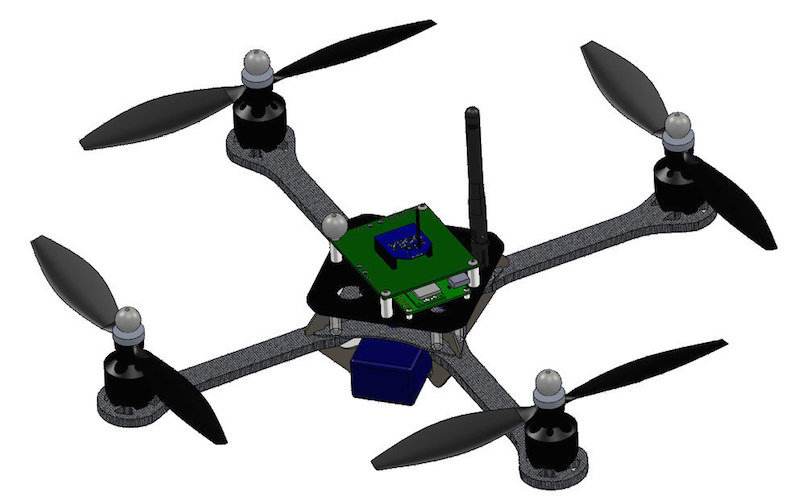
\includegraphics[width = 0.6 \textwidth]{img/quadrotor.jpg}
    \caption[Image of Quadrotor.]{Image of Quadrotor \cite{zainquad}.}
    \label{fig:quadrotor}
\end{figure}
Control systems are the foundation of devices which process inputs and produce a corresponding output. Open-loop control refers to control action, which is independent of the output, whereas closed-loop control refers to control action dependent on the output. Within the context of autonomous drone control, a closed-loop control system is essential in order to ensure the drone reacts to its external environment appropriately. The inputs of controllers for drones come from its sensors, such as gyroscopes, accelerometers, LIDAR, infrared and proximity sensors. The controllers for drones use the data from these sensors as inputs to the control system and output a corresponding signal to its motors, which in turn ensure the drone corrects its movement to changes in the external environment. The thrust, as well as rotation of the drone is responsible for its movement. The rotation is altered in three ways: pitch, roll and yaw. 

Pitch relates to the drone’s movement about its lateral axis, meaning a change in pitch will move the nose of the drone up or down. The pitch is controlled by changing the speed of the propellers at the front and back of the drone. Roll relates to the drone’s movement about its longitudinal axis, meaning a change in roll will tilt the drone. Roll is controlled by changing the speed of the propellers on the sides of the drone. Finally, yaw relates the drone’s movement around its vertical axis, which implies a change in yaw will turn the drone left or right. Yaw is controlled by changing the speeds of diagonal rotors.

There are many different types of control systems used in autonomous applications, with the state-of-the-art controller being a Proportional-Integral-Derivative (PID) controller. Research on new and improved control systems has been conducted over the past decade, with new controllers utilising Model Predictive Control (MPC) and learning-based control (such as neural networks) showing better performance in applications such as medical surgery, imagery and navigation \cite{zain11,zain9}. This improvement in performance is due to two reasons. Firstly, a PID controller requires mathematically modelling the drone’s dynamics and therefore can be computationally intensive for complex environments. Additionally, when mathematically modelling the drone’s dynamics, assumptions such as linearisation must be made which reduces the accuracy of the controller. In learning-based approaches where non-linearities can be accounted for, such as Artificial Neural Networks (ANN), the computational power required as well as accuracy can be improved. 

This project aims to implement a novel approach, using an Adaptive Neuro-Fuzzy Inference System (ANFIS) controller. This approach combines the benefits of using a neural network, with the benefits of fuzzy logic. Fuzzy logic allows for values in a universe to have an uncertain degree of membership and can therefore enable complex systems to be modelled in a less computationally demanding way. This approach has showed promising results within the context of other applications such as electrical conductivity prediction and control of medical devices \cite{boxi1,zain11}. Research within utilising ANFIS in the controllers of autonomous underwater vehicles has also provided a basis for further investigation in other applications. 

New commercially available software has applications and functions which allow ANFIS to be built in a more comprehensive and tailored way. In MathWorks release of MATLAB 2023a, they introduced a Fuzzy Logic Designer App which provides tools to design and tune complex fuzzy inference systems. The findings in literature, coupled with the advancements in software capabilities in this field, allow us to investigate using ANFIS in drone control.
 
\section{Research Problem}
The three issues associated with drones currently are: the cost, accuracy and reliability. Current commercial drones may solve one of these issues, or maybe two if considering accuracy and reliability. However, they have not yet effectively solved all three of these issues. Drone control is the key problem. PID controllers have drawbacks outlined in the project background which cause drone controllers to be computationally intensive. Therefore, this makes them larger and more expensive. Additionally, assumptions such as linearisation result in room for improvement in their control response. A learning based approach which is computationally efficient may allow all three parameters of success to be met. 
\section{Aims and Objectives}
The overall goal of this project is to design and implement an ANFIS (Adaptive Neuro-Fuzzy Inference System) to drone control and evaluate its effectiveness against PID control. The objectives and constraints are the following:

\begin{itemize}
  \item Build a simulation environment either from scratch or using existing simulators, in which parameters such as checkpoints and obstacles can be defined. The simulator should also allow for randomised simulation environments to increase the diversity of the datasets generated.
  \item Gather a dataset of greater than 500,000 datapoints (specified by our industry partners, MassiveAnalytic) with a wide range of simulation scenarios included, such that the drone training data encompasses simplified real world scenarios. 
  \item Perform data pre-processing methods using standard feature selection techniques. A training, validation and test dataset should be produced in order to adequately build and evaluate the ANFIS. 
  \item Build the ANFIS structure, using validation data to tune membership functions in order to minimise training and validation error. Justified ANFIS design decisions will be made to minimise testing error. 
  \item Implement the ANFIS into the simulator and test the ANFIS controller against the PID controller. The two performance metrics of error in position and computational power (number of Bytes of memory required) as well as computational time will be compared and evaluated.
  \end{itemize}

The main constraints relate to the limitations in software when designing the simulator and the ANFIS and computational power of the machine used to perform the data collection from the simulator. 
\begin{itemize}
  \item The more popular and commercially used simulation environments for drones such as Gazebo and ROS are difficult to integrate with the best software for building an ANFIS controller such as MATLAB and Python.
  \item Software that builds neuro-fuzzy inference systems is still being refined and improved. Hence, the resources available to design fuzzy inference systems and refine parameters such as the membership functions are limited. A key example of this is the inability to ``tune'' fuzzy inference systems with more than one output. For this project the Fuzzy Logic Designer Application released in MATLAB 2023a will be used however the 2024 version is likely to have improvements which we will be unable to incorporate.  
  \item As this is a fourth year project, there is a limited time frame (nine months) in which results have to be produced and refined therefore the depth of the analysis is limited. This constraint is particularly relevant to the optimal configuration and implementation of the controller as well as the size of the dataset used to train the ANFIS.
  \item Computational limitations when using personal laptops will be a constraint on the length and magnitude of the simulations and ANFIS built.  
  \end{itemize}
\section{Report Structure}
This report consists of six chapters where research, design and test the implementation of the ANFIS controller in a drone application is explored. 

\textbf{Chapter 1} - Presents the problems background as well as the aims and objectives of the project.

\textbf{Chapter 2} - A comprehensive literature review of the applications and success of neuro-fuzzy systems as well as the control methods currently used for drone dynamics. 

\textbf{Chapter 3} - Provides a detailed overview of the simulation environment created and reasoning for the assumptions and parameters chosen. 

\textbf{Chapter 4} - Explains the process and considerations when building and implementing the ANFIS system into the simulation environment. 

\textbf{Chapter 5} - Summarises and discusses the results of the various ANFIS configurations and the comparison between using the ANFIS controller versus the PID controller in the drone simulation. 

\textbf{Chapter 6} - Reflects on the findings and suggests possible future work.

Figure \ref{fig:generalFlow} shows the design methodology used in this project. 
\begin{figure}[H]
    \centering
    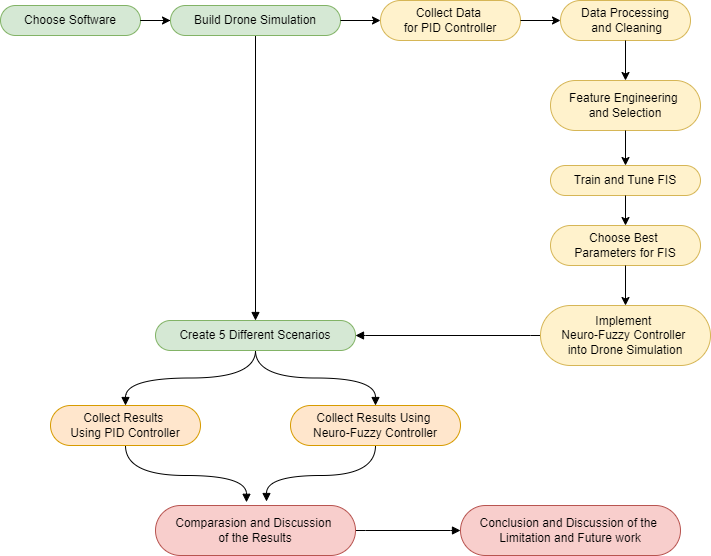
\includegraphics[width = 0.8 \textwidth]{img/generalflow.drawio.png}
    \caption{Flow Diagram of Methodology}
    \label{fig:generalFlow}
\end{figure}
\chapter{Literature Review}
\section{Drone Dynamics and Control}
\subsection{Drone Dynamics}
Mathematical models form the basis of any description of a dynamic system. There are large bodies of literature dedicated to modelling a quadrotors dynamics, to various complexities. The dynamic model seeks to describe the 3D position of the quadrotor. In aircraft terms, this is usually described with measurements such as altitude, and longitude / latitude coordinates. This may also be accompanied with a heading - the direction the aircraft is facing relative to a compass. Other measurements exist to define the position and direction of a drone within a 3D space. The dynamic model is a set of mathematical equations comprising of the sum of forces acting on the system at a time $t$. The various models can be divided into two main categories: models that do not incorporate the motor (body models) and models that do incorporate the motor (propulsion system modelling). The latter type may also incorporate the propellers into the model \cite{hd1}.

DiCesare \textit{et al} present a Lagrangian model for a quadrotor, utilising the `thrust of each motor' as a control input \cite{hd2}. Waslander \textit{et al} utilise a Newton-Euler method to derive a body model, also giving an approximate relationship between motor torque and voltage applied to the motors \cite{hd3}. Acakpovi \textit{et al} use a quaternion representation to achieve body modelling, seeking to achieve a more comprehensive and adaptable body model \cite{hd4}. Das \textit{et al} address the complexities and unknowns of certain elements of the mathematical model by using a backstepping approach and neural nets on their Lagrangian body model to estimate aerodynamic forces and moments \cite{hd5}. All of these models utilise various assumptions such as, the body is rigid and centre of mass and structure are coincident and symmetrical. From these works, the fact that there are numerous approaches to body models, where different goals and capabilities can be seen. The different models underline the importance of both the physical components and the mathematical relationships in understanding and controlling drone behaviour for particular applications.

Propulsion system models can present themselves in various levels of complexity. The vast majority of physical drones and consequently, drone models within literature, use brushless DC motors.  Wierema presents the modelling case of a brushless DC motor in the context of drones \cite{hd6}. Bouabdallah \textit{et al} derive a linearised DC motor model to be used in conjunction with a Lagrangian body model \cite{hd7}. Köroğlu presents a neural network approach to model the motor \cite{hd8}. Propeller modelling also falls under the scope of increasing the granularity and accuracy of the drone model. %Huang \textit{et al} identify the various aerodynamic coefficients and equations of a propeller blade in the context of a drone \cite{hd-drone-modeling} CHECK. 
Ryll \textit{et al} combine a Newton-Euler body model with a propeller model to achieve full controllability over the degrees of freedom of a quadrotor \cite{hd9}. Pounds \textit{et al} robustly model propeller flapping within their mathematical model to achieve a more accurate model \cite{hd10}. Motor models and the integration of propeller models, as showcased in the literature, underscore the increasing sophistication and precision required in advancing drone control, with increasingly granular models seeking to solve specific issues. 
\subsection{Drone Control}
The field of automated control for flying vehicles has been the subject of significant scientific interest. Control techniques rely on simplifying models, with limited states and inputs. However, it is essential to consider what are the critical elements for these reduced models to ensure the reliability of the control guidelines when applied to real aircraft. The quadrotor is a highly sophisticated flying vehicle owing to its exceptional versatility and manoeuvrability, enabling it to carry out a diverse range of tasks \cite{li6}. 

Robust control systems have gained considerable attention in mitigating parameter uncertainties and external disturbances. Uncertainties arising from changes in propeller rotation, blade flapping, propeller rotation speed, and the position of the centre of mass require the use of a robust nonlinear controller, especially in the case of quadrotors. Maintaining control over all six degrees of freedom in quadrotors is challenging due to the limited number of control inputs relative to the number of degrees of freedom; in essence, quadrotors represent an under-actuated system \cite{EMRAN2018165}. To regulate the height, speed, and direction of drones, the altitude controller plays a crucial role in guiding the drone during take-off and landing phases, while control of the drone's direction and speed is vital for successful flight over designated way-points. Li \textit{et al} propose a propose an altitude controller that consists of a PD control term and an acceleration feedback term for a tail-sitter UAV \cite{li7}. 

To meet these control requirements, a variety of control systems can be employed, such as proportional-integral derivative (PID), linear quadratic regulator (LQR), sliding mode control (SMC), fuzzy logic, neural network (NN), and others \cite{li8}. PID controllers are commonly used in autopilot systems due to their simple implementation, but they have limitations in unexpected and hostile environments. Linear quadratic regulation (LQR) provides optimal control methods for managing dynamic systems by minimising an appropriate cost function. When LQR is combined with a linear quadratic estimator (LQE) and a Kalman filter, the result is known as a Linear Quadratic Gaussian (LQG) controller \cite{li9}. Sliding mode control is a nonlinear control technique that employs a discontinuous control signal to direct the system to ``slide'' along a predetermined trajectory. On the other hand, Model Predictive Control (MPC) is another nonlinear approach used to govern UAVs. MPC employs a dynamic model of the system to forecast future states and solve optimal control problems online while minimising error. 

Analysing the literature researched above, traditional methods such as PID, LQR, and sliding mode control offer certain advantages, they may exhibit limitations when faced with unpredictable or hostile environments. Thus, the exploration of more adaptive, nonlinear approaches such as MPC, fuzzy logic, and neural networks in literature seems promising, potentially leading to more effective control in terms of adaptability, error minimisation, and trajectory optimisation.
\begin{comment}
There are several challenges and limitations in controlling the pitch, yaw, and roll dynamics of quadrotor drones. These include: 

Nonlinear and Coupled Dynamics: The dynamic equations of motion for quadrotor drones are inherently nonlinear and coupled, making it difficult to design efficient and robust controllers \cite{Rehan17}. This nonlinearity stems from factors such as aerodynamic effects, motor and propeller dynamics, and the interaction between rotational and translational motions. Traditional linear control techniques may not provide adequate performance and stability in scenarios requiring stabilisation due to multi-angle disturbances, requiring the development of advanced nonlinear control strategies \cite{7016810,hd-cite3}.

External Disturbances: Drones are susceptible to disturbances such as wind, which can significantly impact their stability and control performance. Controllers must be capable of adapting to these disturbances to maintain the desired flight trajectory. Moreover, disturbances can vary rapidly in magnitude and direction, demanding robust and adaptive control algorithms that can adjust in real-time to maintain stability and performance \cite{Kangunde2021}.

Actuator Limitations: The motors and propellers used in quadrotor drones have limitations in terms of their maximum and minimum thrust levels, as well as their response times. These limitations can affect the drone's ability to achieve the desired pitch, yaw, and roll angles. Additionally, actuator saturation or failure can lead to a loss of control authority, making it challenging to maintain stability and perform desired manoeuvres \cite{Joshi2022}. 

Sensor Noise: The onboard sensors, such as inertial measurement units (IMUs) and GPS, are susceptible to noise and inaccuracies, which can impact the controller's ability to estimate the drone's state. These uncertainties can propagate through the control loop and degrade the overall performance and stability \cite{190940}. Advanced filtering techniques, such as the Extended Kalman Filter or the Particle Filter, are often employed to mitigate the effects of sensor noise and improve state estimation \cite{hd-kalman_filter}. 

Model Uncertainty: Accurate mathematical models of quadrotor dynamics are essential for control design. However, these models may not perfectly capture the real-world behaviour of the drone due to factors such as unmodelled aerodynamic effects, manufacturing imperfections, and changes in mass distribution due to payload or battery depletion \cite{hd-drone-modeling}. Model uncertainty can lead to a mismatch between the controller's assumptions and the actual drone dynamics, resulting in reduced performance and potential instability \cite{hd-uav_modelling}.  

Computational Constraints: Advanced control algorithms often require significant computational resources to solve complex optimization problems or implement adaptive techniques in real-time. The limited processing power and memory available on small drones can constrain the choice of control algorithms and their implementation, potentially impacting the overall control performance. Drones | Free Full-Text | Computationally-Efficient Distributed Algorithms of Navigation of Teams of Autonomous UAVs for 3D Coverage and Flocking (mdpi.com) Miniaturizing the brain of a drone | Robotics @ MIT 

Robustness and Fault Tolerance: Ensuring robustness and fault tolerance in quadrotor control systems is crucial for maintaining stability and preventing catastrophic failures in the event of component malfunction, such as motor or sensor failure Fault-Tolerant Control of an Hexarotor Unmanned Aerial Vehicle Applying Outdoor Tests and Experiments - ScienceDirect. Designing controllers that can automatically detect and adapt to such failures, or even enable the drone to perform a controlled emergency landing, remains a significant challenge Automated Emergency Landing System for Drones: SafeEYE Project | IEEE Conference Publication | IEEE Xplore viewcontent.cgi (usu.edu). 
\end{comment}
\subsection{Model Predictive Control}
Model Predictive Control (MPC) is a increasingly popular control method tested in several applications including autonomous vehicles and medical uses. The results from literature for MPC suggest that it is a robust and efficient control method, however can be inflexible and hard to implement in some cases. As there has been more extensive testing on MPC, this review looks to find literature that compares the use of ANFIS and MPC controllers. 

A research paper by Rodriguez \textit{et al} tested designs for a controller for exoskeletons, devices used augment patient rehabilitation, specifically in a re-configurable exoskeleton for lower limbs \cite{zain11}. In this paper, the performance of PD, ANFIS and MPC controllers were tested in this application and can be seen in Figure \ref{fig:mpc}. This shows that the MPC and ANFIS controllers have a lower average error in position than the PD controller. When comparing the MPC and ANFIS controller results, the MPC is better at certain points, however, the paper concludes that the ANFIS controller performs better for this application. This shows the flexibility and ease of implementation of ANFIS could result in it being favourable in complex applications.  
\begin{figure}[H]
    \centering
    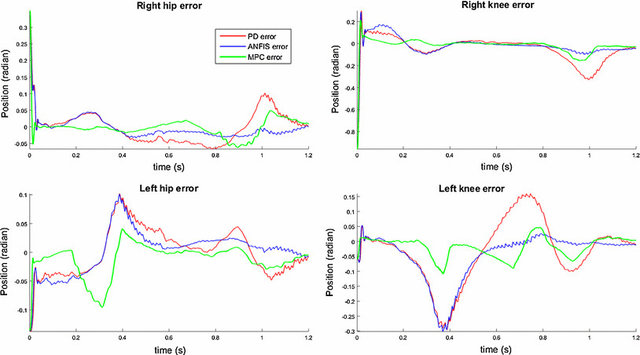
\includegraphics[width = 0.75\textwidth]{img/mpc_results.jpg}
    \caption[Research paper showing error in positions results for PD, ANFIS and MPC controllers]{Research paper showing error in positions results for PD, ANFIS and MPC controllers \cite{zain11}.} 
    \label{fig:mpc}
\end{figure} 
\subsection{Extended Kalman Filter}
The Kalman Filter is an efficient optimal estimator that provides an iterative computational methodology for estimating the state of a discrete-data controlled process from measurements that are usually noisy, whilst also giving an estimate of the uncertainty of the estimates \cite{zain12}. The Extended Kalman Filter (EKF) is an extension of this, where non-linearities are accounted for. This method can also be used as an alternative to the PID control method and has proven to be useful in literature. 

Few papers have been written directly comparing the use of EKF and learning-based methods for controllers as most papers compare the results of PID, MPC and learning-based approaches. This could suggest that EKFs are known to be less effective for controllers and therefore investigating this in recent years has not been worthwhile. A journal by Aydogmus \textit{et al} compared the use of Extended Kalman Filter and ANN approaches to estimate shaft speed for a closed-loop control system \cite{zain14}. This paper found that the Artificial Neural-Networks (ANN) implementation produced better performance than the EKF. Another research paper by Cuevas \textit{et al} directly compared an ANFIS model to an EKF model in the application of gaze control \cite{zain13}. Gaze control refers to using computational tricks to alter one's gaze. The results from the paper can be seen in Figure \ref{fig:kalman}. The results show that the EKF has a much higher number of frames at a higher error. These studies support the fact that EKF methods may generally be regarded as inferior in control applications when compared to learning-based approaches. 
\begin{figure}[H]
    \centering
    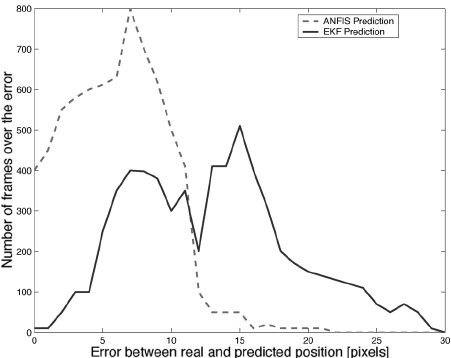
\includegraphics[width = 0.7\textwidth]{img/kalman filter.png}
    \caption[Performance results of EKF compared with ANFIS for gaze control]{Performance results of EKF compared with ANFIS for gaze control \cite{zain13}.}
    \label{fig:kalman}
\end{figure} 
\subsection{Neural Network Based Control}
Learning-based controllers use different variations of neural network approaches. As the framework of neural networks is inspired by the human brain and is a widely used machine learning method,  it follows that variations of this learning-based technique are used for controllers. 

A research paper by Arora \textit{et al} compared the use of ANN and ANFIS based controllers for grid connected photovoltaic (PV) systems. As PV arrays have non-linear characteristics, from changing temperature and solar irradiation, these learning-based algorithms are crucial for tracking maximum power from the PV array \cite{zain9}. The control response for both controllers were compared and the ANFIS controller had a lower settling time, overshoot, and fewer oscillations when compared with the ANN controller. Conclusively, in this application, an ANFIS controller performed better. 

Another research paper by Uluocak \textit{et al} analysed the use of different learning models applied to an Eddy Current Dynamometer \cite{zain10}. An Eddy Current Dynamometer is an instrument used to convert mechanical energy to electrical energy. This paper found that the ANFIS model performed better than the Radial Basis Neural Network (RBNN) and the Single Hidden Layer Neural Network (SHLNN) as it produced the lowest Mean Absolute Percentage Error (MAPE). As a result, it can be concluded from literature, that in complex control applications, ANFIS is likely to provide the most promising results. 
\section{Current Studies on Neuro-Fuzzy Controllers}
\subsection{Review on fuzzy-neural network controllers} 
Adaptive Neuro-Fuzzy Inference System (ANFIS) is a powerful hybrid method, which combines the advantages of fuzzy logic and neural networks to establish an efficient decision-making system \cite{boxi1}. Recently, ANFIS has significant applications in unmanned aerial vehicles (UAVs) such as path planning and obstacle avoidance. In this review, we will study the existing literature on ANFIS-based control systems compared with conventional proportional integral derivative (PID) controllers for the operation of UAVs and autonomous drones. 
%When ANFIS is used in the optimisation of the autonomous drones, the collected data from using a traditional PID controller act as inputs ($x$ and $y$) in Figure \ref{fig:anfis}. 

Figure \ref{fig:anfis} shows a generic ANFIS architecture, accepting inputs from a PID controller. In this instance $x$ and $y$ represent two generic inputs from data collected from a PID controller. In the fuzzification process seen in Layer 1, the computer reacts like a human brain and gives out linguistic outputs, such as ``low speed''. Layer 2, the product layer, then determines the rules that will be used to make decisions based on the fuzzy variables generated in Layer 1. At this stage, an optional normalisation layer can be implemented, however, if the inputs are already between 0 and 1, this can be excluded. Layer 4, the defuzzification layer, then converts the outputs from Layer 2 / 3 into a defuzzified output that feeds into the output layer \cite{boxi2}. 
\begin{figure}[H]
    \centering
    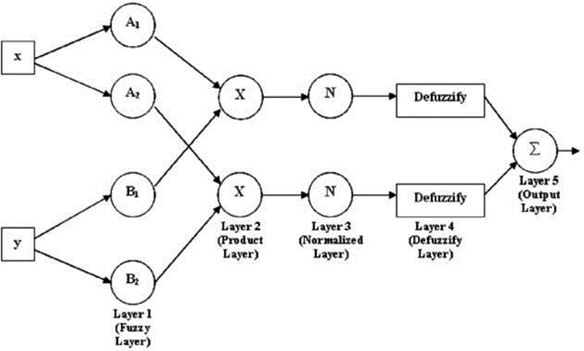
\includegraphics[width = 0.8 \textwidth]{img/Picture1.png}
    \caption[Architecture of an ANFIS model.]{Architecture of an ANFIS model \cite{boxi2}.}
    \label{fig:anfis}
\end{figure}
Recent studies on utilising ANFIS in control applications include an innovative approach for the autonomous flight control of UAVs using ANFIS. ANFIS mainly consists of three stages: input-output mapping, fuzzy inference, and rule optimisation, which can also be implemented into the quadrotors \cite{boxi4}. The input-output mapping stage involves collecting data on the flight performance (altitude, air speed and bank angle), which is then used to train the ANFIS model. The fuzzy inference stage uses the trained ANFIS model to make decisions on the  flight control based on its current and desired states. The rule optimisation stage aims to improve the performance of the ANFIS model by refining the fuzzy rules and adjusting the membership functions. Kurnaz \textit{et al} introduce three fuzzy logic modules to control the three-dimensional position of a UAV by adjusting the roll and pitch angles and throttle position \cite{boxi3}. This ANFIS model has 5 layers, with a hybrid learning algorithm based on a Sugeno inference system, which reduced the response time and made the controller more efficient. 

The authors tested their approach on a simulated UAV and evaluated its performance based on several metrics, including error in altitude, speed, and heading angle. The results in the paper show that the ANFIS-based approach outperforms a conventional PID controller in terms of design simplicity and trajectory following. However, unstable performance is caused by inconsistent ANFIS learning algorithms during the change of environmental conditions such as wind speed. The obstacle avoidance also has similar issues due to the change of positions of obstacles and the learning algorithm should be carefully monitored. This provides a framework and a set of results which can be built on. 

Another approach on quadrotors by Al-Fetyani \textit{et al} presents a novel ANFIS-based control system that integrates a fuzzy inference system (FIS) and a neural network (NN) to enhance the accuracy and robustness of the drone control system, particularly its attitude (direction relative to the horizon line) and altitude performances \cite{boxi5}. The article outlines the design and implementation of ANFIS, which involves three stages: data collection, model training, and controller development. Attitude and altitude data is collected from a flight simulation using a classical PD controller. The ANFIS-PD controller is trained and designed by a neuro-fuzzy designer. The training stage gives the membership functions for the inputs of altitude and attitude errors as well as their error rates. 

The design methodology involves building an ANFIS-based model to predict the output values of the drone's attitude and altitude control systems. The data acquisition and pre-processing steps involve collecting sensor data from the drone and filtering it to remove noise and outliers, which makes the data clearer and easier to process by ANFIS. Therefore, data cleaning after collection is a necessary step to ensure the ANFIS model can be trained optimally. The performance of controllers is evaluated using simulation experiments, where the quadrotor is subjected to various flight scenarios. 

Case 1 is taken from Luukkonen’s research on modelling and control of quadrotor \cite{boxi6}. The simulation results shown in Figure \ref{fig:referencepic} demonstrate that the ANFIS-PD controller can achieve the desired state in the shortest time with minimal overshooting. In addition, the power consumption of PD controller is more than twice as much as the ANFIS controller. As compared with a conventional PD controller, Fuzzy-PD still has a better performance.
\begin{figure}[H]
    \centering
    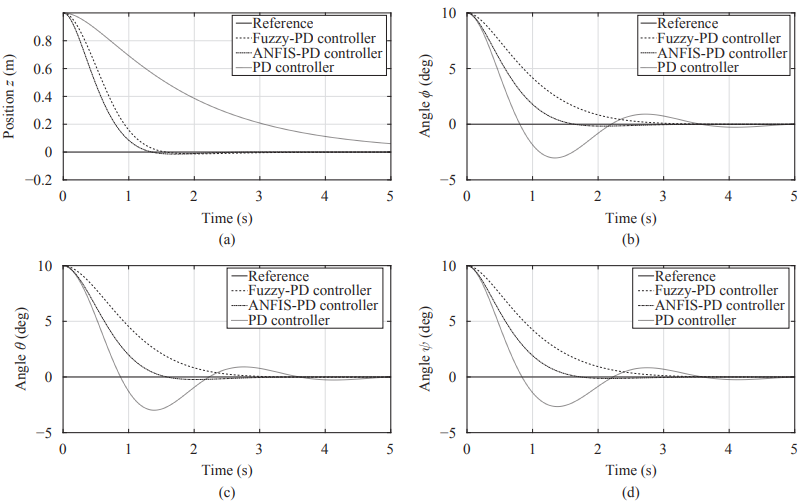
\includegraphics[width = 0.7 \textwidth]{img/Picture2.png}
    \caption[Simulation results for case 1: (a) Position z; (b) Angle $\phi$; (c) Angle $\theta$; (d) Angle $\varphi$.]{Simulation results for case 1: (a) Position z; (b) Angle $\phi$; (c) Angle $\theta$; (d) Angle $\varphi$ \cite{boxi5}.}
    \label{fig:referencepic}
\end{figure}
This analysis was then built on by Al-Fetyani to develop a case 2. In this case, the desired state varies over time. Since the PD controller is tuned to a near hovering state, within the time interval of 10-\SI{15}{\second}, oscillations occur while attempting to regulate the angular positions $\phi$ and $\varphi$. In comparison with PD and Fuzzy-PD controllers, the time required for ANFIS-PD controller to reach the desired state is still the fastest in this case. A case 3 was then developed, which looked into the performance of the controllers in following a desired altitude when subjected to disturbances. In this case of the ANFIS-PD controller, it has considerable resilience in the presence of external forces. The analysis performed on these cases also provide a basis for further analysis and once again shows the potential improvements applying ANFIS in a controller provides. 

The results show that the ANFIS can improve the attitude and altitude performances of the drone, which has low error rates with external disturbance force and fastest response times to reach a time varying state compared to conventional control methods. In the quadrotor, results of positions in $x$, $y$ and $z$ direction for different cases using fuzzy neural controller and PID controller are compared with the desired position. Another approach is on trajectory tracking of marine rescue drone by Pham and Han \cite{boxi7}. The main challenge in these operations is the ability to accurately track a desired trajectory and compensate for disturbances such as wind. The neural network estimates the drone's position and velocity based on sensor data, and the fuzzy logic controller generates control signals based on the estimated position and velocity. Simulations of PID and fuzzy neural controllers adjusting $z$ position of the drone are carried out in the conditions of presence and absence of wind. The graph of attitude varies with time from Figure \ref{fig:picture5} and Figure \ref{fig:picture6} demonstrates that the fuzzy neural controller is much more effective than a PID controller. 
\begin{figure}[H]
\centering
\begin{minipage}{.5\textwidth}
    \centering
    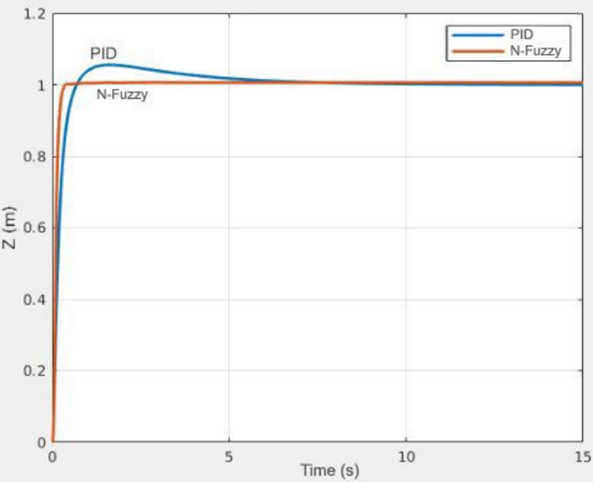
\includegraphics[width=0.95\linewidth]{img/Picture5.png}
    \caption[Simulation result of attitude against time for PID and N-Fuzzy controllers without wind.]{Simulation result of attitude against time for PID and N-Fuzzy controllers without wind \cite{boxi7}.}
    \label{fig:picture5}
\end{minipage}%
\begin{minipage}{.5\textwidth}
    \centering
    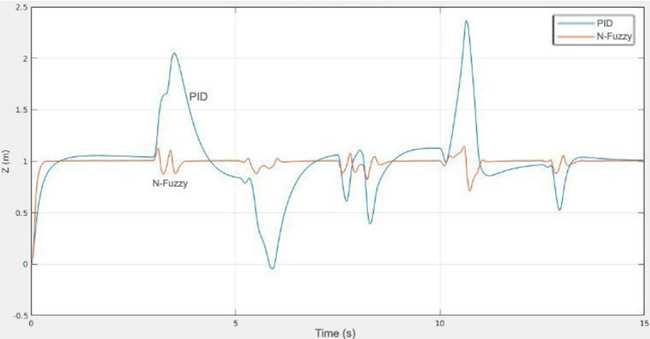
\includegraphics[width=0.95\linewidth]{img/Picture6.png}
    \caption[Simulation result of attitude against time for PID and N-Fuzzy controllers with wind.]{Simulation result of attitude against time for PID and N-Fuzzy controllers with wind \cite{boxi7}.}
    \label{fig:picture6}
\end{minipage}
\end{figure}
The graph of drone’s thrust over time using PID and neural fuzzy controller in Figure \ref{fig:picture7} and Figure \ref{fig:picture8} illustrates that the neural fuzzy controller has a shorter response time than the PID controller, with a more effective reaction on the action of wind. In the case of the drone's obstacle avoidance, the simulation result is also comparable to the performance of the two controllers with and without disturbance.

The performance of ANFIS was evaluated using simulations and experiments, and the results showed that the neuro-fuzzy controller was able to accurately track the desired trajectory and compensate for disturbances. It reaches a stable state faster with a larger thrust, which improves the efficiency by 67\% and reduced the response time by 85\% compared with PID controllers \cite{boxi7}. This study demonstrates the performance metrics used to evaluate both controllers and shows the use of error in $z$ position and error in thrust as the two chosen response curves.   
\begin{figure}[H]
\centering
\begin{minipage}{.5\textwidth}
    \centering
    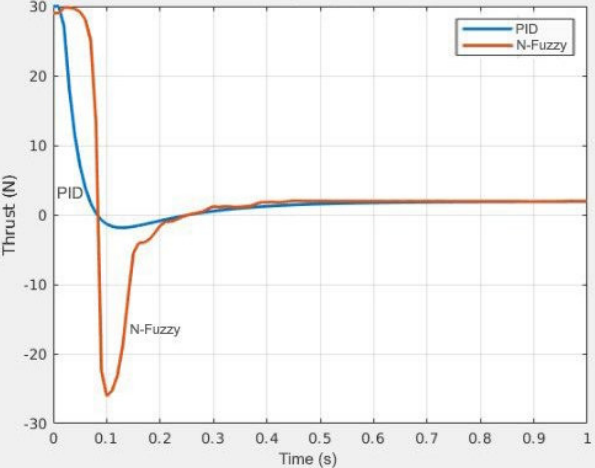
\includegraphics[width=0.95\linewidth]{img/Picture7.png}
    \caption[Simulation result of thrust against time for PID and N-Fuzzy controllers without wind.]{Simulation result of thrust against time for PID and N-Fuzzy controllers without wind \cite{boxi7}.}
    \label{fig:picture7}
\end{minipage}%
\begin{minipage}{.5\textwidth}
    \centering
    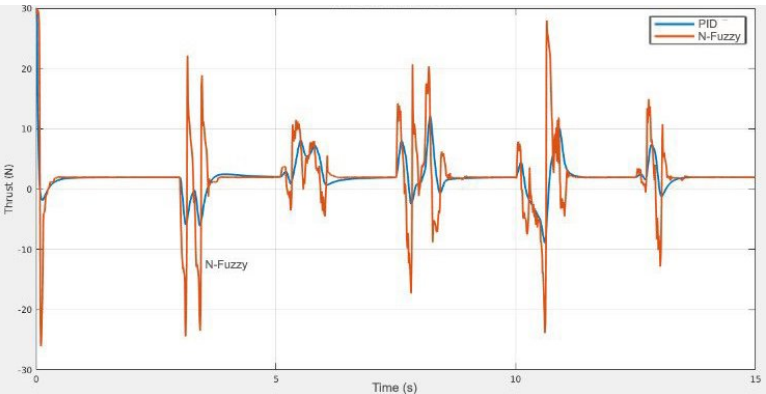
\includegraphics[width=0.95\linewidth]{img/Picture8.png}
    \caption[Simulation result of thrust against time for PID and N-Fuzzy controllers with wind.]{Simulation result of thrust against time for PID and N-Fuzzy controllers with wind \cite{boxi7}.}
    \label{fig:picture8}
\end{minipage}
\end{figure}
\subsection{Type-1 and Type-2 Fuzzy Inference Systems} 
Fuzzy Inference Systems (FIS) have been widely used in the development of autonomous drones for various applications. Type-1 and Type-2 FIS are inference systems where two different types of fuzzy sets are used to build the FIS. Type-1 FIS is based on crisp logic and is the most common FIS in autonomous drones \cite{boxi8}. However, more recent studies are analysing the use of Type-2 FIS and whether, in some applications, these types perform better.

Research on Type-2 fuzzy systems by Castañón-Puga \textit{et al} is an extension of Type-1 fuzzy systems that can handle uncertainties and non-linearity in the input data \cite{boxi9}. A self-learning Type-2 fuzzy system is presented, which is a system that can adapt and learn from data in real time. The Type-2 FIS was developed in order to build a mobile application that uses Wi-Fi signals to obtain indoor locations. Therefore, for this application, this study found that a Type-2 fuzzy system was more adequate. 

A case study of a self-learning Type-2 FIS by Al-Mahturi is applied to the control of an autonomous underwater vehicle \cite{boxi10}. The system uses data from the vehicle’s sensors and the result shows that Type-2 FIS can effectively identify the system’s dynamics and control the vehicle’s motion to follow a desired path, concluding that self-learning Type-2 fuzzy systems have great potential in system identification and control of autonomous systems. 

A study by Ontiveros \textit{et al} compared Type-1 and Type-2 systems in medical diagnosis \cite{zain3}. The conclusions of the study were that for data sets with low uncertainty, Type-1 fuzzy inference systems performed the best and that for data sets with medium and high uncertainty, Type-2 FIS performed the best. Therefore, despite the use of Type-2 systems in autonomous underwater vehicles and results from Al-Mahturi \textit{et al}, the best configuration of FIS for a drone application will highly depend on the data set used to train the FIS. 

\subsection{Sugeno versus Mamdani Fuzzy Inference Systems} 
Mamdani and Sugeno are two Fuzzy Inference Systems (FIS) developed by Takagi-Sugeno and Professor Ebrahim Mamdani. Mamdani FIS is characterised by its defuzzification output of membership function, whereas Sugeno FIS has a crisp output computed by a weighted average \cite{boxi11}. As a result, Sugeno FIS are generally better in applications of optimisation, pattern recognition and control systems whereas Mamdani FIS are better in applications of education, training, consumer-orientated applications and highly complex applications. Both have been used in various applications of drone technology, including trajectory tracking, obstacle avoidance, and aerial surveillance.

In trajectory tracking, Mamdani FIS has been used to control the movement of drones. For example, in the study by Pham and Han, a combined neural network and Mamdani FIS was used to control the trajectory of a marine rescue drone \cite{boxi7}. The Mamdani FIS was used to determine the velocity and heading of the drone based on the input variables, which included the current location of the drone, the location of the target, and the obstacle avoidance status. It provides a smooth and stable control of the drone trajectory. 

In aerial surveillance, both Mamdani and Sugeno FISs have been used to analyse the data collected by drones. In a study by Yanar \textit{et al}, a Mamdani FIS was trained on a dataset of images labelled with distinct levels of natural hazards and was able to accurately classify the new images captured by the drone \cite{boxi13}. 

In obstacle avoidance, Sugeno FIS has been used to control the movement of drones in complex environments. In the study by Haidar \textit{et al}, a hybrid control system consisting of Sugeno FIS and PID controller was proposed for drone obstacle avoidance \cite{zain7}. Based on the input variables including the obstacle’s distance and direction, the desired heading of the drone is determined by a Sugeno FIS. The velocity of the drone is adjusted by the PID controller according to the error between the desired and actual heading. The hybrid control system provided a fast and accurate obstacle avoidance for the drone. Therefore, in light of this literature, for a drone control application, the optimisation of obstacle avoidance through ANFIS may be best achieved through the implementation of Sugeno FIS due to its crisp output. 

\subsection{ANFIS Membership Functions} 

Membership functions characterise the degree of ``membership'' of values in a set. These functions are what differentiate fuzzy sets from classical sets. Within classical sets, these memberships would only have discrete values of 0 and 1. Fuzzy sets allow uncertainty in the membership of values in a universe to be factored in. When building an ANFIS model, the choice of membership functions for the inputs will impact the accuracy of the output values. 

A research paper that looked at the prediction of unsaturated hydraulic conductivity using an ANFIS analysed the performance of various membership functions, namely the triangular, generalised bell-shaped and Gaussian functions \cite{656546546}. The results of this study suggested that the use of Gaussian membership functions improved the performance, when compared with triangular and generalised bell-shaped. 

Additionally, as Gaussian membership functions have more recently been identified as the optimal membership functions for fuzzy inference systems, some studies have focused on developing improved Gaussian membership functions. A study by Zhang \textit{et al} looked to derive adaptive Gaussian-shaped membership functions for four separate datasets \cite{zain6}. Despite showing improved performance, these methods were hard to implement in practical applications where the current software is not up to date.

\section{Simulation environments and data collection}
The accuracy and performance of drone simulations is crucial aspect to test the performance of a drone. Simulations test the performance of the drone in a virtual environment and help the researcher to understand the relationship between different onboard parameters \cite{roy1}. For example, the rotor speed and the mass of the drone are key to a drone's design and performance. As a result, the ability to understand how these variables change the drone dynamics when testing the drone in simulations is helpful. Metrics such as stability could be tested before implemented on a real drone, reducing time cost and prototyping cost. Also, different algorithms could affect the performance of a drone and can be tested without risk. This is suitable for specific cases such as a drone operating in an extreme environment. Based on the hardware performance, software simulation also acts as an efficient method for testing, where a researcher could run multiple simulation simultaneously and rapidly. This is a key advantage compared to collecting data in the real-world as running multiple simulations provides several datasets for further investigation and developing for the drone design. 

Simulations are software based and are traditionally built on mainstream platforms such as Windows and Linux. Different softwares have different functionality and goals. Hence, it is important to choose an environment which provides the fidelity and accuracy required in our specific application. Table \ref{tab:simulators} shows a comparison of some drone simulators and their respective functionalities \cite{Roy5}. 

\begin{table}[H]
    \centering
    \footnotesize
    \setlength\tabcolsep{2pt}
    \begin{tabular}{@{}lllllll@{}}
        \toprule
        \textbf{Simulator} & \textbf{FlightGear} & \textbf{X-Plane} & \textbf{JMavSim} & \textbf{Gazebo} & \textbf{AirSim} & \textbf{UE4Sim}\\
        \midrule
        Commercial/free & Free & Commercial & Free & Free & Free & Free \\
        Vehicles & Multirotors & Multirotors & Multirotors & Multirotors & Multirotors & Multirotors \\ 
        & UAVs & UAVs & & Robots & & Cars \\
        & Airplanes & Airplanes & & & & \\
        Interface ROS   & No   & No         & Yes  & Yes  & No   & No \\
        Sensors         & Diversity of & Easy incorporation & No incorporation & Easy modification & Monocular, & Easy modification  \\
        & sensors & of sensors & of sensors & of sensors & depth cameras, & of sensors \\
        &  &  &  &  & no lidar &   \\
        Motion capture      & No     & No     & No   & No   & Yes    & Yes    \\
        Obstacles           & Yes    & Yes    & No   & Yes  & Yes    & Yes    \\
        SITL-HITL           & Yes    & Yes    & Yes  & Yes  & Yes    & No     \\
        MAVLink             & Yes    & Yes    & Yes  & Yes  & Yes    & No     \\
        Ease of Development & Medium & Medium & High & High & Medium & Medium \\
        \bottomrule
    \end{tabular}
    \caption[Comparison of Available UAVs Simulators.]{Comparison of Available UAVs Simulators \cite{Roy5}.}
    \label{tab:simulators}
\end{table}

AirSim is a new simulation platform which is based on the Unreal Engine and released in 2017 \cite{roy2}. It is an open source software, and it supports deep learning, computer vision and reinforcement learning algorithms for UAV and vehicles. From the previous research based on this software, AirSim includes a physics engine that can operate at high frequencies for real-time hardware-in-the-loop (HITL) simulations \cite{roy3}. HITL simulation testing is executed in real time and it is integrated with the physical hardware. In general, it is used when components of the simulation tasks are complex for instance a high number of power converters, plants or feedback sensors. \cite{ELLIS2012261}. It is supported by popular protocols such as MavLink \cite{roy3}. Although AirSim provides high-fidelity results, it does not support code generation, resulting in less flexibility. Also, the high-fidelity results make using AirSim time-consuming and computationally intensive. Consequently, it is not suitable for large dataset generation. 

MATLAB is another option for simulation process of drone dynamics. One of the key benefits is that Simulink allows a wide range of sensors to be applied \cite{roy1}. An example of using the ANFIS framework in MATLAB is seen within a study looking at the deployment of photovoltaic systems where the current-voltage is nonlinear \cite{roy6}. Power is generated from a solar panel and after data collection, the aim is to calculate the maximum power. The research aims to use the ANFIS which is based on MATLAB / Simulink to investigate the maximum power or maximum utilisation of the photovoltaic system. The implementation of this system is between the solar panels and the power regulation devices. In this paper, all the results, except the circuit design, are based on MATLAB and Simulink. The result is a new control system from ANFIS training, which is high-efficiency, enabling the user to trace the maximum utilisation path in the context of several weather conditions. This shows the use of MATLAB and Simulink working effectively in literature and therefore it can be deemed to be a suitable software for developing control systems.
\chapter{Simulation Design}
\section{Choice of Software}
The simulation environment was created using MATLAB and Simulink. MATLAB provides a comprehensive environment, with support for packages such as the UAV Toolbox, for simulating UAVs. MATLAB also has support for Path Planning and Navigation Toolboxes for generating flight trajectories and an Autopilot and Control Systems Toolbox for designing and analysing a controller. Another key advantage to MATLAB and Simulink is the integration and support for ANFIS controllers. This will allow development of our ANFIS controller in the same environment as our simulator, easing development. 

The simulator was heavily adapted from an existing example on UAV Obstacle Avoidance from Simulink. By modifying and adding our own elements to the Simulink programme, a bespoke solution for data collection was achieved. Autonomous scenarios and drone control allowed for data collection without the need for manual input, saving a large amount of time, and allowed for concurrent simulations to run, increasing the amount of data collected.
\section{Simulink Structure}
The developed Simulink model is shown in Figure \ref{fig:sim1} and is based on a model from MathWorks. Many different ``blocks'' can be seen, divided into three main sections:
\begin{itemize}
    \item UAV Scenario
    \begin{itemize}
        \item UAV Scenarios Motion Read: captures current UAV state
        \item UAV Scenario LIDAR: captures LIDAR sensor data
        \item UAV Scenario Scope: visualisation of trajectory and LIDAR data
        \item UAV Scenario Configuration: configuration of scenario
        \item UAV Scenario Motion Write: updates UAV state
    \end{itemize}
    \item Waypoint following and obstacle avoidance
    \begin{itemize}
        \item Waypoint Follower: computes a lookahead point for the UAV
        \item Obstacle Avoidance: 3D VFH+ algorithm is used to calculate a safe direction and yaw for unobstructed flight, updating the Waypoint Follower block's lookahead point accordingly
        \item Enable Obstacle Avoidance: enable or disable obstacle avoidance
    \end{itemize}
    \item Controller and plant
    \begin{itemize}
        \item Controller: responsible for generating control signals for the UAV
        \item Quadrotor Plant: updates UAV state with control signal
    \end{itemize}
\end{itemize}
These concepts are explained in detail in later sections.
\begin{figure}[H]
    \centering
    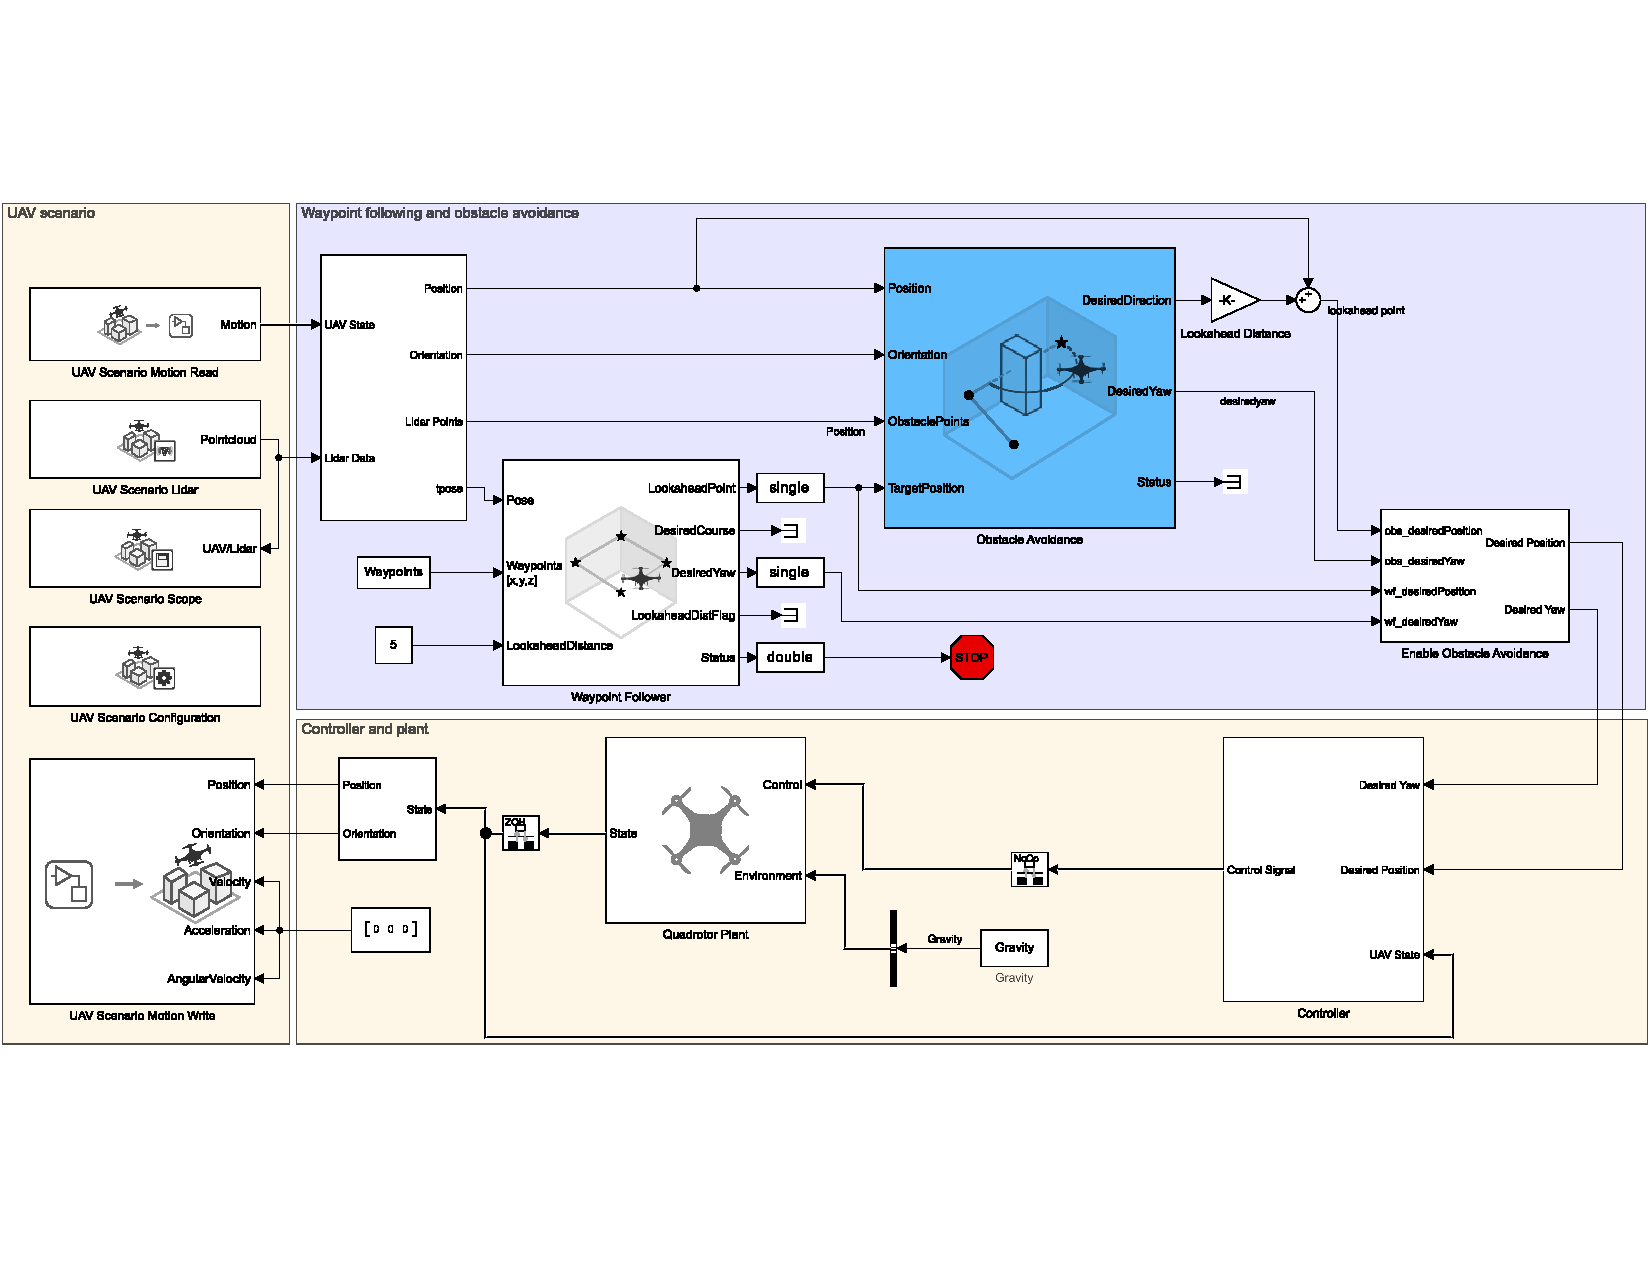
\includegraphics[width =\textwidth]{img/simulink_model.pdf}
    \caption{Simulink model.}
    \label{fig:sim1}
\end{figure}
A key addition for the data collection was the addition of random scenario generation to the model. Further, for the data collection, some of the parameters and function of the blocks in the diagram above were re-coded. The significant change to the simulation is the waypoints and obstacles generation. In the original Simulink process and code, the waypoints and the obstacles were fixed. Hence, a new function code was required in order to replace the fixed waypoints generator. Random waypoint generation is crucial to allow for a range of scenarios and motions to be recorded during simulation. This is to capture as much of the drone dynamics as possible, in order to train the fuzzy inference system with a wide and robust set of data.
\subsection{Quadrotor Model}
The quadrotor model used in this project is a generic commercial quadrotor. A commercial quadrotor such as a DJI drone is highly versatile and has all the specifications available. Also, using a commercial model means that the results of the simulation are representative of real-world use. Additionally, the cost of the quadrotor is likely to be lower than educational products. A complete set of sensors is also installed. Therefore, the commercial quadrotor is the best option in this case.

The quadrotor used in the simulation has mass \SI{1}{kg} and radius \SI{10}{cm}. These values are representative of a generic small-to-medium-sized quadrotor. The quadrotor model in the simulator uses a reduced-order guidance block. This block uses a closed-loop system, which includes the UAV dynamics and autopilot. It is used for small multi-rotor UAVs. Although this may not be the most realistic nor accurate model, as it is reduced order, it provided results which can be easily used and extracted. The autopilot gains are kept the same as in the original model. The following equations govern the quadrotor model. The position of the UAV in the world frame is:
\begin{equation}
    \begin{bmatrix} x & y & z\end{bmatrix}
\end{equation}
The orientation, roll, pitch, and yaw, is: 
\begin{equation}
    \begin{bmatrix} \phi & \theta & \psi\end{bmatrix}
\end{equation}
The respective angular velocities are: 
\begin{equation}
    \begin{bmatrix} p & q & r\end{bmatrix}
\end{equation}
The model takes a commanded roll, pitch, yaw rate, and total thrust:
\begin{equation}
    \begin{bmatrix} \phi^{Control} & \theta^{Control} & \dot{\psi}^{Control} & F^{Control}_{thrust}\end{bmatrix}
\end{equation}
The outputs are the position, velocities, orientation, angular velocities, and thrust:
\begin{equation}
\setcounter{MaxMatrixCols}{20}
    \begin{bmatrix} x & y & z & \dot{x} & \dot{y} & \dot{z} & \phi & \theta & \psi & p & q & r & F_{thrust} \end{bmatrix}
\end{equation}
The rotation matrix $R$ is given by:
\begin{equation}\label{rotation matrix}
R=
\begin{bmatrix}
\cos{\theta}\cos{\psi} & \cos{\psi}\sin{\phi}\sin{\theta}-\cos{\phi}\sin{\psi} & \cos{\psi}\cos{\phi}\sin{\theta}+\sin{\phi}\sin{\psi}\\
\cos{\theta}\sin{\psi} & \cos{\phi}\cos{\psi}+\sin{\phi}\sin{\psi}\sin{\theta} & -\sin{\phi}\cos{\psi}+\cos{\phi}\sin{\psi}\sin{\theta}\\
-\sin{\theta} & \cos{\theta}\sin{\phi} & \cos{\theta}\cos{\phi}
\end{bmatrix}
\end{equation}
The acceleration of the drone is given by:
\begin{equation}\label{drone accel}
m
\begin{bmatrix}
\ddot{x}\\
\ddot{y}\\
\ddot{z}
\end{bmatrix}
=
\begin{bmatrix}
0\\
0\\
mg
\end{bmatrix}
+ R
\begin{bmatrix}
0\\
0\\
-F_{thrust}
\end{bmatrix}
\end{equation}
where $m$ is the mass of the drone and $g$ is the acceleration due to gravity. The angular velocities are given by:
\begin{equation}\label{angular velocity}
\begin{bmatrix}
\dot{\phi}\\
\dot{\theta}\\
\dot{\psi}
\end{bmatrix}
=
\begin{bmatrix}
1 & \sin{\phi}\tan{\theta} & \cos{\phi}\tan{\theta}\\
0 & \cos{\phi} & -\sin{\phi}\\
0 & \dfrac{\sin{\phi}}{\cos{\theta}} & \dfrac{\cos{\phi}}{\cos{\theta}}
\end{bmatrix}
\begin{bmatrix}
p\\
q\\
r
\end{bmatrix}
\end{equation}
The block approximates a closed-loop controller for the roll, pitch, yaw rate, and thrust. Roll and pitch are controlled using a PD controller, while yaw rate and thrust are controlled using a P controller. The angular accelerations are given by:
\begin{equation}\label{angular accel}
\begin{bmatrix}
\dot{p}\\
\dot{q}\\
\dot{r}
\end{bmatrix}
=
\begin{bmatrix}
1 & 0 & -\sin{\theta}\\
0 & \cos{\phi} & \sin{\phi}\cos{\theta}\\
0 & -\sin{\phi} & \cos{\phi}\cos{\theta}
\end{bmatrix}
\begin{bmatrix}
KP_\phi(\phi^{Control}-\phi)+KD_\phi(-\dot{\phi})\\
KP_\theta(\theta^{Control}-\theta)+KD_\theta(-\dot{\theta})\\
KP_\psi(\dot{\psi}^{Control}-\dot{\psi})
\end{bmatrix}
\end{equation}
where $KP$ and $KD$ are the proportional and derivative gains. The thrust rate is given by:
\begin{equation}\label{thrust eqn}
\dot{F}_{thrust}=KP_F(F^{Control}_{thrust}-F_{thrust})
\end{equation}
\subsection{Sensors}
The LIDAR sensor sends rapid laser pulses, which are reflected off objects, and receives the response to map out an area. This allows for path planning and obstacle avoidance algorithms to work as it provides a map of the environment in its vicinity. LIDAR creates a point cloud based on the points that the laser reflects back to the sensing unit. This provides information on the distances of each point of the obstacle, mapping the drone’s surroundings.

An alternative for LIDAR is using cameras for photogrammetry systems. Although cameras are cheap, LIDAR has the advantage of being able to works at any time of the day, while cameras may not be able to provide sufficient detail in the dark. Additionally, cameras require high processing capabilities \cite{9278591}.  

Table \ref{tab:zain3} shows the LIDAR sensing unit’s parameters, set to standard ranges given by MathWorks. 
\begin{table}[H]
    \centering
    \begin{tabular}{@{}ll@{}}
        \toprule
        \textbf{Parameter} & \textbf{Value(s)}\\
        \midrule
        Maximum range & \SI{7}{\meter}\\
        Range accuracy & \SI{0.02}{\meter}\\
        Azimuthal limits & \SI{-179}{\degree} to \SI{179}{\degree}\\
        Elevation limits & \SI{-15}{\degree} to \SI{15}{\degree}\\
        Azimuthal resolution & \SI{0.5}{\degree}\\
        Elevation resolution & \SI{2}{\degree}\\
        Sample time & \SI{0.01}{\second}\\
        \bottomrule
    \end{tabular}
    \caption{LIDAR parameters.}
    \label{tab:zain3}
\end{table}
\subsection{Waypoint Following}
The Waypoint Follower block, shown in Figure \ref{fig:wp_follower}, is used to follow a set of waypoints using a lookahead distance, which determines the distance at which the target point - lookahead point - will be. It calculates the lookahead point, desired trajectory, and desired yaw. Its inputs are the current state (position and orientation), the waypoints, and the lookahead distance. Using this information, it calculates an intermediate point for the UAV to move towards, in order to reach the waypoints. The desired position and desired yaw data is crucial to building the neuro-fuzzy controller as these datapoints directly relate to the control signal applied to the drone.
\begin{itemize}
    \item \textbf{Position and Orientation:} The current position and orientation (roll, pitch, yaw) of the UAV.
    \item \textbf{Waypoints:} The coordinates of the waypoints.
    \item \textbf{Lookahead Point:} This is the desired point for the UAV to move to, in order to get closer to the next waypoint. In the setting of this parameter, a minimum and maximum distance are required, which are set as \SI{0.2}{\meter} and \SI{5}{\meter} respectively. The distance determines how far away the lookahead point will be. This output is fed to the Obstacle Avoidance Block.
\end{itemize} 
\begin{figure}[H]
    \centering
    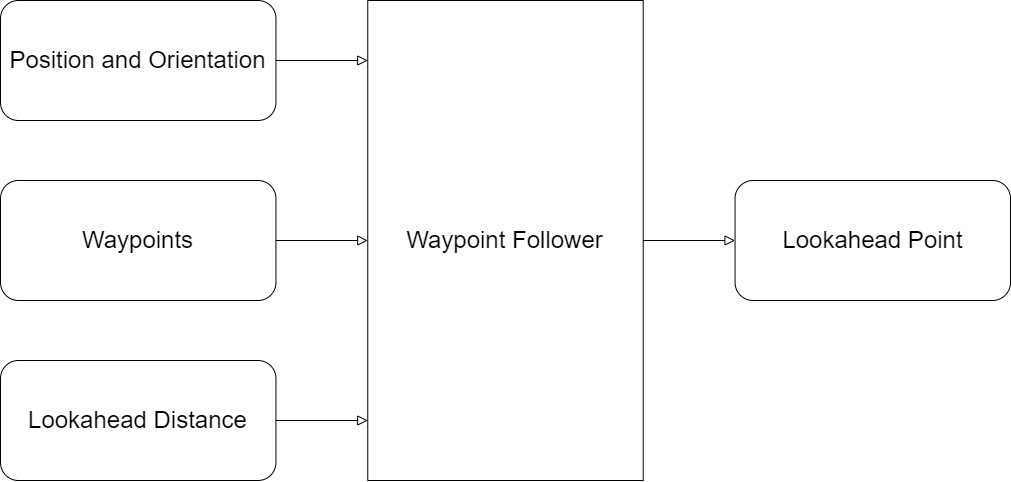
\includegraphics[width = 0.7\textwidth]{./img/wp_follower.png}
    \caption{Inputs and outputs of the Waypoint Follower block.}
    \label{fig:wp_follower}
\end{figure}
When following a set of waypoints, in this case, the drone will most likely ignore the first waypoint as the drone pose is set to start in hover or to start from the ground. The pose of a drone is a combination of its yaw, pitch and roll angle that the drone is actually performed \cite{Roy5}. The initial yaw, pitch and roll angle are zero. Depending on the drone's heading, the drone will try to start from the current waypoint to the next one in a linear path although in a realistic scenario, the drone has to constantly change its heading to stabilise. The pitch, yaw or roll angle is changed, which depends on the difference of altitude and heading between two defined waypoints. In this simulation, paths between each waypoints, including the initial path, are being split into different path segments. In most cases, the drone is driven by the control signal in order to track the path segments. In the second condition, a transition region is introduced in order to smooth the path taken. Based on the nature of the lookahead distance for path tracking, if the quadrotor is within \SI{0.1}{\meter} to the next waypoint, the transition region is used. In the third condition, the lookahead distance is not in the transition region but the drone's heading is about to change. In this case, a 3D hyperplane is drawn at the next waypoint. 

From documentation from Mathworks, a hyperplane is the vector space that is contained in the current space. If the current space is a $n$ dimensional space or vector, the hyperplane of this space or vector will be a $n-1$ dimensional space or vector. For example, on a 2D surface, the hyperplane is a line on the surface. Equivalently, in a 3D space, the hyperplane is a surface inside of this volume. Figure \ref{fig:hyperplane} shows the transition region of the waypoint and the hyperplane region in top view. Once the drone is inside of the hyperplane, the waypoints follower directs the quadrotor from the current waypoint to the next waypoint. One of the boundaries of the hyperplane is perpendicular to the direct path from last waypoint and the next waypoint and it is parallel to the ground surface. This smooths the trajectory to the next waypoint and allows for a more stable flight path. The hyperplane condition is defined by the following equations,
\begin{gather}
    \left(p - w_1 \right)^T\left(w_2 - w_1\right) \geq 0
\end{gather}
where $p$ is the position of the quadrotor, $w_1$ and $w_2$ are sequential waypoint positions. The vector $p$, $w_1$ and $w_2$ has three components, ($x$, $y$, $z$). $T$ represents the transpose of the matrix. $p_1$ is the first scenario that the drone is not in the hyperplane. The red line $p_1$ represents the lookahead distance that is set before the simulation starts. Once the lookahead distance enters into the transition region, the drone starts to turn onto the next path segment. Another scenario is $p_2$, where the drone is in the hyperplane region. In this case, the drone is changing its heading and moving onto the next path segment. The first part of the inequality ($p-w_1$) represents the vector of the displacement between the position of drone $p$ and the position of waypoint $w_1$. The second part of the inequality ($w_2-w_1$) is the vector of the displacement between the waypoint just passed and the next waypoint the drone is heading to. The result of their product is a number. When it less then zero, the specific hyperplane is not used. If the result is equal or larger to zero, the drone determines that it is located inside the hyperplane region. Therefore, the hyperplane condition is enabled.
\begin{figure}[H]
    \centering
    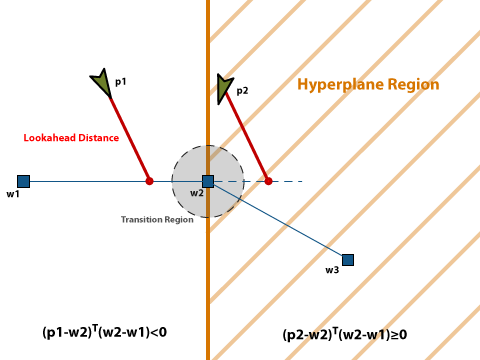
\includegraphics[width = 0.7\textwidth]{./img/fig9.png}
    \caption[Hyperplane illustration.]{Hyperplane illustration from MathWorks.}
    \label{fig:hyperplane}
\end{figure}
\subsection{Obstacle Avoidance}
The obstacle avoidance block from the UAV toolbox is used, a simplified diagram is shown in Figure \ref{fig:obs_avoid}. Obstacle avoidance is enabled through the use of a LIDAR sensor, which allows the algorithm to compute an obstacle-free direction towards a lookahead point, which is determined by the waypoints.
\begin{itemize}
    \item \textbf{Position and Orientation:} The current position and orientation (roll, pitch, yaw) of the UAV.
    \item \textbf{Obstacle Points:} These are obtained from the point cloud from the LIDAR sensor, indicating the points where an obstacle is detected.
    \item \textbf{Target Position:} This is the lookahead point from the Waypoint Follower Block.
    \item \textbf{Obstacle-Free Direction:} The desired direction of movement which does not have an obstacle.
    \item \textbf{Obstacle-Free Point:} The desired point of movement in the obstacle-free direction.
    \item \textbf{Desired Yaw:} The desired yaw in order to turn to the obstacle-free direction.
\end{itemize}
\begin{figure}[H]
    \centering
    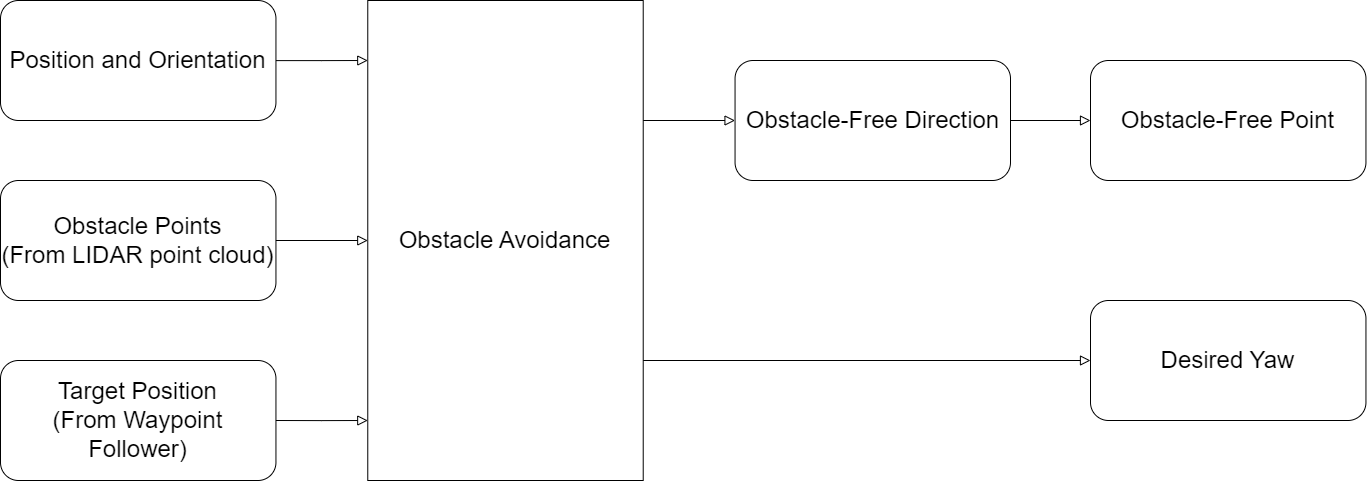
\includegraphics[width = 0.8\textwidth]{./img/obs_avoid.png}
    \caption{Simplified Obstacle Avoidance block.}
    \label{fig:obs_avoid}
\end{figure}
The inputs are the UAV state (position and orientation), the obstacle points, which are given by the LIDAR, and the target position, given by the Waypoint Follower Block as the lookahead point. This block computes a desired direction and yaw for the drone to move. This is then fed into the lookahead distance, which finds the furthest point in the desired direction where there is no obstacle. These are then fed into the controller.

A cost function is used determine the desired direction. This is defined using the target direction, current direction, previous direction, and their associated weights. The weights for these are 5, 2, 2 respectively. The highest weight is in the target direction, meaning deviating from the target direction will be penalised more heavily than the other directions. The block finds the minimum of the cost function to determine the desired direction and yaw for the drone.
\section{Simulation Environment}
The simulation environment is designed using random obstacle and waypoint generation, thereby allowing for a wide range of scenarios to be simulated. The map size is \SI{50}{\meter} $\times$ \SI{50}{\meter}. This is chosen to have a lower computational time, whilst still having a dense environment for the drone to navigate.

Three to four cuboid obstacles are generated with varying dimensions. This is to simulate a high density environment for the drone to navigate. The dimensions for the obstacles are chosen to be less than one-quarter of the map size, and represent various obstacles. For example, buildings are represented as obstacles with lengths and widths of greater than \SI{8}{\meter}, and small trees are represented as obstacles sized around \SI{1}{\meter} to \SI{3}{\meter}. The height is chosen to be up to around five storeys or \SI{20}{\meter}, to account for the varying height of buildings, trees, and other obstacles.

Three to six waypoints are generated randomly, represented as discs that are \SI{5}{\meter} below the actual waypoint position in the environment. This is done to prevent the drone from crashing into the discs, while still allowing for visualisation of the waypoints. This number of waypoints are chosen to allow the drone to navigate a large portion of the environment, thereby requiring more manoeuvres to be completed, for a rich dataset. The properties of the environment are shown in Table \ref{tab:zain5}.
\begin{table}[H]
    \centering
    \begin{tabular}{@{}ll@{}}
        \toprule
        \textbf{Parameter} & \textbf{Value(s)}\\
        \midrule
        Map Size & \SI{50}{\meter} $\times$ \SI{50}{\meter} \\
        Number of Waypoints & 3 to 6\\
        Number of Obstacles & 3 to 4 \\
        Obstacle Width & \SI{1}{\meter} to \SI{13}{\meter}\\
        Obstacle Length & \SI{1}{\meter} to \SI{13}{\meter}\\
        Obstacle Height & \SI{5}{\meter} to \SI{20}{\meter}\\
        \bottomrule
    \end{tabular}
    \caption{Simulation environment parameters.}
    \label{tab:zain5}
\end{table}
 A generated scenario is shown in Figure \ref{fig:sim_pic_5}. Two obstacle maps are created. One to check for any intersections between obstacles and waypoints, and another where the scenario will run. For the map used to check for intersections, the obstacles and waypoints have dimensions increased by \SI{1}{\meter} on each side of the lengths and widths. This ensures that in the real simulation map, there will be a minimum distance of \SI{2}{\meter} between obstacles, allowing the drone to move between obstacles.
\begin{figure}[H]
    \centering
    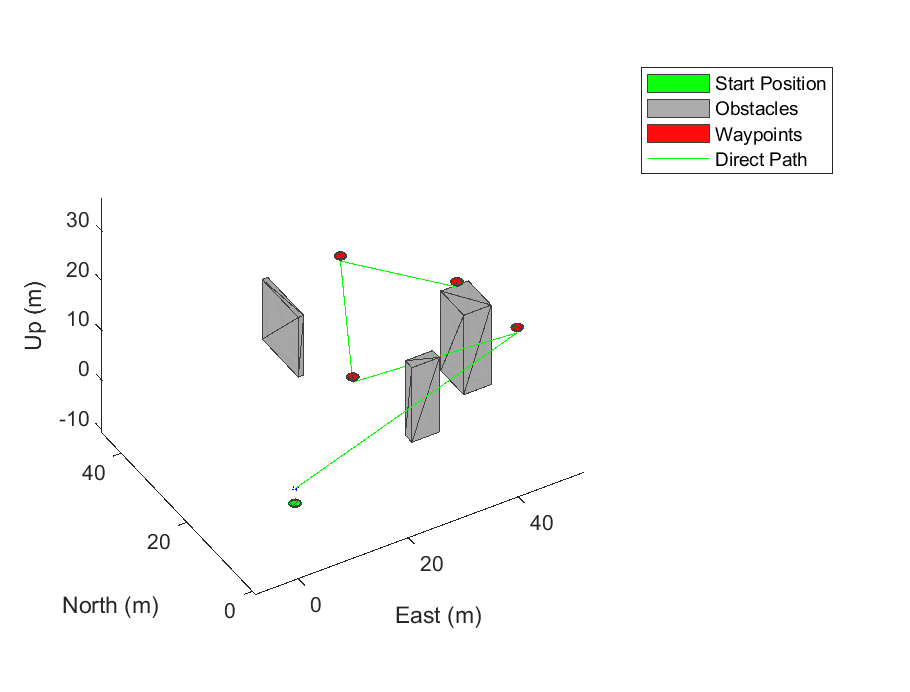
\includegraphics[width = 0.75\textwidth]{./img/sim_pic_5.eps}
    \caption{Randomly generated scenario.}
    \label{fig:sim_pic_5}
\end{figure}
In the simulator, the UAV will navigate to the next waypoint, in order, while moving to avoid any obstacles in its way. In a scenario where the waypoints are of the same height, such as in Figures \ref{fig:sim_pic_1} and \ref{fig:sim_pic_4}, it is able to simulate the flight of the quadrotor without colliding with obstacles. Additionally, the drone does not need to reach the exact location of the waypoint; it only needs to be within \SI{0.1}{\meter}, then it will move on to the next one, as seen in the same figure. The LIDAR sensing can be seen as a point cloud on the surface of an obstacle, seen in Figure \ref{fig:sim_pic_1} and Figure \ref{fig:sim_pic_4}, with the colour of each point indicating the distance away from the drone. This allows visualisation of what the drone can and cannot detect as it navigates through the environment, and enables obstacle avoidance.
\begin{figure}[H]
    \centering
    \begin{minipage}[b]{0.45\textwidth}
        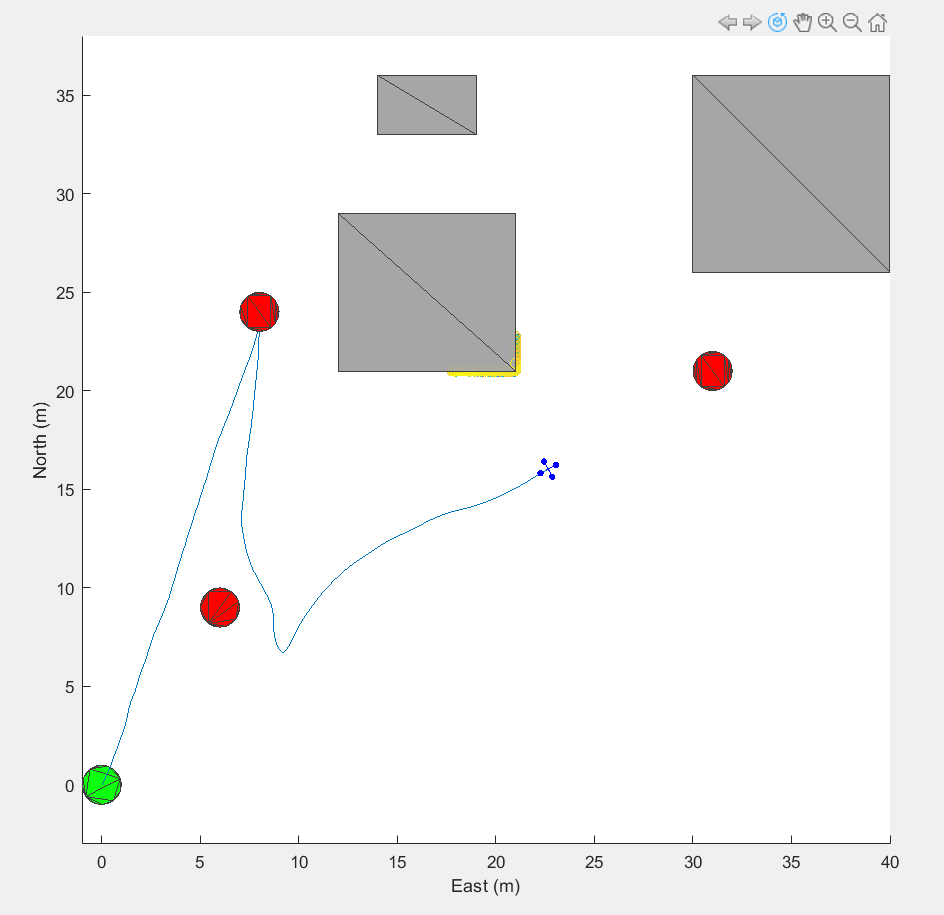
\includegraphics[height=7cm,keepaspectratio]{./img/sim_pic_1.png}
        \caption{Movement of drone in a random scenario with waypoints at the same height.}
        \label{fig:sim_pic_1}
    \end{minipage}
    \hfill
    \begin{minipage}[b]{0.45\textwidth}
        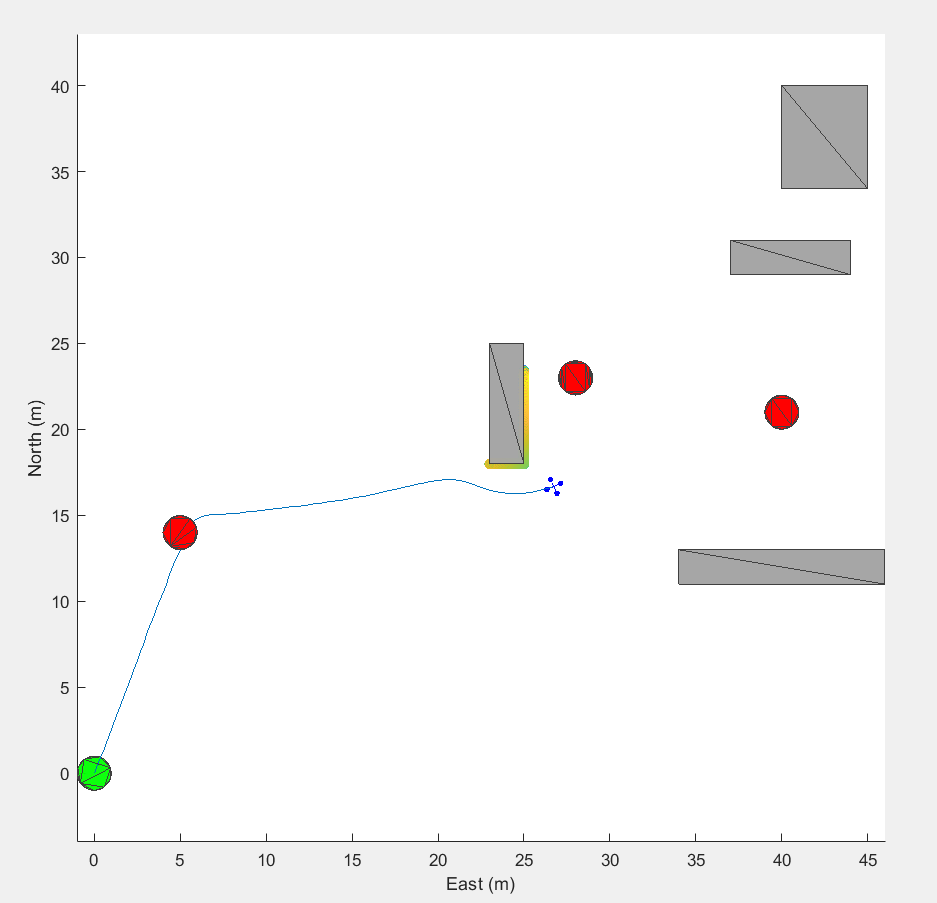
\includegraphics[height=7cm,keepaspectratio]{./img/sim_pic_4.png}
        \caption{Movement of drone in typical scenario. Point cloud on can be seen on obstacle near the drone.}
        \label{fig:sim_pic_4}
    \end{minipage}
\end{figure}
In scenarios where the waypoints differ in height, the behaviour of the drone changes. This is shown in Figure \ref{fig:sim_pic_2}. When ascending or descending, the drone moves in a spiral motion. This may be due to the LIDAR not being able to detect vertically upwards and downwards; therefore the drone attempts to spiral instead of moving vertically. This can be seen in Figure \ref{fig:sim_pic_3}.
\begin{figure}[H]
    \centering
    \begin{minipage}[b]{0.45\textwidth}
        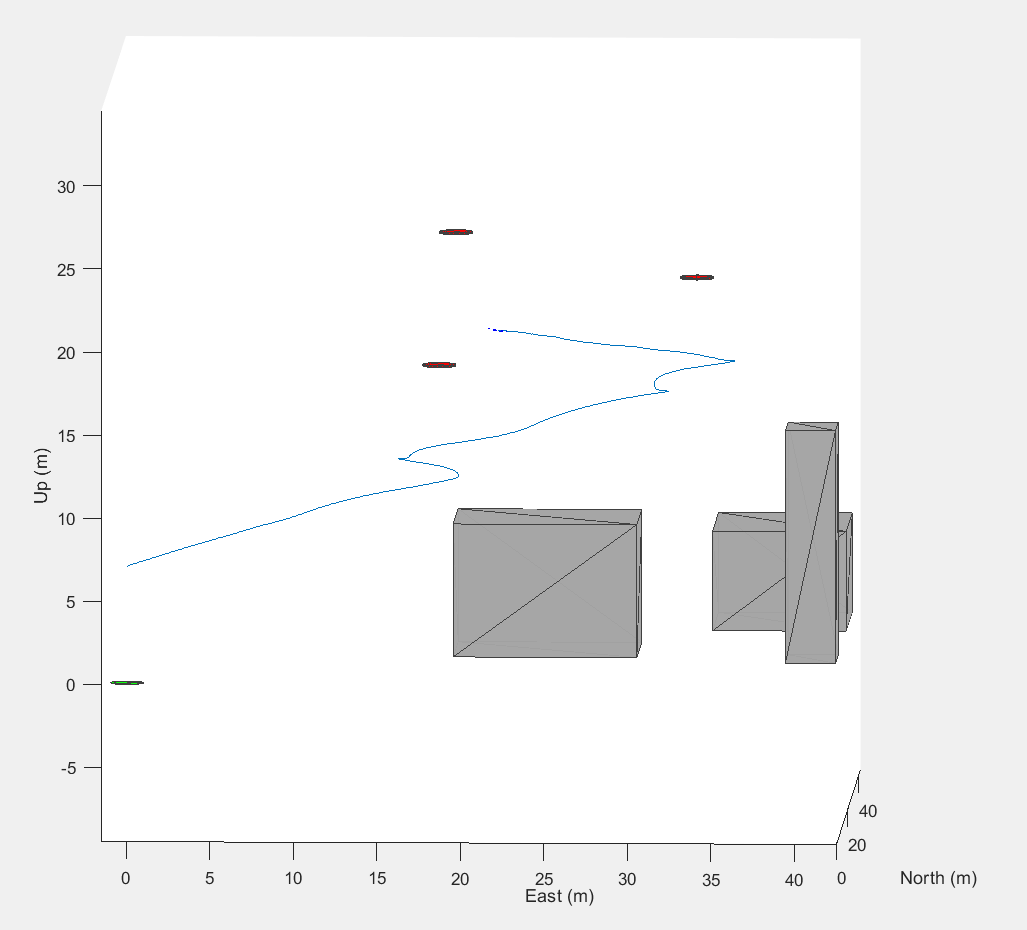
\includegraphics[height=7cm,keepaspectratio]{./img/sim_pic_2.png}
        \caption{Movement of drone in a random scenario with waypoints at the different heights.}
        \label{fig:sim_pic_2}
    \end{minipage}
    \hfill
    \begin{minipage}[b]{0.45\textwidth}
        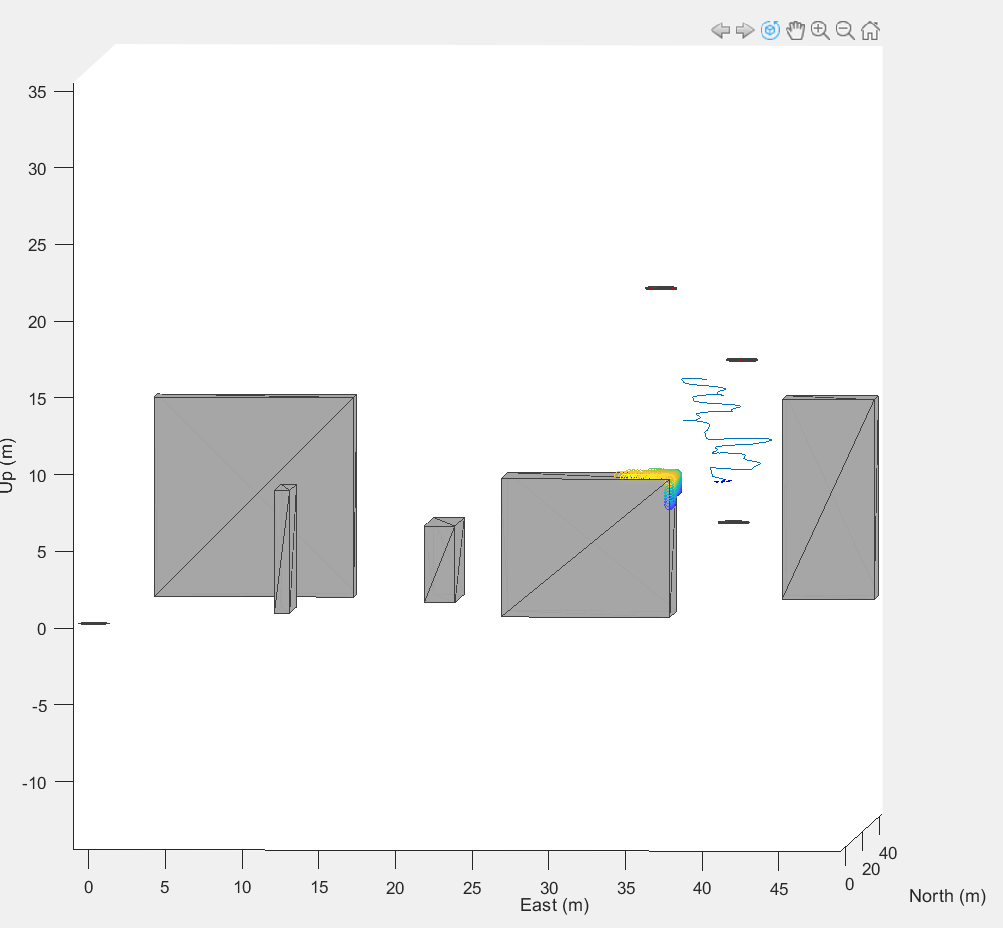
\includegraphics[height=7cm,keepaspectratio]{./img/sim_pic_3.png}
        \caption{Spiralling path of drone as drone descends.}
        \label{fig:sim_pic_3}
    \end{minipage}
\end{figure}

\section{Scenarios}
Five scenarios are created to compare the FIS controller and PID controller. These aim to put the drone in different environments, such as in open air without obstacles, or in urban environments where the drone must navigate through buildings.

\subsection{Scenario 1}
The first scenario is shown in Figure \ref{fig:3_3_scenario1}. It does not have any obstacles, to test the controller in an open air environment. This scenario aims to test the controller in navigating waypoints of different heights with a small turn, without any obstacle avoidance. 
\begin{figure}[H]
    \centering
    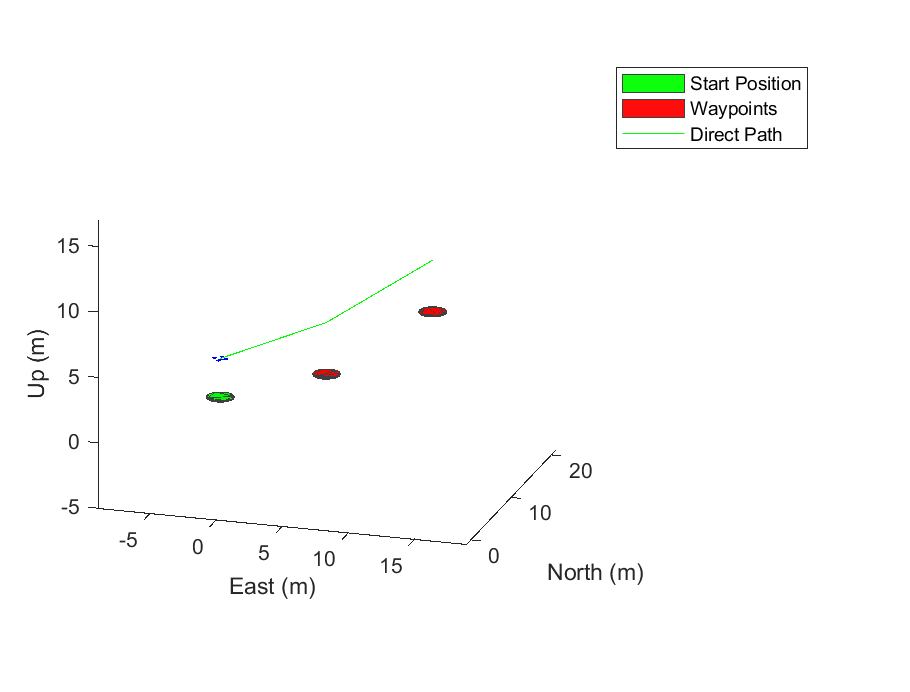
\includegraphics[width = 0.6\textwidth]{./img/3_3_scenario1}
    \caption{Scenario one in open air with no obstacles.}
    \label{fig:3_3_scenario1}
\end{figure}

\subsection{Scenario 2}
The second scenario is shown in Figure \ref{fig:3_3_scenario2}. It consists of two obstacles, with one obstructing the direct path. This scenario aims to test the controller when there is an obstacle involved. It imitates moving between two obstacles, for example two trees. This tests how well the controller can control a change in direction to avoid the obstacle, and the second obstacle serves to prevent excessive turning in this manoeuvre.
\begin{figure}[H]
    \centering
    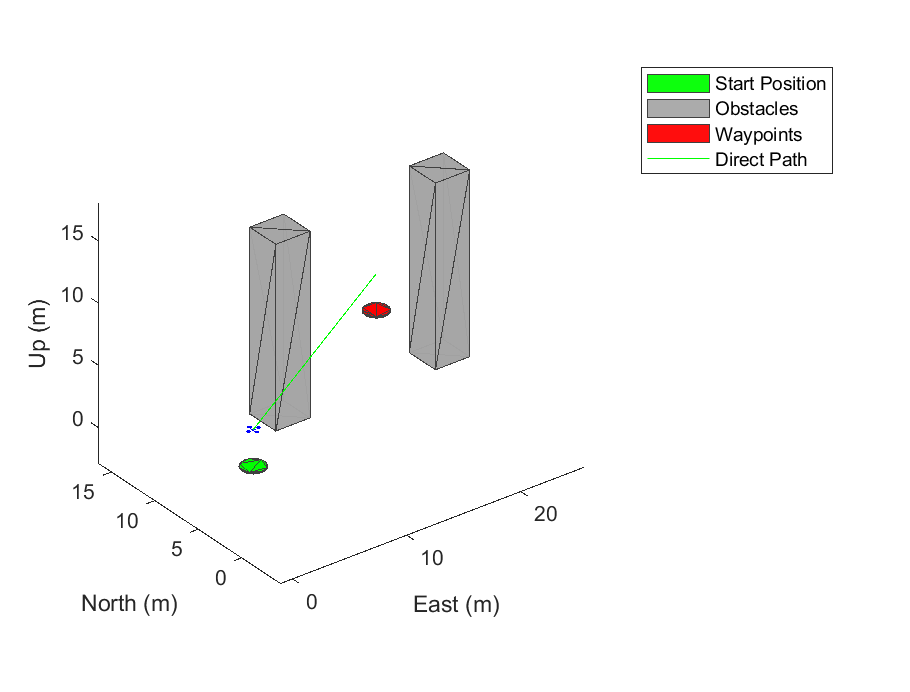
\includegraphics[width = 0.6\textwidth]{./img/3_3_scenario2}
    \caption{Scenario two with a simple obstacle avoidance manoeuvre.}
    \label{fig:3_3_scenario2}
\end{figure}

\subsection{Scenario 3}
The third scenario is shown in Figure \ref{fig:3_3_scenario3}. This scenario is used to test the controller when ascending and descending, to go over an obstacle. This incorporates obstacle avoidance and altitude change to see the movement when the drone senses obstacles beneath it instead of in front of it.
\begin{figure}[H]
    \centering
    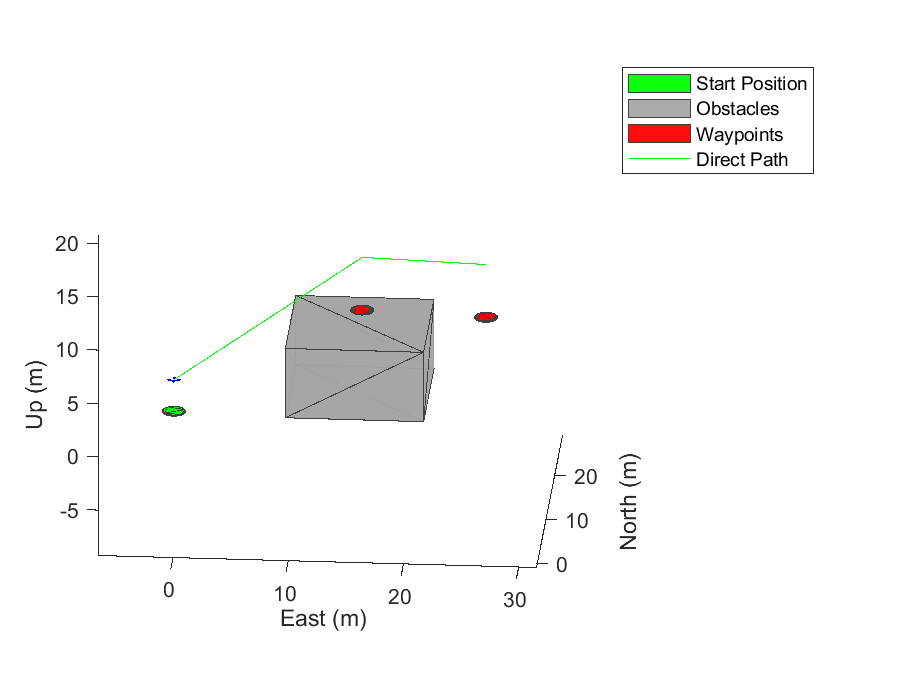
\includegraphics[width = 0.6\textwidth]{./img/3_3_scenario3}
    \caption{Scenario three with a height-varying obstacle avoiding manoeuvre.}
    \label{fig:3_3_scenario3}
\end{figure}

\subsection{Scenario 4}
The fourth scenario is shown in Figure \ref{fig:3_3_scenario4}. This scenario is similar to scenario two, with the addition of an extra waypoint and a change in height of the waypoints. It tests the controller's ability to move around an obstacle, like a pillar or tree. The sharp turn from the first to second waypoint is also another testing point for the controller.
\begin{figure}[H]
    \centering
    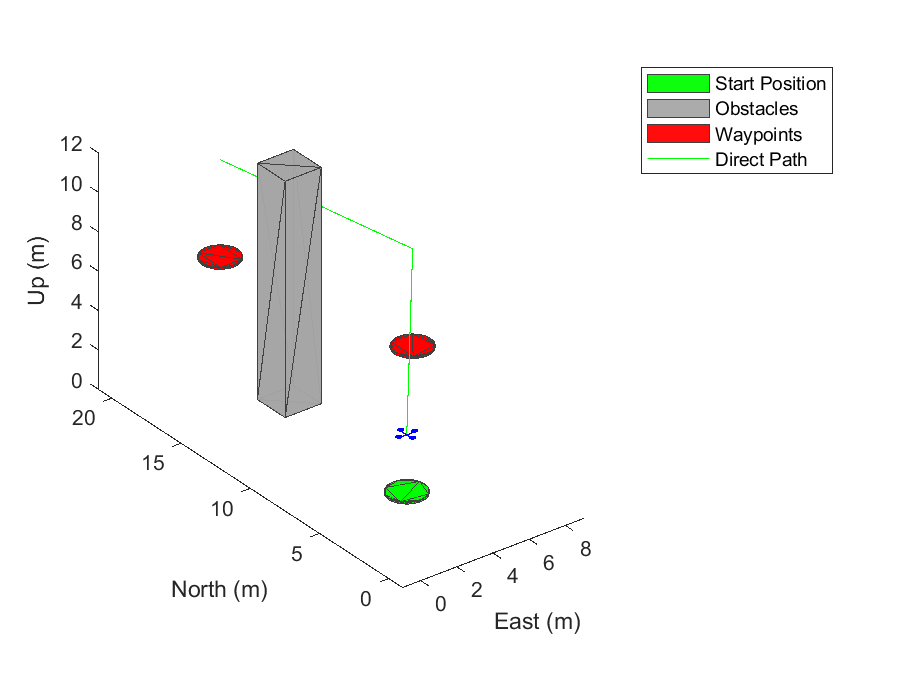
\includegraphics[width = 0.7\textwidth]{./img/3_3_scenario4}
    \caption{Scenario four involves change in height and obstacle avoidance.}
    \label{fig:3_3_scenario4}
\end{figure}

\subsection{Scenario 5}
The fifth scenario is shown in Figure \ref{fig:3_3_scenario5}, the waypoints are all at the same height. This scenario is inspired by urban navigation. It aims to replicate an urban environment, to see the performance of the drone in dense and compact spaces. This is to test movement that involves traversing between obstacles and relatively narrow areas. 
\begin{figure}[H]
    \centering
    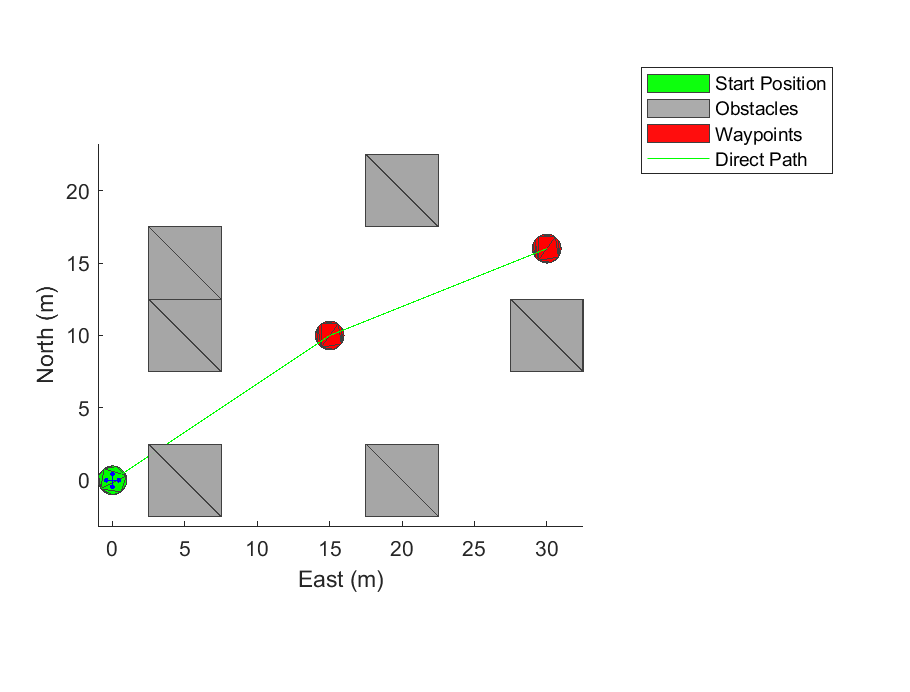
\includegraphics[width = 0.7\textwidth]{./img/3_3_scenario5}
    \caption{Scenario five imitates an urban environment for obstacle avoidance.}
    \label{fig:3_3_scenario5}
\end{figure}
\chapter{Implementation}\label{implementation}
\section{Data Collection and Exploration}
In order to train the neuro-fuzzy controller, data from the simulation using PID controller was collected. To reduce overfitting and to train the controller for all scenarios, the simulations from which data was to be collected had randomised waypoints and obstacles. The data from 40 simulations each with a sample rate of \SI{0.01}{\second} was collected giving a total of 505,075 datapoints, representing \SI{84}{\minute} of drone operation.  
 
There were 18 inputs and 4 outputs collected, shown in Table \ref{tab:inputsOutputs}.
\begin{table}[H]
    \centering
    \begin{tabular}{@{}llll@{}}
        \toprule
        \textbf{Inputs}& & \textbf{Outputs}&\\
        \midrule
        Time & (\si{\second})                   & Roll Control Signal &(\si{\radian\per\second})  \\
        Desired $x$ Position & (\si{\meter})           & Pitch Control Signal &(\si{\radian\per\second}) \\
        Desired $y$ Position & (\si{\meter})           & Yaw Control Signal &(\si{\radian\per\second})   \\
        Desired $z$ Position & (\si{\meter})           & Thrust Control Signal &(\si{\meter\per\second})  \\
        Desired Yaw & (\si{\radian})                &       &                       \\
        Actual $x$ Position & (\si{\meter})            &    &                          \\
        Actual $y$ Position & (\si{\meter})            &   &                           \\
        Actual $z$ Position & (\si{\meter})            &   &                           \\
        Velocity $x$ & (\si{\meter\per\second})                 &    &                          \\
        Velocity $y$ & (\si{\meter\per\second})                 &    &                          \\
        Velocity $z$ & (\si{\meter\per\second})                 &   &                           \\
        Roll- Body Angular Rate & (\si{\radian\per\second})  &    &                          \\
        Pitch- Body Angular Rate & (\si{\radian\per\second}) &     &                         \\
        Yaw- Body Angular Rate & (\si{\radian\per\second})   &     &                         \\
        Roll- Euler Angle & (\si{\radian})          &     &                         \\
        Pitch- Euler Angle & (\si{\radian})         &     &                         \\
        Yaw- Euler Angle & (\si{\radian})           &     &                         \\
        Thrust & (\si{\meter\per\second})                 &    &                             \\
        \bottomrule
    \end{tabular}
    \caption{List of inputs and outputs.}
    \label{tab:inputsOutputs}
\end{table}
In order to understand the dataset, various time series graphs were plotted. As the dataset was extensive, the relationships were difficult to identify. Therefore, sections of data were analysed and plotted instead of using the whole dataset so as to understand the relationship between certain variables. These are shown in Figures \ref{fig:thrust_plot}, \ref{fig:yaw_plot}, \ref{fig:pitch_plot}, \ref{fig:roll_plot}, \ref{fig:x_plot}.
\begin{figure}[H]
    \centering
    \begin{minipage}[b]{0.45\textwidth}
        \centering
        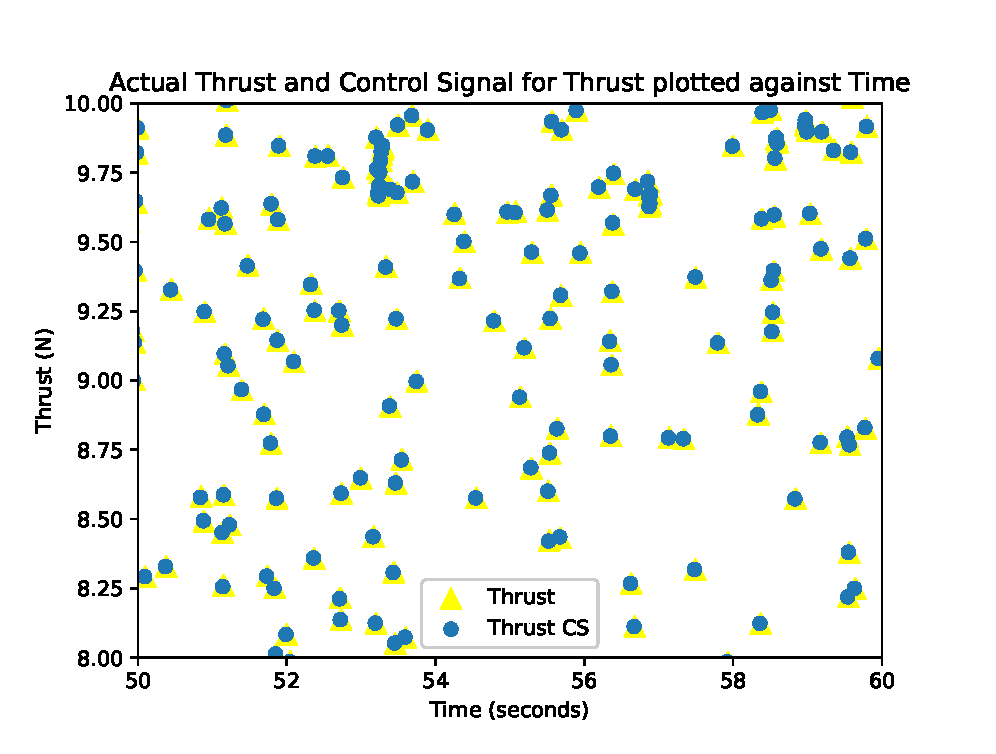
\includegraphics[height=5.5cm,keepaspectratio]{img/thrust_plot.eps}
        \caption{Actual thrust and control signal for thrust plotted against time}
        \label{fig:thrust_plot}
    \end{minipage}
    \hfill
    \begin{minipage}[b]{0.45\textwidth}
        \centering
        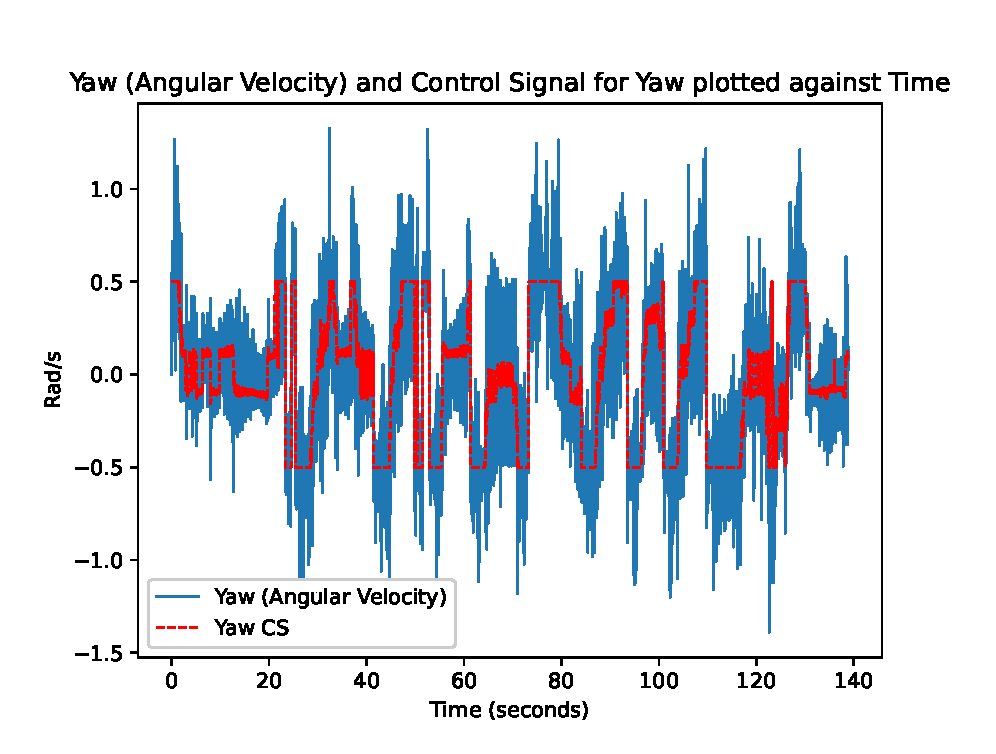
\includegraphics[height=5.5cm,keepaspectratio]{img/yaw_plot.eps}
        \caption{Yaw (angular velocity) and Control Signal for Yaw plotted against time}
        \label{fig:yaw_plot}
    \end{minipage}
\end{figure}
\begin{figure}[H]
    \centering
    \begin{minipage}[b]{0.45\textwidth}
        \centering
        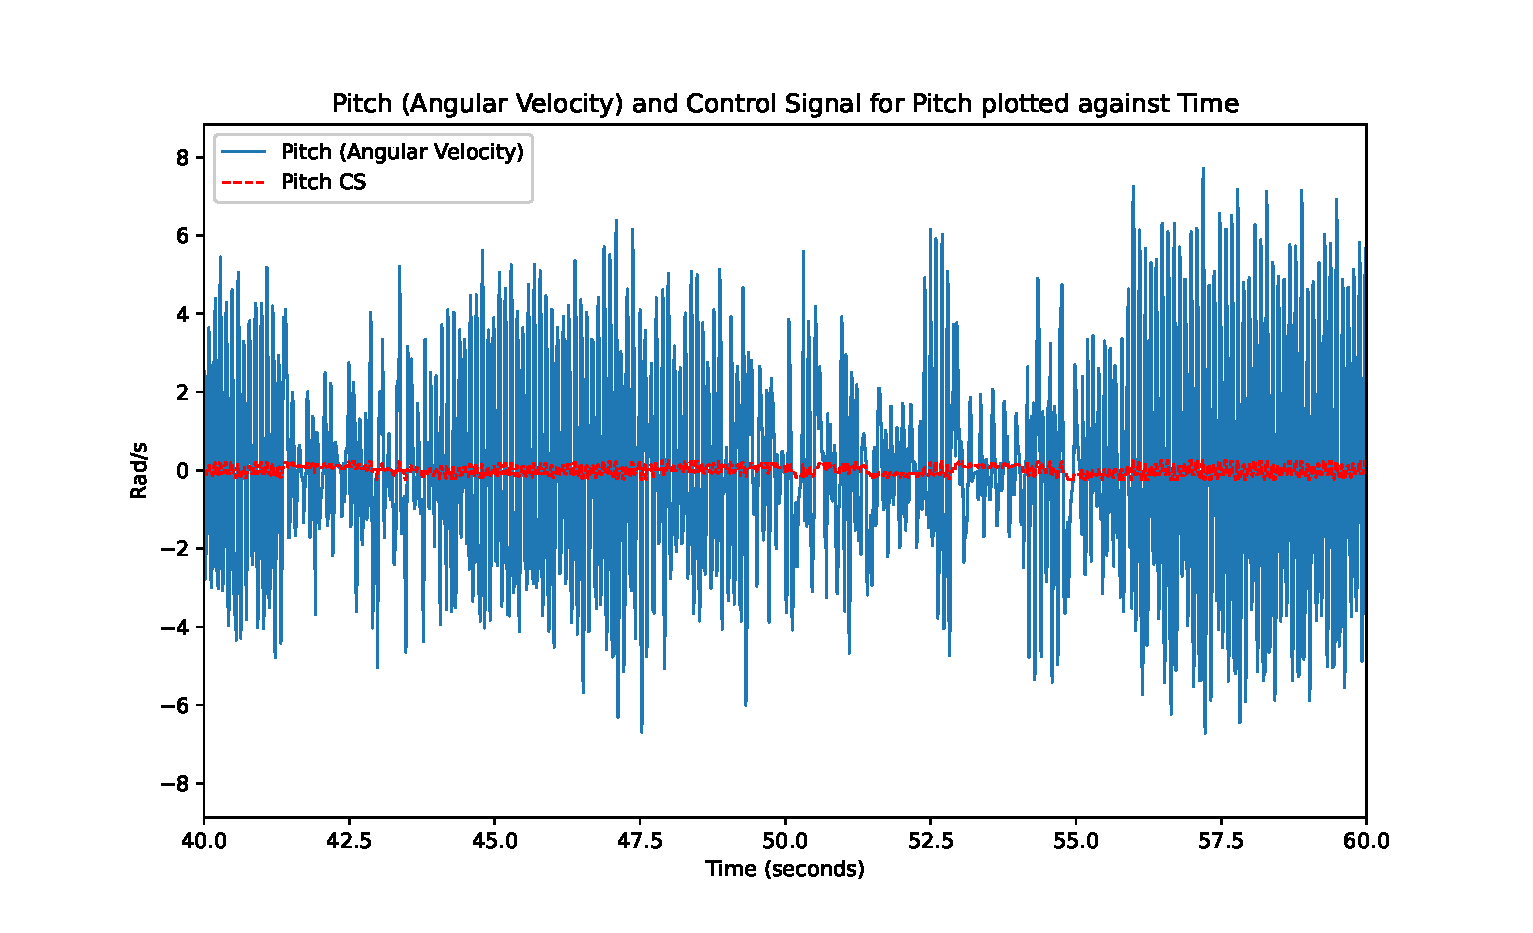
\includegraphics[height=5.5cm,keepaspectratio]{img/pitch_plot.eps}
        \caption{Pitch (angular velocity) and Control Signal for Pitch plotted against time}
        \label{fig:pitch_plot}
    \end{minipage}
    \hfill
    \begin{minipage}[b]{0.45\textwidth}
        \centering
        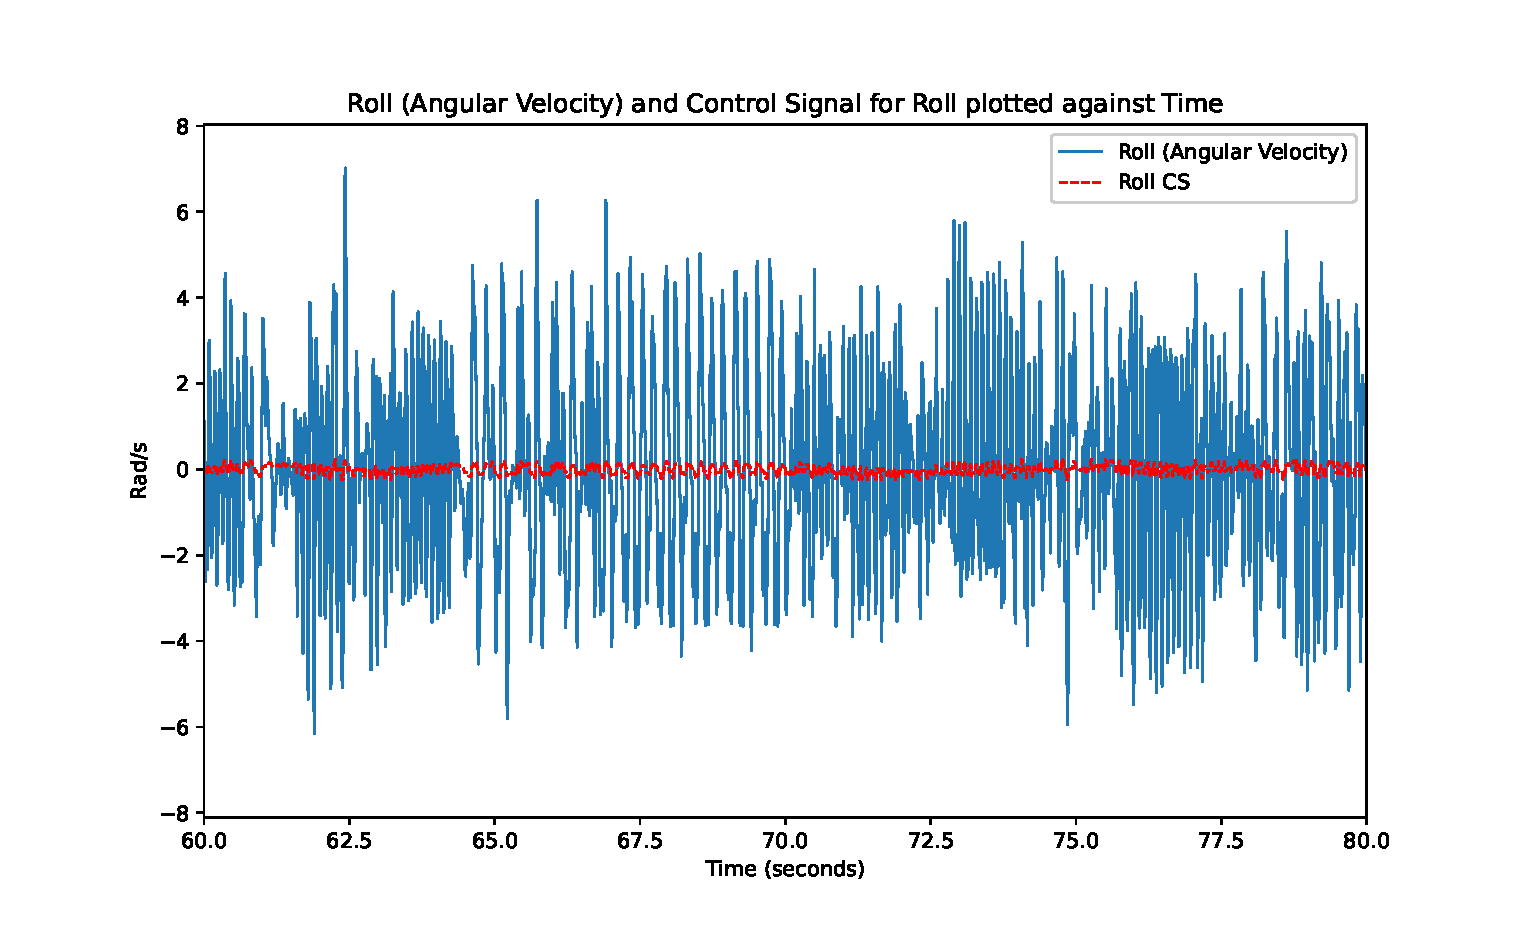
\includegraphics[height=5.5cm,keepaspectratio]{img/roll_plot.eps}
        \caption{Roll and Control Signal for Roll plotted against time}
        \label{fig:roll_plot}
    \end{minipage}
\end{figure}
\begin{figure}[H]
    \centering
    \begin{minipage}[b]{0.45\textwidth}
        % empty minipage
    \end{minipage}
    \hfill
    \begin{minipage}[b]{0.45\textwidth}
        \centering
        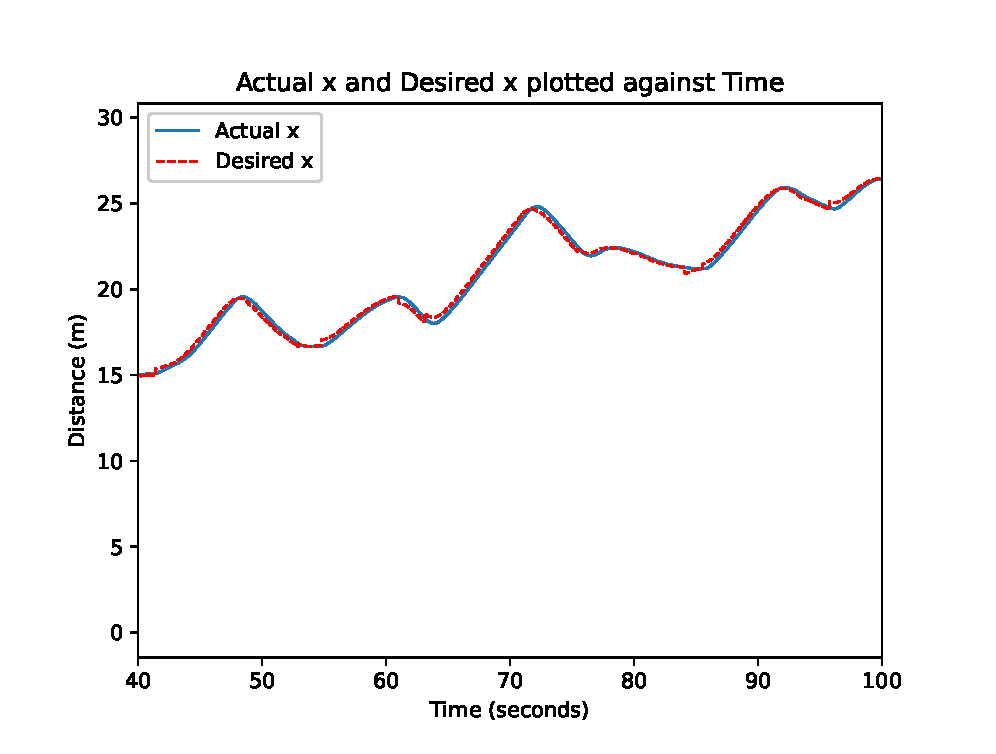
\includegraphics[height=5.5cm,keepaspectratio]{img/x_plot.eps}
        \caption{Actual position x and desired position x plotted against time.}
        \label{fig:x_plot}
    \end{minipage}
    \hfill
    \begin{minipage}[b]{0.45\textwidth}
        % empty minipage
    \end{minipage}
\end{figure}
Figure \ref{fig:thrust_plot}  shows that the actual thrust value and the control signal are almost equivalent in most cases. Figure \ref{fig:yaw_plot} shows the yaw control signal is often discrete at either \SI{0.5}{\radian\per\second} or \SI{-0.5}{\radian\per\second}, which makes intuitive sense due to yaw representing a significant alteration in the drone’s direction of travel. Figures \ref{fig:pitch_plot}  and \ref{fig:roll_plot} are similar and show that the pitch and roll values are subject to more continuous variation. As seen from Figure \ref{fig:x_plot} the actual $x$ value for the drone closely follows the desired $x$ value as expected. The difference between these values is a key indication of the performance of the drone and will be discussed in Chapter \ref{chapter5}. 
\section{Feature Selection and Engineering} \label{feature selection}
Feature selection and engineering is an important step when training any machine learning system. 

Despite time, $t$, being part of the set of inputs shown in Table \ref{tab:inputsOutputs}, it is not used by the drone and is not relevant to the training of the drone, the time variable was removed. This reduced the number of inputs down to 17. Due to the Simulink drone model using all the remaining 17 inputs in its controller, any feature selection and engineering would mean the model must be altered accordingly, such that the controller is fed the same inputs as the neuro-fuzzy controller is trained on. Therefore, only limited feature engineering and selection was carried out.  

Absolute measures that were not relative to the drone's movement are not useful to the learning based system. As a result, desired position and actual position both are absolute measures therefore this information was not helpful for the neuro-fuzzy controller. Instead, the difference between the desired position and actual position is of relevance. Therefore, the following feature engineering was performed: 
\begin{align}
    x_{\textrm{desired}} - x_{\textrm{actual}} & = x_{\textrm{desired change}}\\
    y_{\textrm{desired}} - y_{\textrm{actual}} & = y_{\textrm{desired change}}\\
    z_{\textrm{desired}} - z_{\textrm{actual}} & = z_{\textrm{desired change}}
\end{align}
This resulted in the number of inputs further decreasing from 17 to the 14. Reducing the number of inputs further would require appropriate adjustments to the Simulink model which could lead to computational inefficiencies. Despite this, it was important to check if there were any unnecessary features in order to not waste computational power. The filter feature selection method was applied to check this. This method is very useful for machine learning models with numerical inputs and outputs. The filter feature selection method chosen was the Pearson Correlation Coefficient method where the Pearson coefficients were analysed and a heatmap of the correlation between the features was created. This can be seen in Figure \ref{fig:zain6}. The features with highest correlation were the velocities in the $x$, $y$ and $z$ direction and their corresponding desired changes in the $x$, $y$ and $z$ directions. As found in literature, a correlation coefficient greater than 0.85 demonstrates a strong correlation and consequently should be removed \cite{654654}. Since we did not have any features with correlation coefficients greater than 0.85, no features were removed and all were deemed to provide relevant information to the fuzzy inference system.
\begin{figure}[H]
    \centering
    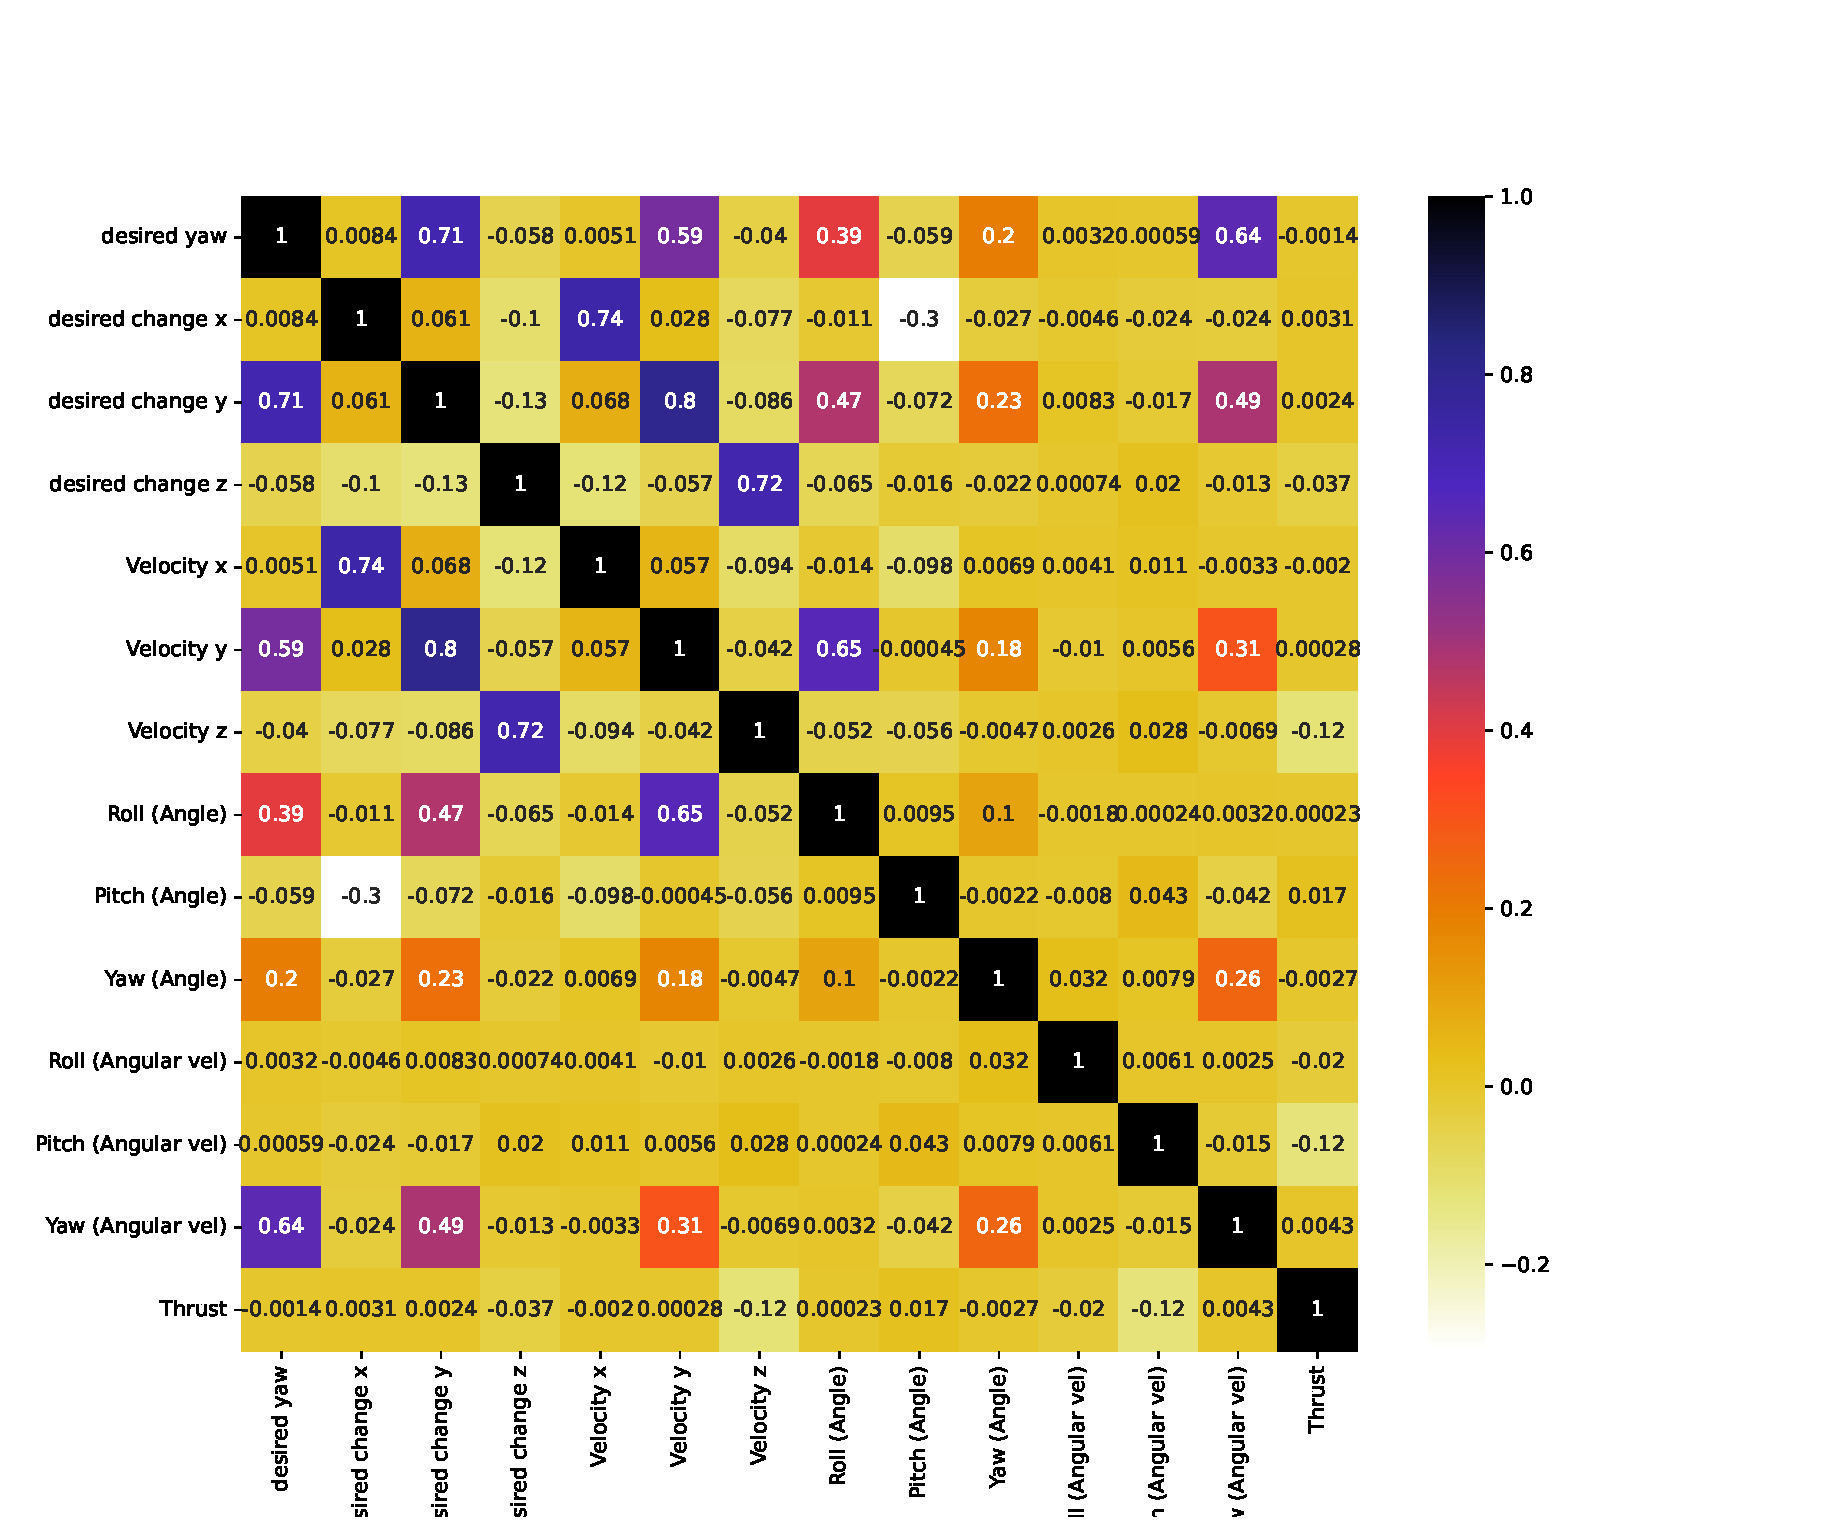
\includegraphics[width = 0.7\textwidth]{img/pearson.eps}
    \caption{Pearson correlation coefficient heatmap.}
    \label{fig:zain6}
\end{figure} 
\section{ANFIS Configuration}
There may be instances of natural phenomena that inherently possess a degree of indeterminacy, making them difficult to accurately model without embracing some level of non-probabilistic uncertainty. One technique to address this ambiguity is the application of fuzzy logic. Fuzzy values or fuzzy sets do not adhere to strictly defined numerical limits, often referred to as sharp boundaries. Rather, these boundaries tend to gradually fade in the context of fuzzy sets. In general, a Sugeno-type inference system is proposed, with the resultant parameters of the fuzzy rules presented as a polynomial function: 
\begin{align}
    &\texttt{if } X \subset A \And Y \subset B\\
    &\texttt{then } Z = f\left(X,Y\right)\\
    &\texttt{where } f\left(X,Y\right) = pX + qY + r
\end{align}
For the purpose of simplicity, consider a fuzzy inference system with two inputs labelled $X$ and $Y$, as well as a single output labelled $Z$. It is assumed that the rule base consists of two fuzzy if-then rules organised in accordance with Takagi and Sugeno's type \cite{TAKAGI198355}.

Rule 1:
\begin{align}
    &\texttt{if } X = A_1 \And Y = B_1\\
    &\texttt{then } f_1 = p_1X + q_1 Y + r_1
\end{align}
Rule 2:
\begin{align}
    &\texttt{if } X = A_2 \And Y = B_2\\
    &\texttt{then } f_2 = p_2X + q_2 Y + r_2
\end{align}
In linguistic terms, each rule is assigned a distinct weight that contributes to the generation of the output $f$. This output is determined based on the conjunction (AND) rule. The design parameters, namely $p$, $q$, $r$ are utilised during the training process.
\subsection{Training, Validation and Test Data}
Before splitting the dataset into training, validation and test subsets the dataset was randomly shuffled. As this dataset is ``class-balanced'' i.e. it has the same number of samples for every feature, random sampling has no drawbacks and is optimal in order to prevent bias when training the ANFIS model. 
There are three common data splits:
\begin{itemize}
    \item 60\% train, 20\% validate, 20\% test
    \item 70\% train, 15\% validate, 15\% test
    \item 80\% train, 10\% validate, 10\% test
\end{itemize}
A large training dataset is helpful to train the ANFIS, however the validation and test datasets are also important to test the ANFIS in other drone scenarios. Therefore, the widely used: 70\% train, 15\% validate, 15\% test split was chosen, which also has evidence of performing best for large datasets \cite{zain1}. As a result, the sizes of the datasets were as shown in Table \ref{tab:zain1}.
\begin{table}[H]
    \centering
    \begin{tabular}{@{}ll@{}}
        \toprule
        \textbf{Dataset} & \textbf{Sample size} \\
        \midrule
        Training & 353,533\\
        Validation & 75,761\\
        Test & 75,761\\
        \bottomrule
    \end{tabular}
    \caption{Size of datasets.}
    \label{tab:zain1}
\end{table}
\subsection{Fuzzy Sets and Membership Functions}\label{membership function}
Fuzzy sets are the foundation of the ANFIS structure and are denoted by the following equation: 
\begin{gather}
A = \left\{ \left(x,\; \mu_A\left(x\right)\right) \;|\; x \in X \right\}
\end{gather}
Where $A$ is the fuzzy set, $X$ is a collection of objects, generically characterised by $x$ and $\mu_A(x)$ is the characteristic function of $A$. The fuzzy set is simply an extension of a classical set where the characteristic function can take any values between 0 and 1. If $\mu_A(x)$ was restricted to discrete values of either 0 or 1, $A$ would be a classical set. Therefore, fuzzy sets refer to a degree of uncertainty or degree of ``membership'' of values within the set. Membership functions can take various forms and can alter the accuracy of the output of the ANFIS. Figure \ref{fig:types_mf} shows the different ways the membership functions can be characterised. 
\begin{figure}[H]
    \centering
    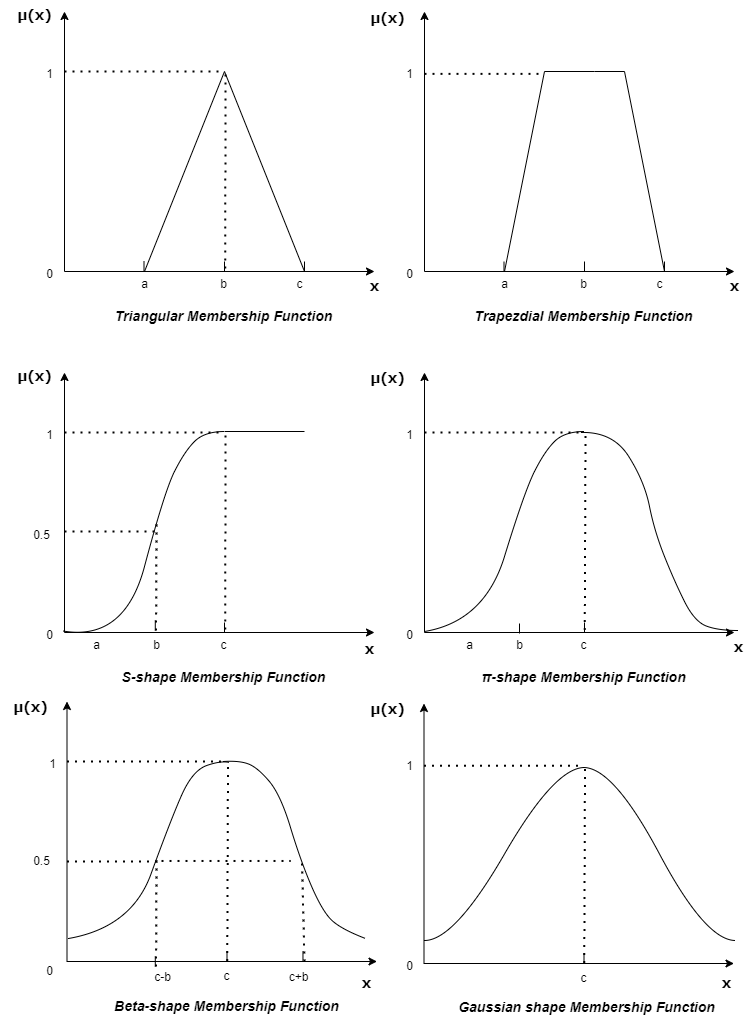
\includegraphics[width = 0.7 \textwidth]{img/membershipfunctions.png}
    \caption[Graphs of various types of fuzzy logic membership functions.]{Graphs of various types of fuzzy logic membership functions \cite{zain5}.}
    \label{fig:types_mf}
\end{figure}
Figure \ref{fig:types_mf} shows the shapes every membership function $\mu$ can take. Examples include suitable triangular or trapezoidal functions as well as Gaussian and bell-shaped functions. Considering the differential nature of gradient descent, it is recommended to utilise differentiable alternatives like Gaussian, sigmoidal, or generalised bell functions. The premise parameters, also known as antecedent parameters, are variables that shape these functions and undergo modifications during the back-propagation error correction process. Through findings from the literature review and the functions offered by MATLAB, the optimal membership functions for the features was chosen to be the Gaussian membership function. As a result, the Gaussian membership function was used to map all the inputs. It is important to note that these membership functions define the degree of membership of the input variables for only the specified range of inputs, i.e. anything outside the universe of $X$ will have a membership function of zero. Consequently, an ANFIS structure cannot extrapolate.  
\subsection{ANFIS Methods}
There are two different methods of designing an ANFIS: a Sugeno ANFIS and a Mamdani ANFIS. In the context of a drone control system, a Mamdani ANFIS could use several linguistic labels for each input variable (such as ``high'' or ``low'' altitude), with each label associated with a membership function. The output is also fuzzy in nature and defuzzification is needed to get a crisp output. This method is intuitively appealing and can be used to capture expert knowledge about how the drone should respond in different scenarios. However, it may be computationally intensive due to the requirement of defuzzification, which might limit its real-time applicability in high-speed scenarios, such as drone control. 

On the other hand, the Sugeno ANFIS method, instead of outputting a fuzzy set, produces a weighted average as its output. The Sugeno method typically requires less computational resources because the output is a polynomial function of the input variables, avoiding the need for defuzzification. In a drone control system, this could be advantageous when rapid responses to changing conditions are necessary, such as when the drone is manoeuvring in a complex environment. However, Sugeno systems can be more challenging to design and interpret because they don't use linguistic variables in the same way as Mamdani systems.

For the application of drone control, where computational efficiency and measurable, crisp outputs are used, the Sugeno design is likely to be the optimal ANFIS configuration. 

\subsection{ANFIS Types}
Type-1 and Type-2 ANFIS and they differ in how they handle uncertainty in the system.The difference between Type-1 and Type-2 fuzzy logic membership function is shown in Figure \ref{fig:type}.
The Type-1 ANFIS represents the more conventional and frequently used variant, employing standard fuzzy logic principles derived from Type-1 fuzzy sets. The degree of membership of an element in a fuzzy set is described by a membership function which can range between 0 and 1. This can be seen in Figure \ref{fig:type} with a single line indicating a crisp value relating $x_i$ (the range of possible values for a variable) and $\mu(x_i)$) representing the degree of membership for each value in the fuzzy set. In such a system, a variable's degree of membership to a fuzzy set is precise and ascertainable, making it effective for situations with explicit control rules. For instance, in the management of a drone control system, a Type-1 ANFIS, could contain distinct protocols dictating the drone's actions upon reaching specific altitudes or facing particular wind speeds. It delivers a single, definitive output for each respective input, assuming the same underlying conditions. Nevertheless, the Type-1 ANFIS may encounter difficulties when grappling with uncertainties or in the presence of noisy data or fluctuating environmental conditions - situations that are frequently encountered in real-world scenarios of drone navigation and control.

Type-2 FIS, on the other hand, have a fuzzy degree of membership i.e. can take values within a range. This is shown in Figure \ref{fig:type} where the shading values represent the uncertainty in the degree of membership for the different values of the variable. Type-2 FIS can be used for handling uncertain and vague input data, such as decision making in complex environments. This proves especially advantageous in intricate, volatile environments characterised by substantial uncertainty or noise, as it permits the system to assimilate and process this uncertainty instead of simply malfunctioning or generating an incorrect result.

For a drone control application, Type-2 ANFIS could be valuable in circumstances characterised by significant uncertainty or swift alterations in conditions, such as during a storm, or in regions with erratic wind flows. However, the literature review suggested that the level of uncertainty in the data set will be a key indicator of which ``type'' will be more effective. From the plots for the thrust and yaw in Figures \ref{fig:thrust_plot}\ref{fig:yaw_plot}, the optimal ANFIS configuration is likely to be a Type-1 design due to the minimal uncertainty. From the plots for the roll and pitch outputs in Figures \ref{fig:roll_plot} and \ref{fig:pitch_plot}, the uncertainty is higher and therefore a Type-2 design could be better in these cases. 
\begin{figure}[H]
    \centering
    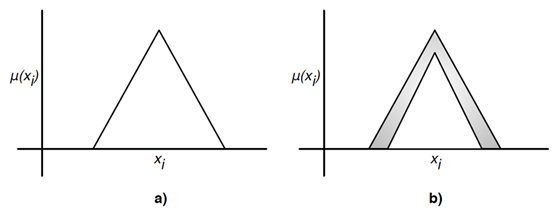
\includegraphics[width = 0.7 \textwidth]{img/Picture9.png}
    \caption[Graphs of fuzzy logic membership functions: a) Type-1; b) Type-2.]{Graphs of fuzzy logic membership functions: a) Type-1; b) Type-2 \cite{boxi8}.}
    \label{fig:type}
\end{figure}
\subsection{ANFIS Parameters Decision Making}
In order to determine the best design for the ANFIS for each output variable, we used the approach outlined in Figure \ref{fig:flow_fis}.
\begin{figure}[H]
    \centering
    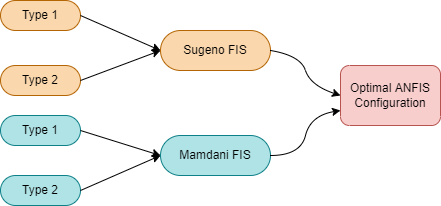
\includegraphics[width = 0.7\textwidth]{img/5.5drawio.png}
    \caption{Flowchart for ANFIS Configuration Decision making}
    \label{fig:flow_fis}
\end{figure}
The performance metric used to make these decisions was the Root Mean Square Error (RMSE) of the ANFIS. The RMSE is calculated in the following way:
\begin{equation}
\text{RMSE} = \sqrt{\frac{1}{n} \sum_{i=1}^{n} (y_i - \hat{y}_i)^2}
\end{equation}
Where $n$ is the total number of data points, $y_i$ is the actual value and $\hat{y}_i$ is the predicted value. The RMSE is a commonly used metric for measuring the differences between predicted and observed values. A lower RMSE value signifies a model with better predictive accuracy and there is a smaller difference between the actual values and the predicted values. 
\section{Implementation of Fuzzy Logic Controller}
A hybrid PID-ANFIS controller was implemented in Simulink. This approach checks each input at every time-step, to ensure that it is within the range of the FIS. If it is not, it will revert to the original PID controller. This is shown in Figure \ref{fig:Hybrid Control}. Although a hybrid PID-ANFIS controller was used, for clarity in results, this will be referred to as an ANFIS controller. This duality with PID control ensures the ANFIS controller is able to operate at every state, at the cost of program complexity and greater computational cost. The reason for this approach is because the fuzzy logic controller does not extrapolate due to the nature of the membership functions, as discussed in Section \ref{membership function}. If it receives an input that is outside of the original range of the training set, then the fuzzy logic controller is unable to provide an output. Although the Gaussian membership function is used, the membership function is actually limited by the range of the training data, contrary to what its name may suggest.
\begin{figure}[H]
    \centering
    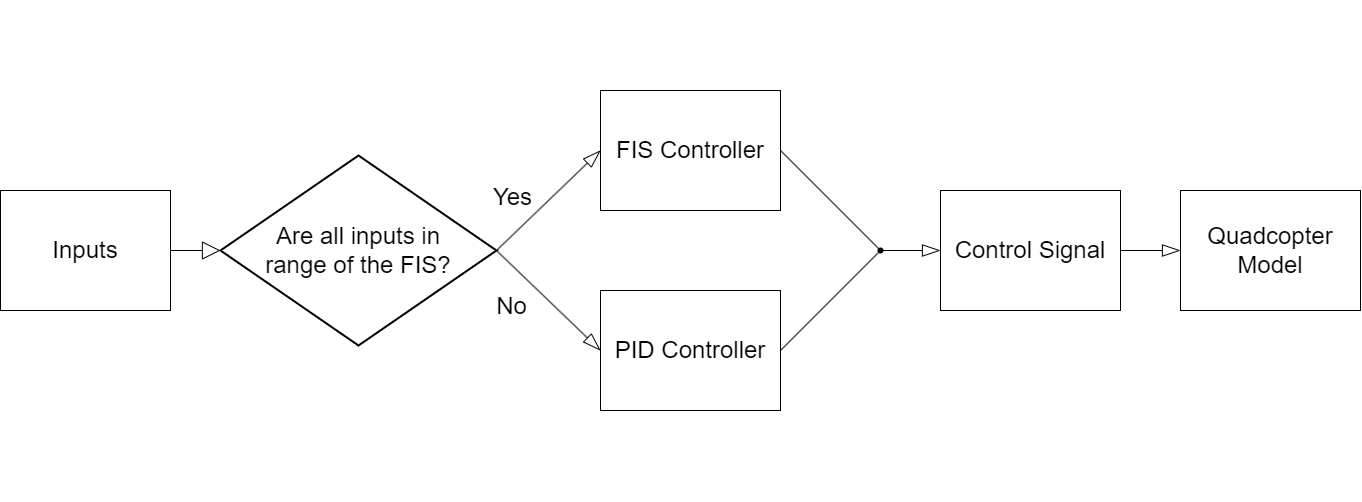
\includegraphics[width = \textwidth]{./img/hybrid_control.png}
    \caption{Flow chart for whether the FIS or PID controller will be used.}
    \label{fig:Hybrid Control}
\end{figure}
This was especially apparent when using the absolute position of the drone in the simulation environment, as it is nearly impossible to have a data-set encompassing all possible positions of the drone. To overcome this, the feature engineering of desired change in position, obtained by finding the difference between the desired position and current position, discussed in Section \ref{feature selection}, was used. As mentioned, this finds the relative position the drone wants to move to, while also reducing the number of inputs.

However, there were still edge cases where the inputs were not within the range of the fuzzy logic controller. This may be due to edge cases that were not covered in the training data, or new states that arise from the difference in behaviour of the fuzzy logic controller. This led to the implementation of the hybrid controller.

Another limitation is that MATLAB can only use neuro-adaptive learning methods to tune Type-1 Sugeno FIS with a single output as per MathWorks documentation. A workaround is that it is possible to tune the FIS, then convert it to another type, keeping the tuning. Tuning is an important step in FIS design, as it is used to optimise the membership functions. This is to obtain the membership functions which minimises the training error. This meant the options for controller design was very limited. Even though this was the case, various configurations were designed and tested even if some cannot be tuned. Two configurations for the fuzzy logic controller were made, one with four separate controllers, each with a single control signal output, with parameter selection and tuning; and one combined controller without parameter selection and tuning. These are shown in Figure \ref{fig:fis comparison}. This also provided insight on the improvement between a FIS with and without tuning. Through small simulation testing, the single controller configuration (Left of Figure \ref{fig:fis comparison}) was judged to be much less capable than the four seperate controller configuration, due to the inability to tune a single ANFIS for multiple outputs. 
\begin{figure}[H]
    \centering
    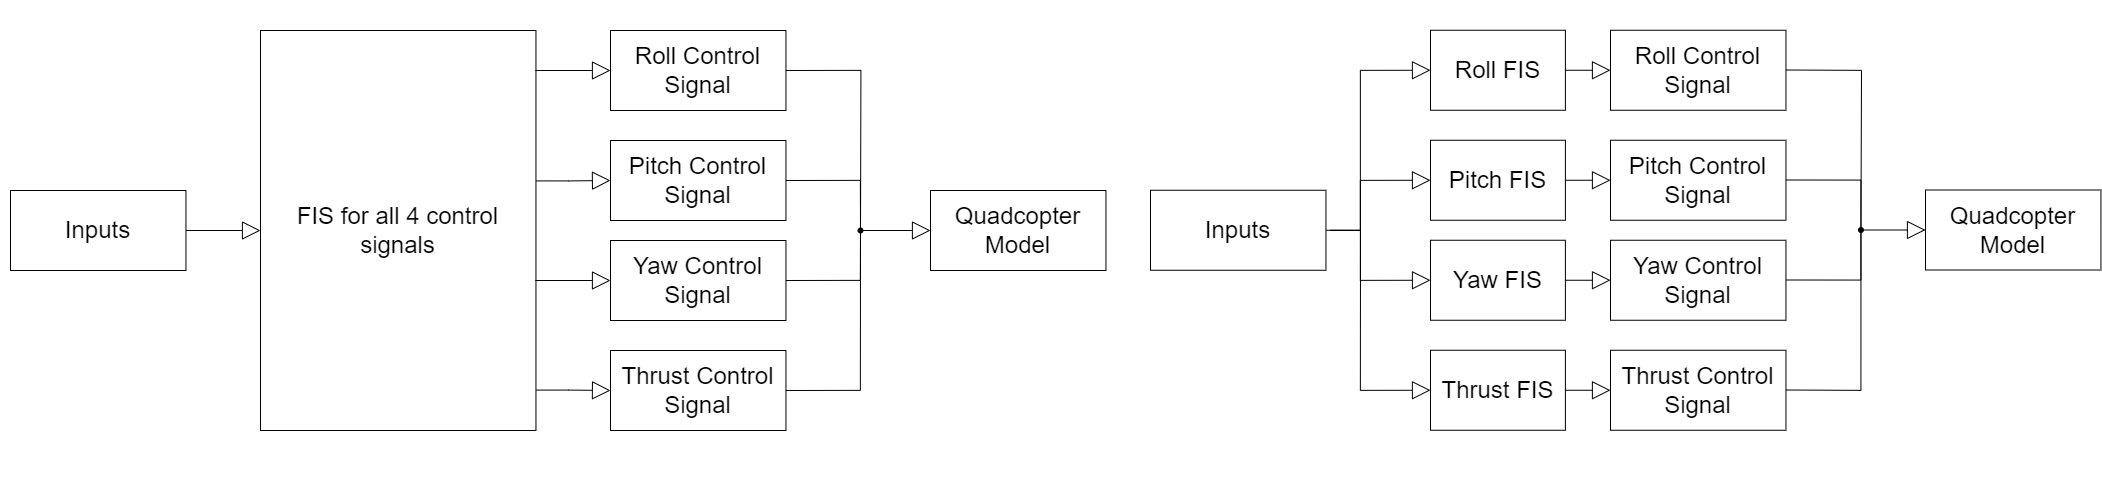
\includegraphics[width = \textwidth]{./img/fis_comparison.png}
    \caption{Left: Controller with single FIS and four outputs. Right: Four separate controllers with one output for each control signal.}
    \label{fig:fis comparison}
\end{figure}
\chapter{Results and Discussion}\label{chapter5}
\section{ANFIS Configuration}
\subsection{ANFIS Tuning}
As mentioned in Chapter 4, the tuning for each controller was carried out on the Sugeno Type 1 configuration and after the ANFIS had been tuned it was converted to Mamdani and Type 2 for testing. The validation dataset was used for validation tuning. MATLAB’s Fuzzy Logic Designer runs a specified number of iterations and looks to minimise the RMSE. At the end of the tuning, it chooses the combination which minimises the validation error. The results from the validation tuning can be seen in Figures \ref{fig:roll_tuning}, \ref{fig:pitch_tuning}, \ref{fig:yaw_tuning} and \ref{fig:thrust_tuning}. The results show that all the outputs' validation RMSEs closely followed the training RMSE except from pitch which had a slight difference. This shows that the tuning of membership functions was successful in reducing the training error, whilst ensuring the validation error was minimised. This was particularly effective for the tuning of the thrust ANFIS where the training error was reduced by 12.5\%. 
\begin{figure}[H]
    \centering
    \begin{minipage}[b]{0.45\textwidth}
        \centering
        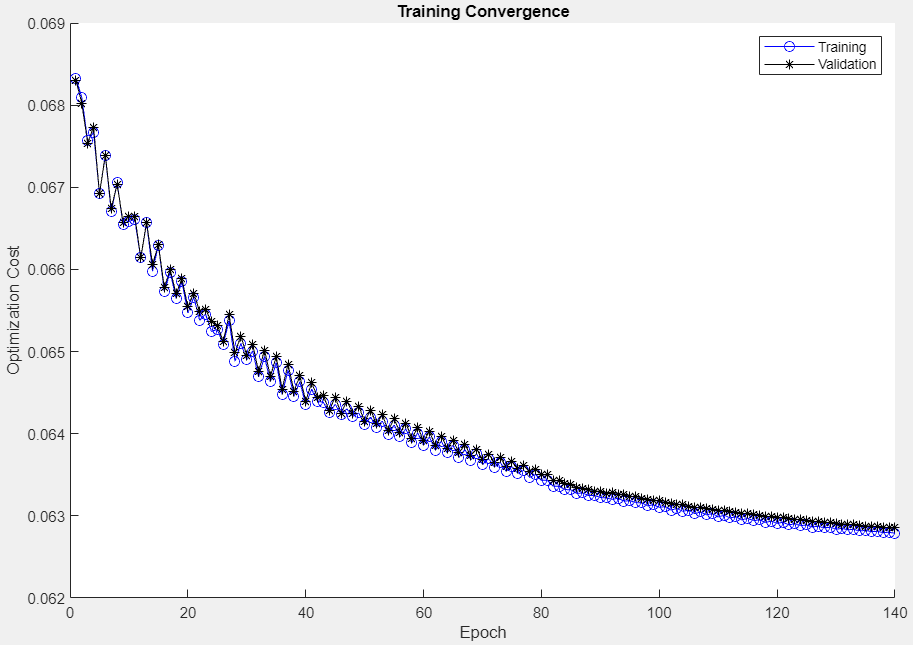
\includegraphics[height=5.5cm,keepaspectratio]{img/roll_tuning.png}
        \caption{Training convergence plot for Roll to find the iteration with the minimum training RMSE and validation RMSE}
        \label{fig:roll_tuning}
    \end{minipage}
    \hfill
    \begin{minipage}[b]{0.45\textwidth}
        \centering
        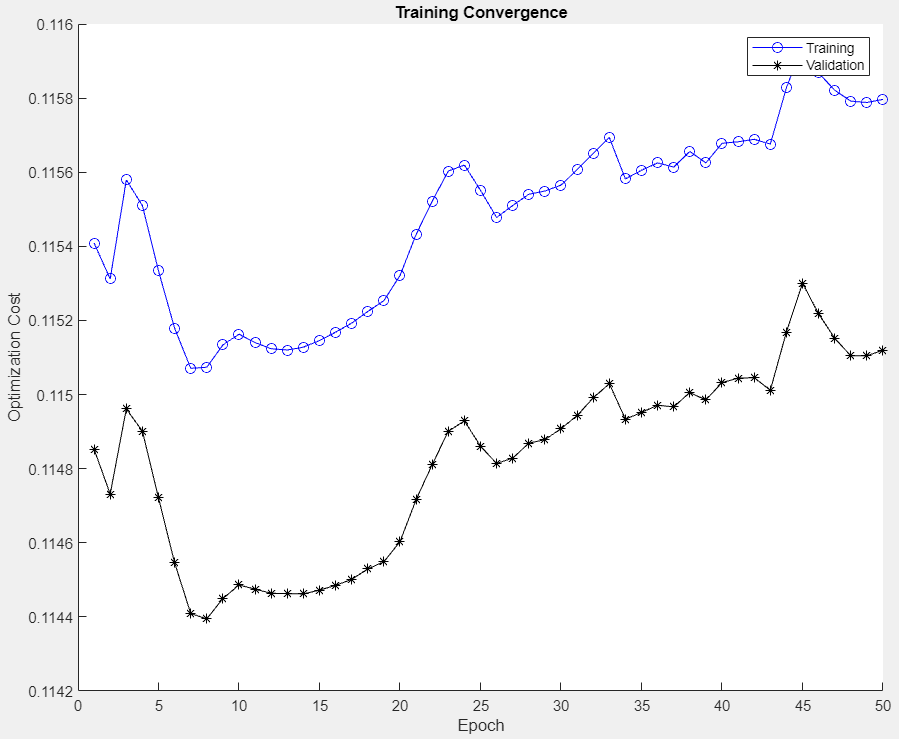
\includegraphics[height=5.5cm,keepaspectratio]{img/pitch_tuning.png}
        \caption{Training convergence plot for Pitch to find the iteration with the minimum training RMSE and validation RMSE}
        \label{fig:pitch_tuning}
    \end{minipage}
\end{figure}
\begin{figure}[H]
    \centering
    \begin{minipage}[b]{0.45\textwidth}
        \centering
        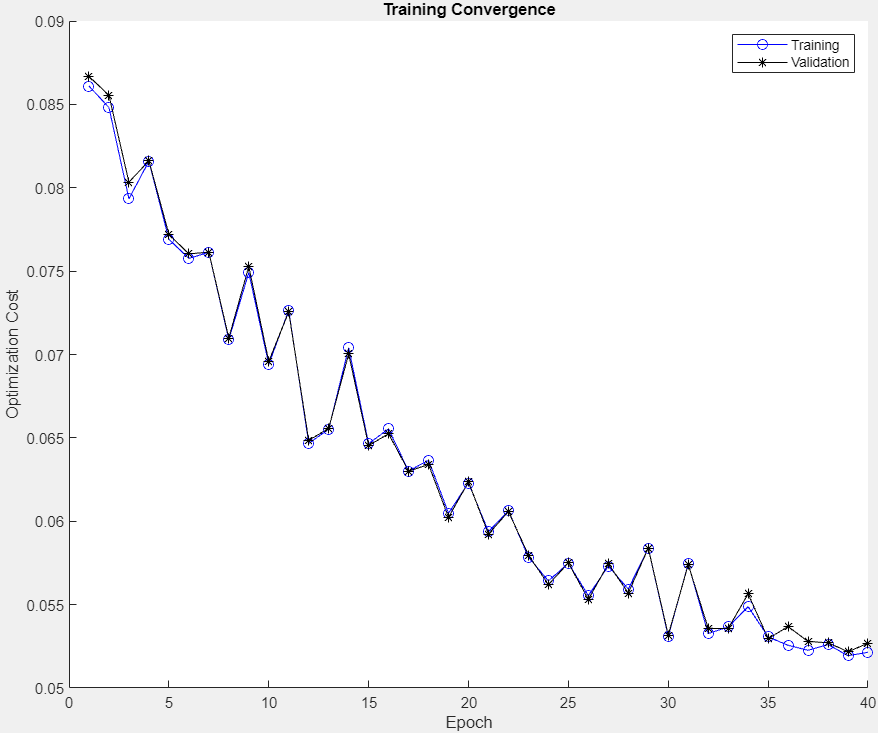
\includegraphics[height=5.5cm,keepaspectratio]{img/yaw_tuning.png}
        \caption{Training convergence plot for Yaw to find the iteration with the minimum training RMSE and validation RMSE}
        \label{fig:yaw_tuning}
    \end{minipage}
    \hfill
    \begin{minipage}[b]{0.45\textwidth}
        \centering
        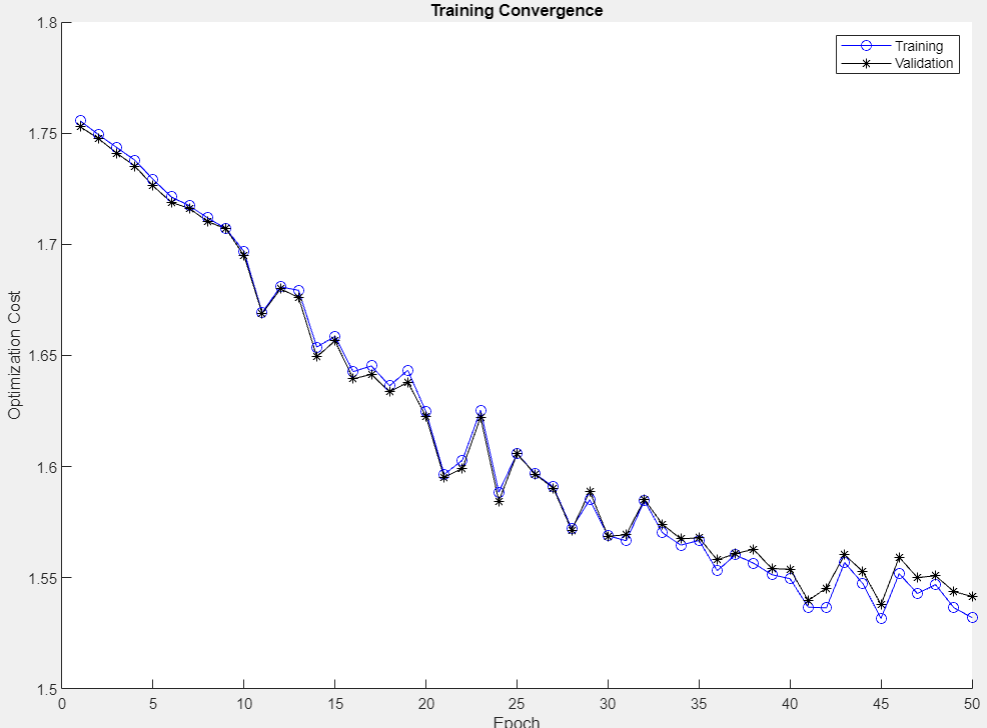
\includegraphics[height=5.5cm,keepaspectratio]{img/thrust_tuning.png}
        \caption{Training convergence plot for Thrust to find the iteration with the minimum training RMSE and validation RMSE}
        \label{fig:thrust_tuning}
    \end{minipage}
\end{figure}
The results from tuning are summarised in Table \ref{tab:results1}. The number of epochs represents the number of passes through the training dataset. As seen from Table \ref{tab:results1} and Figures \ref{fig:roll_tuning}, \ref{fig:pitch_tuning}, \ref{fig:yaw_tuning},\ref{fig:thrust_tuning}, the number of epochs were adjusted in order to allow the tuning process to reach the minimum validation error and corresponding training error. 
\begin{table}[H]
\centering
    \begin{tabular}{@{}lllll@{}}
        \toprule
                                      & Roll    & Pitch  & Yaw     & Thrust \\ \midrule
        Number of   epochs            & 140     & 50     & 60      & 50     \\
        Number of   tuning parameters & 731     & 464    & 1075    & 989    \\
        Minimum   Validation RMSE     & 0.06285 & 0.1151 & 0.04589 & 1.5380 \\
        Training RMSE                 & 0.06279 & 0.1144 & 0.04850 & 1.5317 \\ \bottomrule
    \end{tabular}
    \caption{Validation tuning results.}
    \label{tab:results1}
\end{table}
\subsection{ANFIS Parameter Selection}
After tuning, the ANFIS for each output was converted to Mamdani and Type-2 systems and then the test data was compared to the training data. The results for each `Type' were first obtained, in line with the methodology given in Figure \ref{fig:flow_fis}. RMSE was used as the performance metric to compare the configurations. The results for comparing each `Type' for each output can be seen in Table \ref{tab:results2}, with the plots in the Appendix (Figures \ref{fig:roll_type}, \ref{fig:pitch_type}, \ref{fig:yaw_type}, \ref{fig:thrust_type}). As seen, the optimal Type for all Sugeno ANFIS configurations was Type-1 in all cases. For the Mamdani configurations, the optimal type for the Roll and Yaw outputs was Type-2 and for the Pitch and Thrust outputs was Type-1.
\begin{table}[H]
\centering
    \begin{tabular}{@{}lllllllll@{}}
        \toprule
        & \multicolumn{2}{c}{Roll} & \multicolumn{2}{c}{Pitch} & \multicolumn{2}{c}{Yaw} & \multicolumn{2}{c}{Thrust} \\
        & Sugeno     & Mamdani     & Sugeno      & Mamdani     & Sugeno     & Mamdani    & Sugeno      & Mamdani      \\
        \midrule
        Optimal   “Type” & Type-1     & Type-2      & Type-1      & Type-1      & Type-1     & Type-1     & Type-1      & Type-1      \\
        \bottomrule
    \end{tabular}
    \caption{Results from comparing each configuration ``type'' for each output variable.}
    \label{tab:results2}
\end{table}
Following this, the Sugeno and Mamdani configurations were compared using the optimal ``Type'' for each (as per Table \ref{tab:results2}) and using RMSE as the performance metric for both systems. These can be seen in Figures \ref{fig:roll_SvM}, \ref{fig:pitch_SvM}, \ref{fig:yaw_SvM} and \ref{fig:thrust_SvM}. The results show that the Mamdani ANFIS has a consistent range of prediction errors whereas Sugeno fluctuate more. This is due to the Sugeno design producing crisp values for the membership function whereas Mamdani uses fuzzy sets for its membership function, meaning the Mamdani has less fluctuation in its errors. Despite this, as seen from the figures, Sugeno Type-1 was the best configuration for all four outputs as it provided the minimum RMSE in all cases. This followed what was found in the literature review as Sugeno Type-1 FIS are known for its direct, crisp output and better computational efficiency, whereas Mamdani Type-2 FIS are generally better in applications where human reasoning and non-crisp outputs are preferred \cite{zain3,boxi12}. Therefore, in the context of a drone application, where all four outputs (roll, pitch, yaw and thrust) are to be crisp and have measurable values, it was logical that the Sugeno Type-1 configuration was the best. 
\begin{figure}[H]
    \centering
    \begin{minipage}[b]{0.45\textwidth}
        \centering
        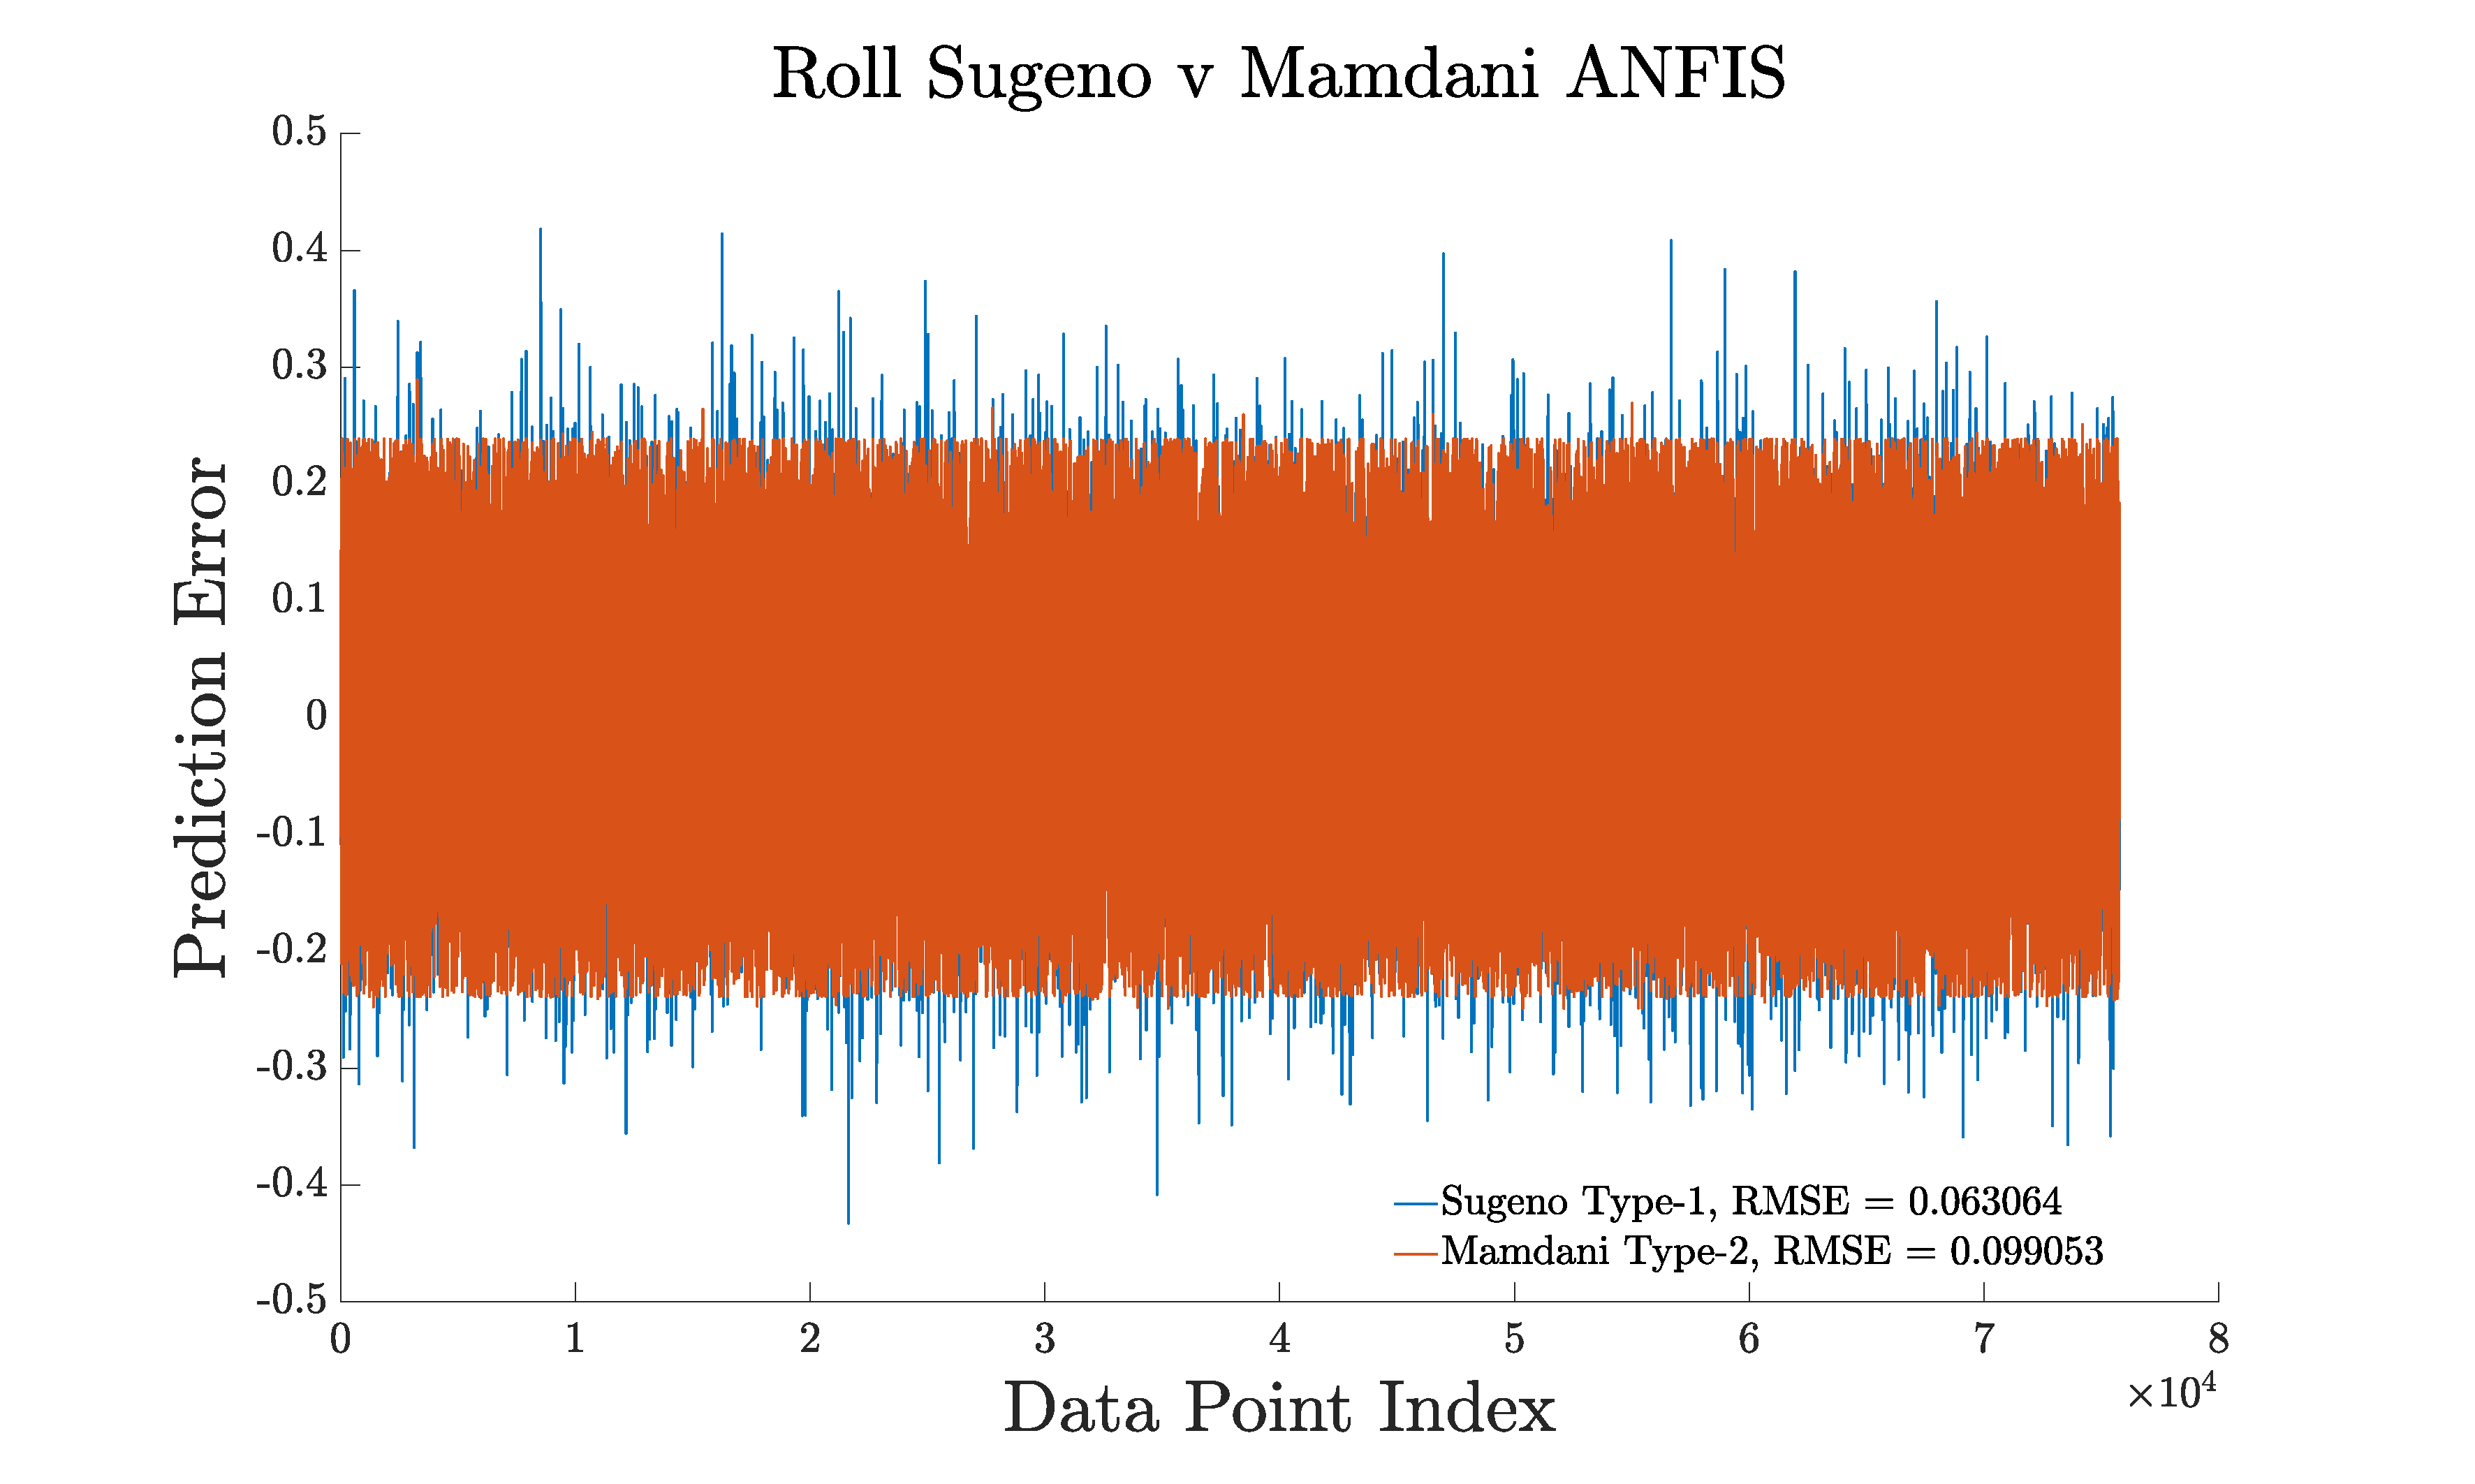
\includegraphics[height=5cm,keepaspectratio]{img/Roll SvM.pdf}
        \caption{RMSE results for the best Sugeno and Mamdani Configurations for Roll Output}
        \label{fig:roll_SvM}
    \end{minipage}
    \hfill
    \begin{minipage}[b]{0.45\textwidth}
        \centering
        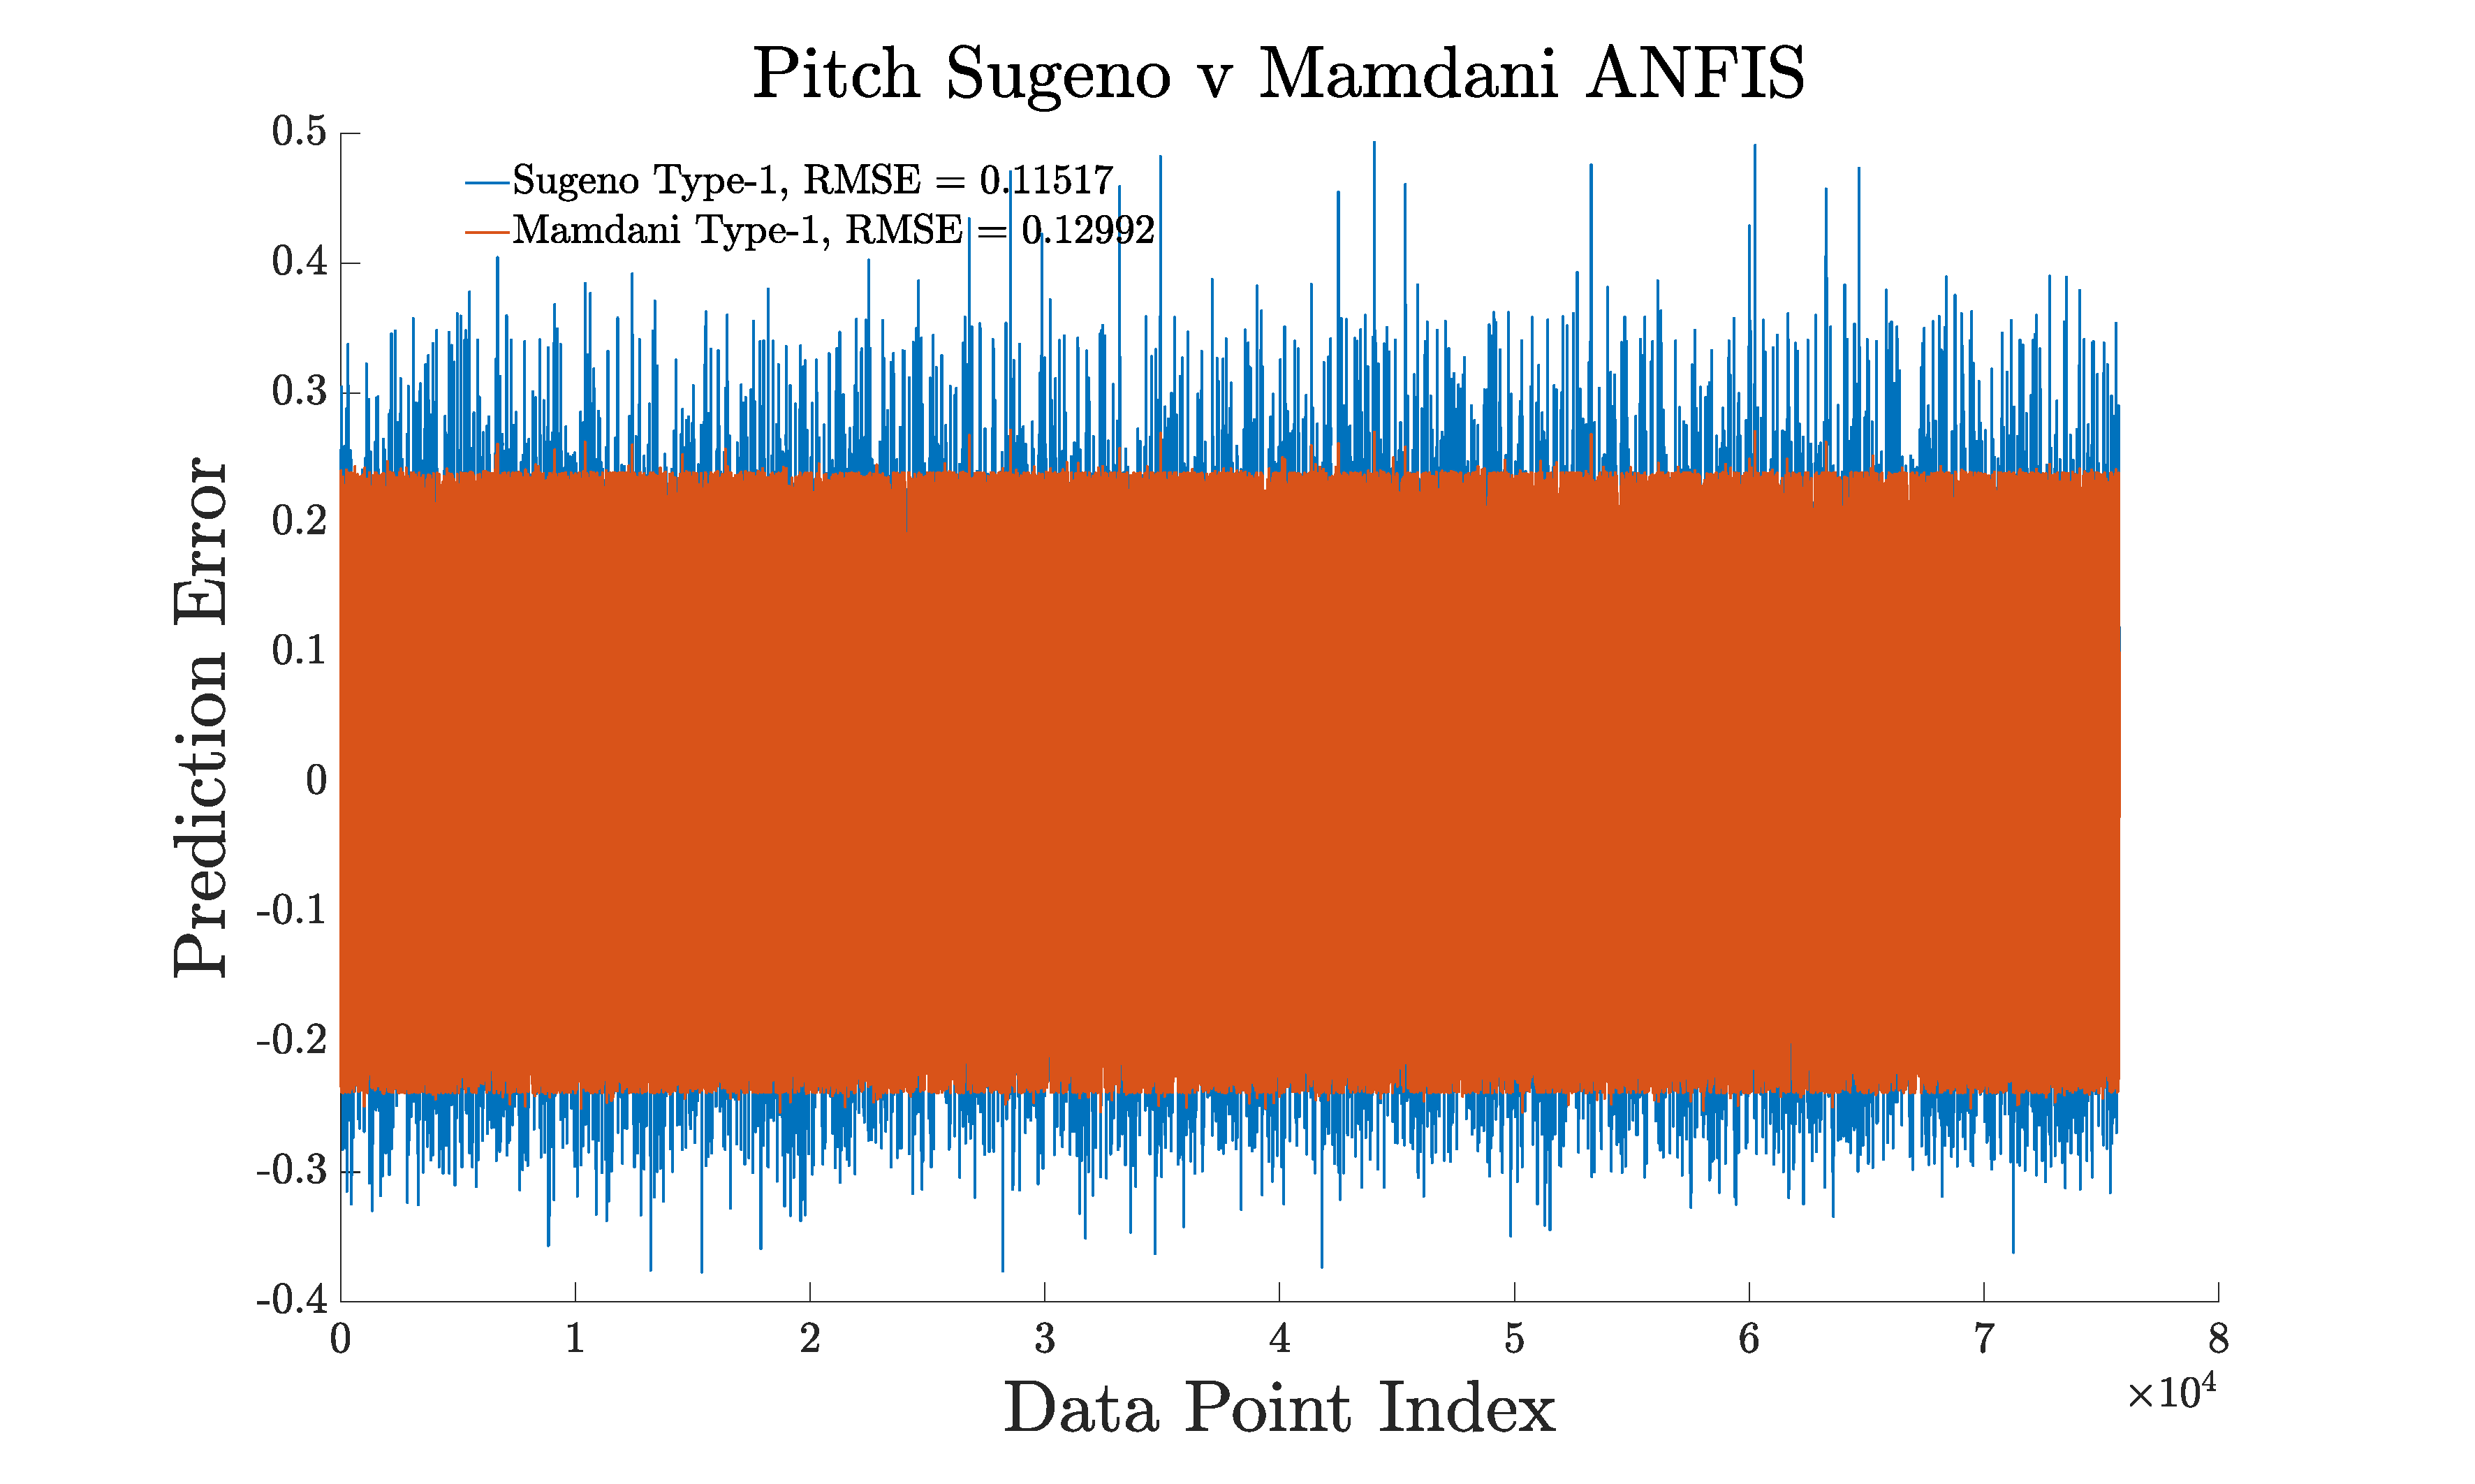
\includegraphics[height=5cm,keepaspectratio]{img/Pitch SvM.pdf}
        \caption{RMSE results for the best Sugeno and Mamdani Configurations for Pitch Output}
        \label{fig:pitch_SvM}
    \end{minipage}
\end{figure}
\begin{figure}[H]
    \centering
    \begin{minipage}[b]{0.45\textwidth}
        \centering
        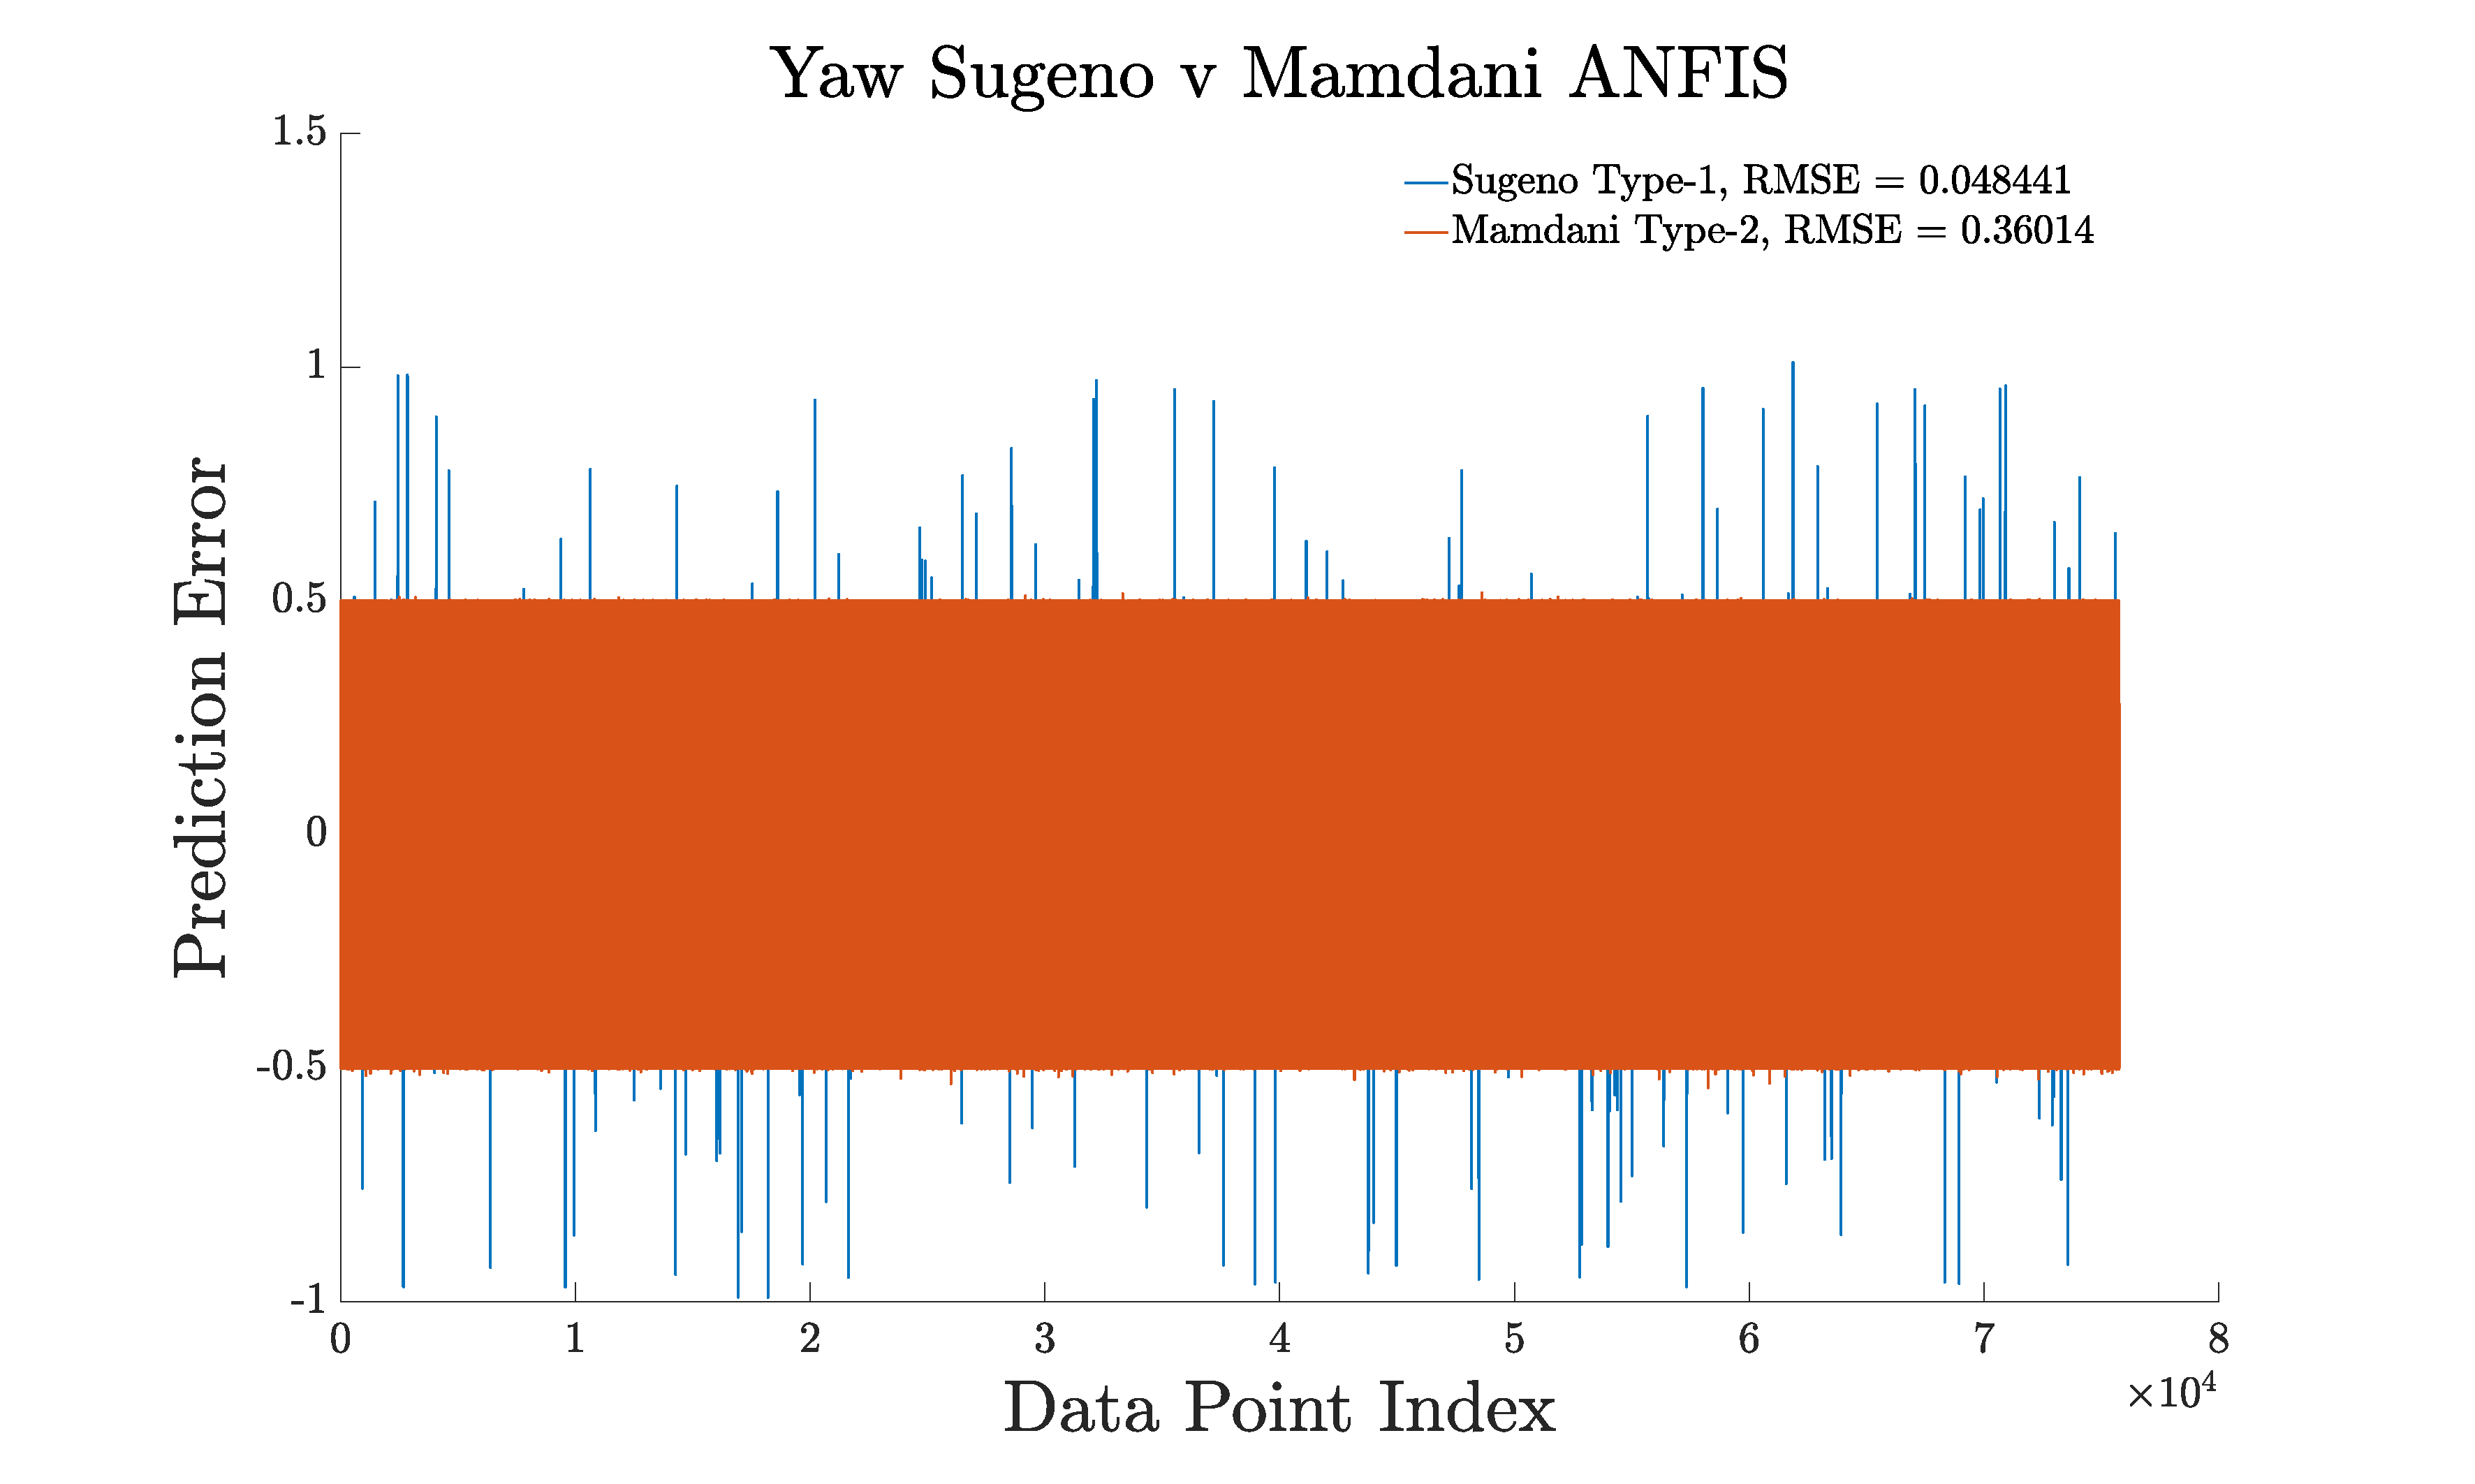
\includegraphics[height=5cm,keepaspectratio]{img/Yaw SvM.pdf}
        \caption{RMSE results for the best Sugeno and Mamdani Configurations for Yaw Output}
        \label{fig:yaw_SvM}
    \end{minipage}
    \hfill
    \begin{minipage}[b]{0.45\textwidth}
        \centering
        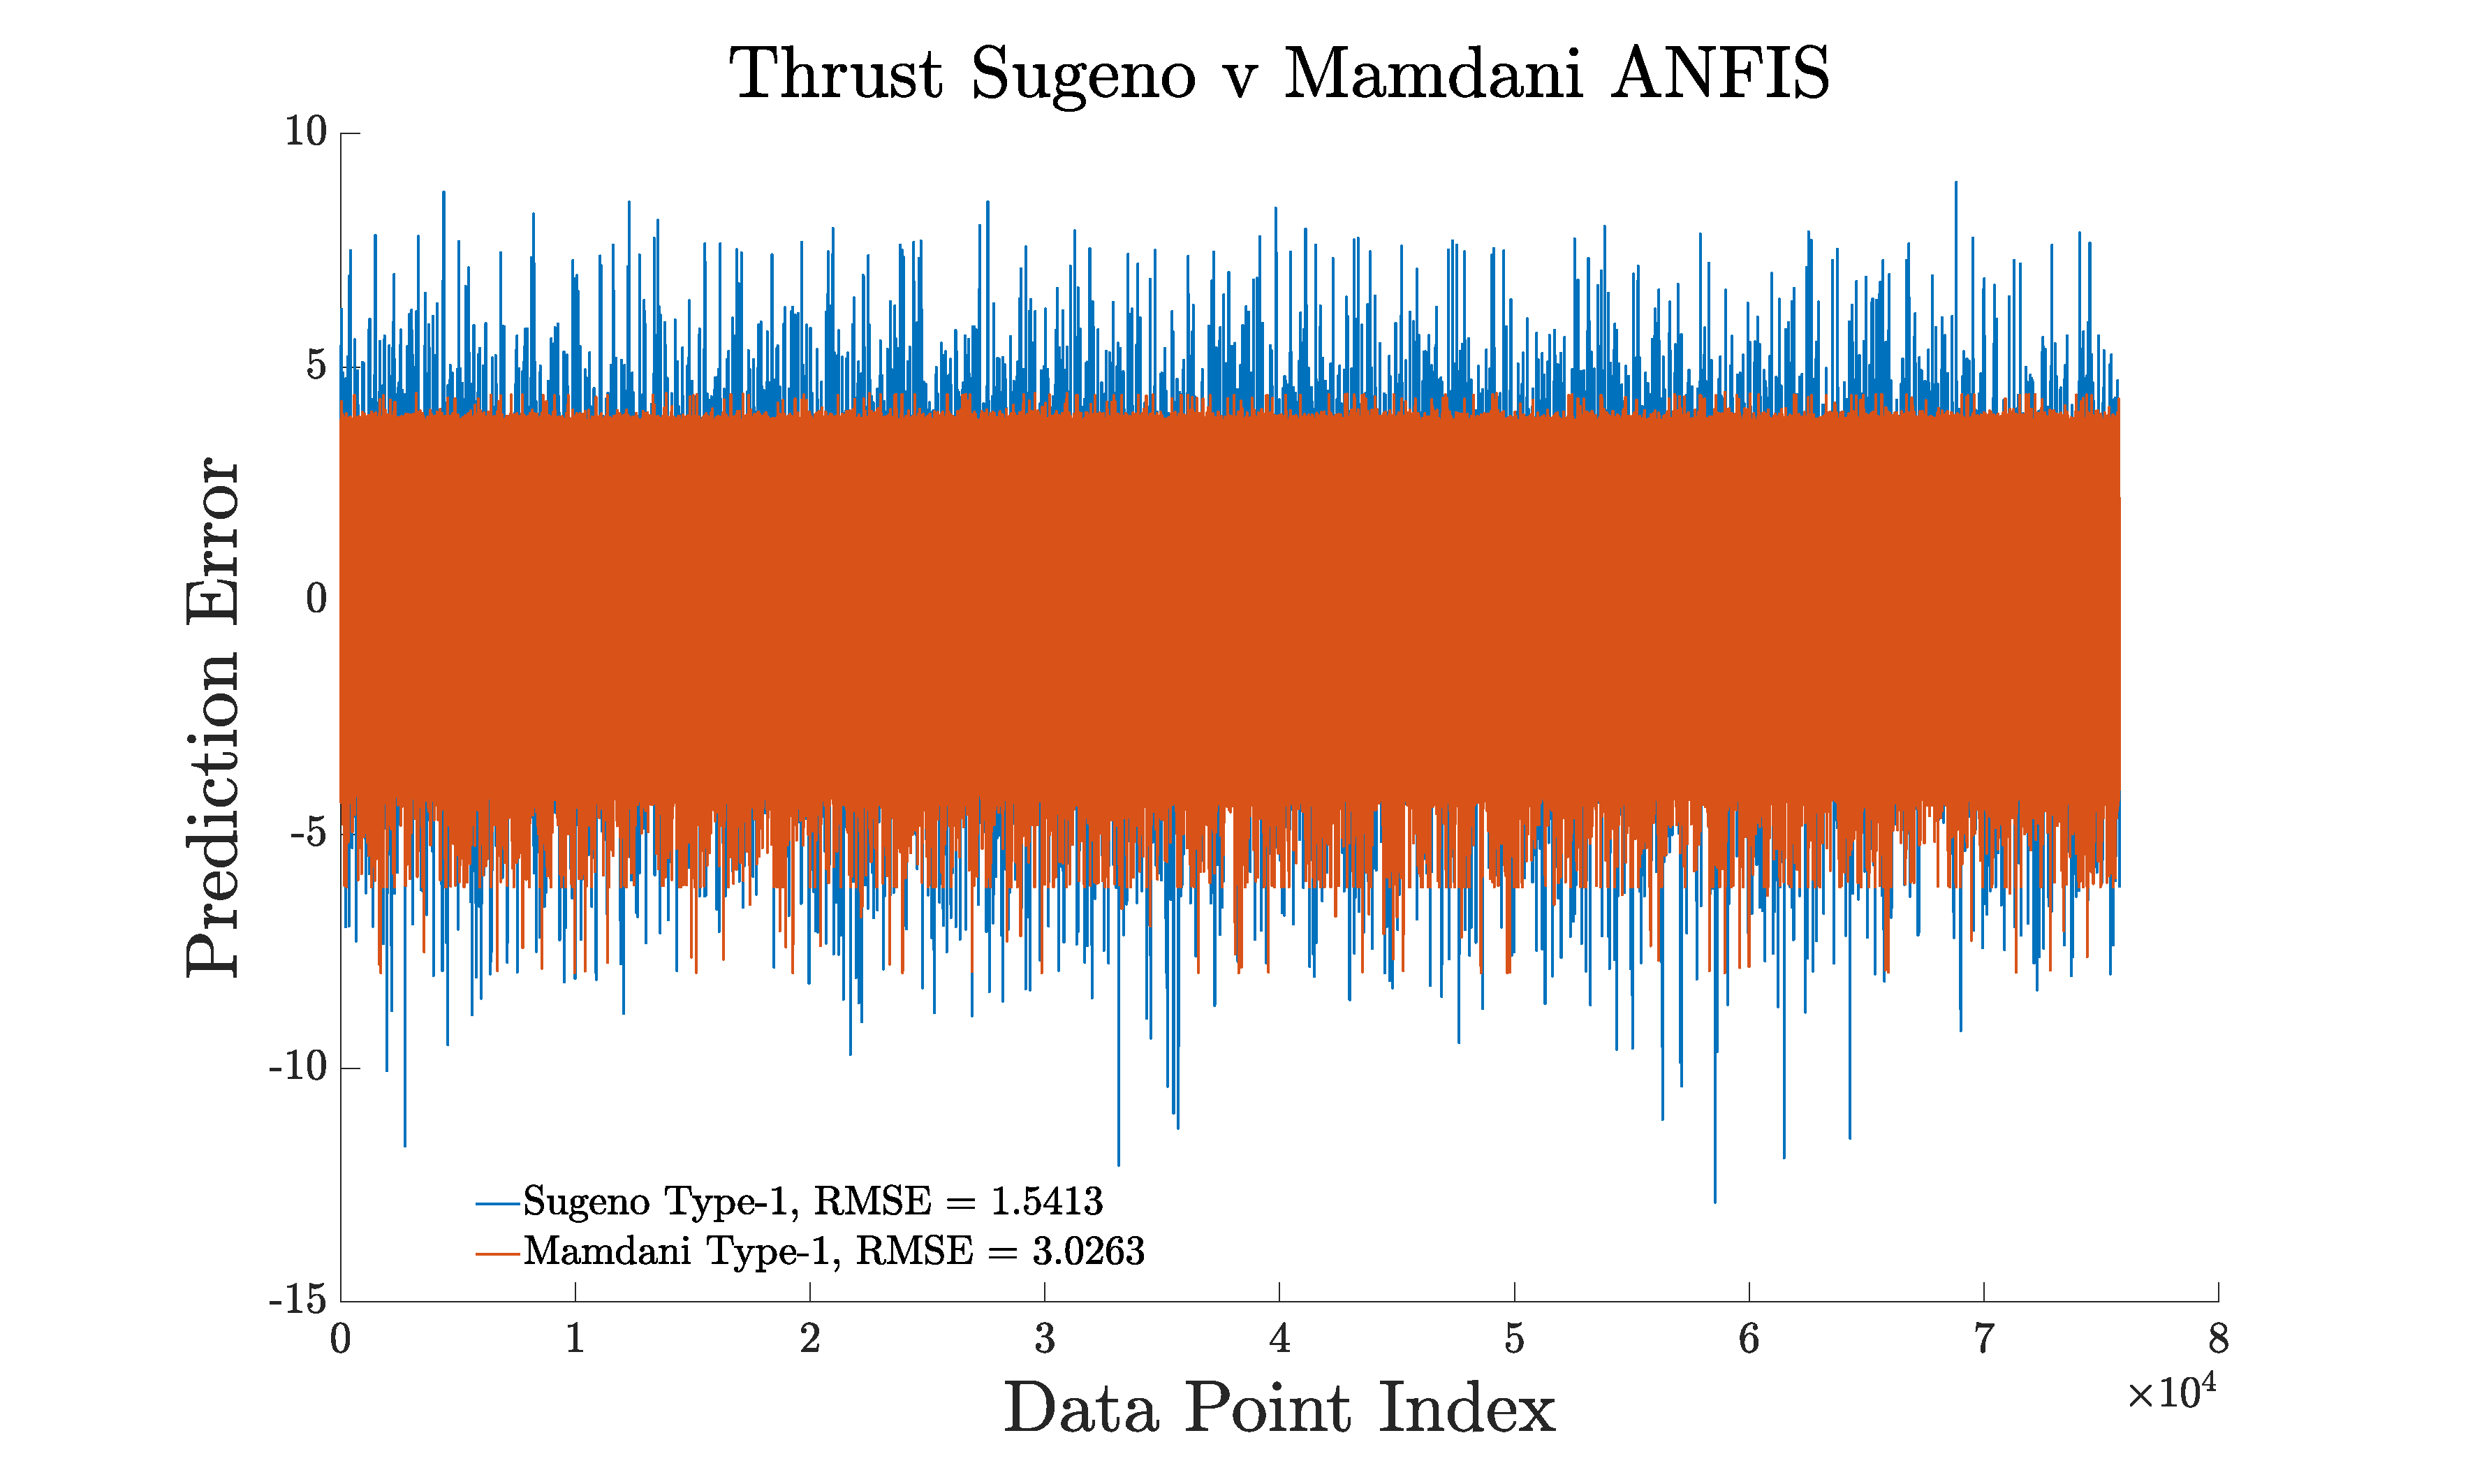
\includegraphics[height=5cm,keepaspectratio]{img/Thrust SvM.pdf}
        \caption{RMSE results for the best Sugeno and Mamdani Configurations for Thrust Output}
        \label{fig:thrust_SvM}
    \end{minipage}
\end{figure}
It was difficult to understand the performance of the models from RMSE as these are judged relative to the range of the output, therefore, the normalised RMSE was calculated. 
\begin{equation}
\text{Normalised RMSE} = \frac{\text{RMSE}}{\text{Range}}
\end{equation}
The Normalised Root Mean Square Error results of the ANFIS for each output is shown in Table \ref{tab:table_errors}. A good Normalised Root Mean Square Error (NRMSE) is highly dependent on the application. For UAV imaging, a NRMSE of 15\% or less is generally found \cite{zain4}. Table \ref{tab:table_errors} indicates that the prediction of Roll and Yaw are under this threshold at 13.2\% and 4.8\% respectively and therefore are accurate predictions. However, the thrust and especially pitch may not be as accurate as desired at 19.1\% and 24.1\% respectively. For this application, we would argue a 19.2\% NRMSE for thrust is unlikely to pose significant problems and the fact that it does not meet the 15\% found in literature is not problematic as we believe imaging prediction requires higher precision. However the 24.1\% NRMSE for Pitch could provide complications as this error is significantly higher than the 15\% seen in literature.
\begin{table}[H]
\centering
    \begin{tabular}{@{}lllll@{}}
        \toprule
        & Roll   & Pitch   & Yaw      & Thrust \\
        \midrule
        RMSE of   optimal configuration & 0.0631 & 0.11517 & 0.048441 & 1.5413 \\
        Normalised RMSE of optimal configuration & 0.1320 & 0.2411  & 0.04844  & 0.1909 \\
        \bottomrule     
    \end{tabular}
    \caption{RMSE and Normalised RMSE Errors for each output's best ANFIS Configuration}
    \label{tab:table_errors}
\end{table}
\section{Control Response Results}
Using the best ANFIS configurations found in Section 5.1, these design decisions were implemented into the simulator as shown in Figure \ref{fig:Hybrid Control}. Consequently, the simulator was tested using the PID controller and the Fuzzy Logic Controller and the error in position and computational power were compared. The scenarios are outlined in Chapter 3. (Figures \ref{fig:3_3_scenario1}, \ref{fig:3_3_scenario2}, \ref{fig:3_3_scenario3}, \ref{fig:3_3_scenario4} and \ref{fig:3_3_scenario5})

In order to evaluate the error in control response and accuracy of the controllers, the percentage error in position was calculated for each scenario as shown below. 
\begin{align}
\textrm{{Error in Position}}_{x} &= \frac{{\textrm{{Desired Position in }} x - \textrm{{Actual Position in }} x}}{{\textrm{{Desired Position in }} x}} \\
\textrm{{Error in Position}}_{y} &= \frac{{\textrm{{Desired Position in }} y - \textrm{{Actual Position in }} y}}{{\textrm{{Desired Position in }} y}} \\
\textrm{{Error in Position}}_{z} &= \frac{{\textrm{{Desired Position in }} z - \textrm{{Actual Position in }} z}}{{\textrm{{Desired Position in }} z}}\label{eq:zain1}
\end{align}

These errors in position were plotted against time to represent the control response. As the time interval was relatively small, at \SI{0.01}{\second}, the percentage error in position signal was relatively noisy therefore a moving average filter was applied. Using classical moving average filter methods \cite{zain2}, a span of 10 was used through such that an average is calculated for every second. This smoothed the control response curves and helped interpret the results. We used literature on unmanned aerial navigation to help set thresholds of error in position to analyse against. The results of a research paper by Ashraf \textit{et al} showed that their minimum average percentage error (in this case deviated from path length) was 2.19\% \cite{zain8}. After plotting our results and using this information, two threshold of 2\% and 10\% were set to analyse our plots against. The 10\% threshold was set as we thought it provided interesting insights into the speed of the two controllers towards the beginning of our simulations. 

\subsection{Scenario 1}

Scenario 1 (shown in Figure \ref{fig:3_3_scenario1}) was the most basic scenario with no obstacles, and two way-points to test the movement of the drone using each controller in open air. The control response for the error in position $x$, $y$ and $z$ against time can be seen in Figures \ref{fig:Response1x}, \ref{fig:Response1y} and \ref{fig:Response1z}. From Figures \ref{fig:Response1x} and \ref{fig:Response1y} we can see, in both cases, the PID controller has a faster response to 10\% error in position. However, for the response of error in position $x$, both the ANFIS and PID controllers reach 2\% error in position at the same time and the ANFIS controller gets to below 2\% whilst the PID maintains this error throughout the simulation. In the case of the error in position $y$, despite having a slower response to 10\% error, the ANFIS controller has a faster response to 2\% error. Both of these responses indicate that the PID controller is quicker than the ANFIS controller at the start of the simulation and then is quicker during the middle of the simulation resulting in the overall response for the ANFIS controller being better for the error in position $x$ and $y$. 

Figure \ref{fig:Response1z} shows that the ANFIS controller has large spikes in error in position $z$, compared with the PID controller which does not. This indicates anomalous control response signals due to training errors. However, despite these spikes, the drone reaches the destination in Scenario 1 quicker using the ANFIS controller compared with the PID controller. (ANFIS controller took \SI{16.18}{\second} whereas the PID controller took \SI{20.97}{\second}).
\begin{figure}[H]
    \centering
    \begin{minipage}[b]{0.45\textwidth}
        \centering
        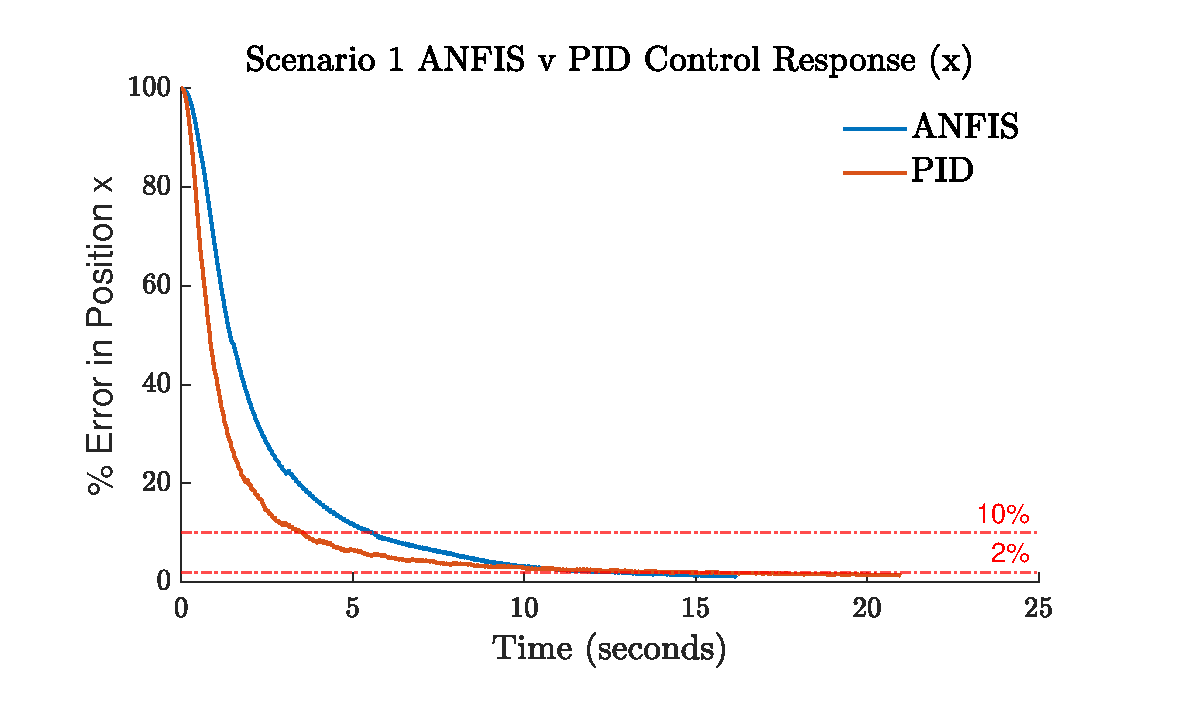
\includegraphics[height=5cm,keepaspectratio]{img/Scenario 1 Error in x Position.pdf}
        \caption{Scenario 1 Control Response (Error between Desired position $x$ and Actual position $x$) for PID and ANFIS Control}
        \label{fig:Response1x}
    \end{minipage}
    \hfill
    \begin{minipage}[b]{0.45\textwidth}
        \centering
        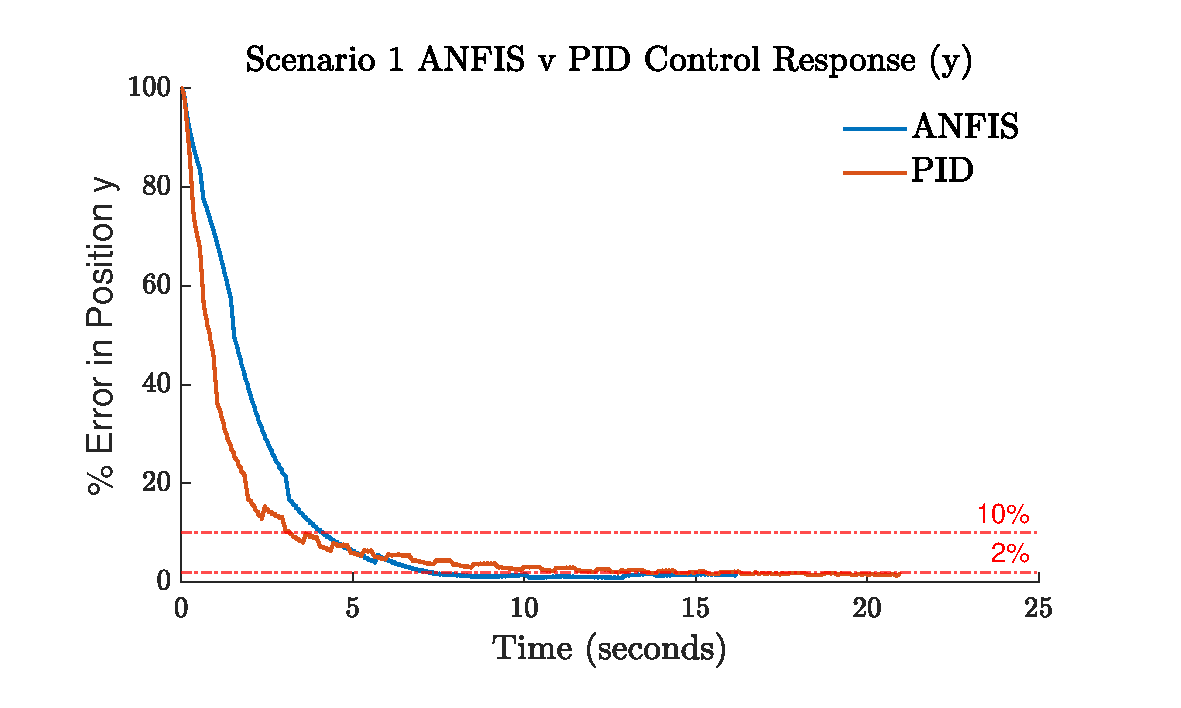
\includegraphics[height=5cm,keepaspectratio]{img/Scenario 1 Error in y Position.pdf}
        \caption{Scenario 1 Control Response (Error between Desired position $y$ and Actual position $y$) for PID and ANFIS Control}
        \label{fig:Response1y}
    \end{minipage}
\end{figure}
\begin{figure}[H]
    \centering
    \begin{minipage}[b]{0.45\textwidth}
        % empty minipage
    \end{minipage}
    \hfill
    \begin{minipage}[b]{0.45\textwidth}
        \centering
        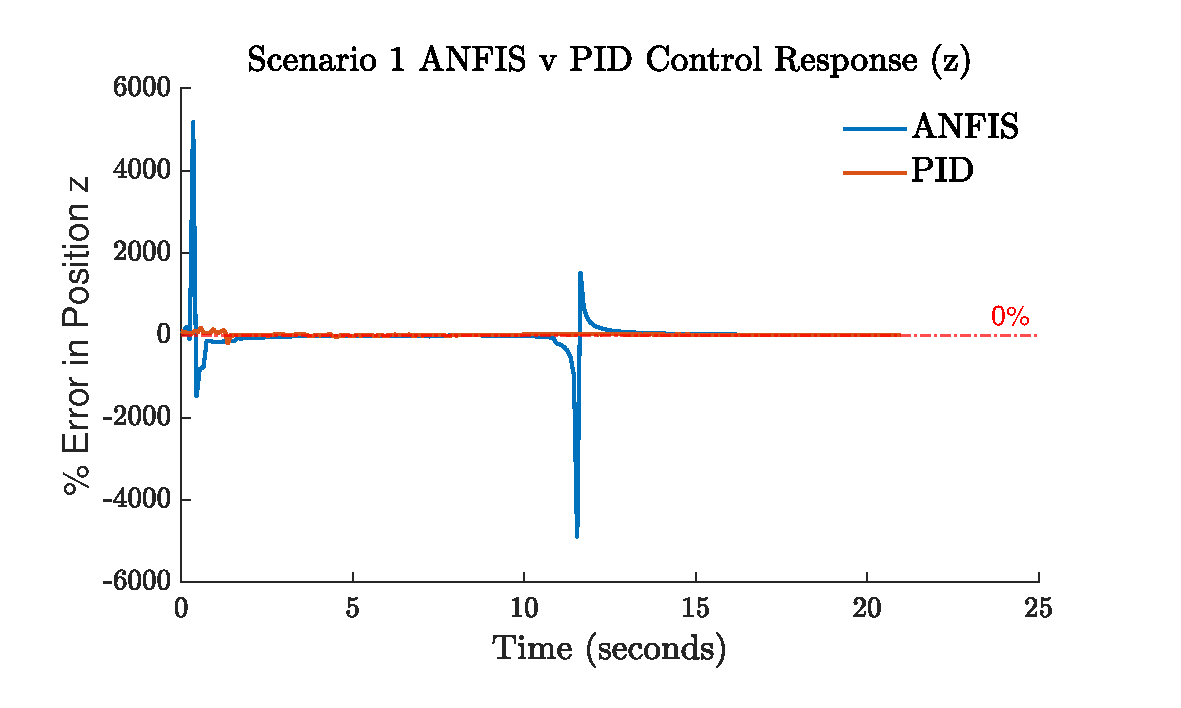
\includegraphics[height=5cm,keepaspectratio]{img/Scenario 1 Error in z Position.pdf}
        \caption{Scenario 1 Control Response (Error between Desired position $z$ and Actual position $z$) for PID and ANFIS Control}
        \label{fig:Response1z}
    \end{minipage}
    \hfill
    \begin{minipage}[b]{0.45\textwidth}
        % empty minipage
    \end{minipage}
\end{figure}

\subsection{Scenario 2}

Scenario 2 (shown in Figure \ref{fig:3_3_scenario2}) was another basic scenario with only two obstacles, both short in height and width, and one of which obstructed the path of the drone. The control response for the error in position $x$, $y$ and $z$ against time can be seen in Figures \ref{fig:Response2x}, \ref{fig:Response2y} and \ref{fig:Response2z}. Figures \ref{fig:Response2x} and \ref{fig:Response2y} shows that the PID controller has a faster response than the ANFIS controller to the 10\% error threshold in both the error in position $x$ and $y$. However, the ANFIS controller's response is quicker below this 10\% threshold meaning the ANFIS controller reaches the 2\% threshold faster than the PID controller in both cases. 

Similar to Scenario 1, Figure \ref{fig:Response2z} shows the ANFIS controller has a spike in $z$ position which similarly is likely to be caused by a training error causing an anomalous response. As the pitch output had the largest normalised RMSE (see Table \ref{tab:table_errors}), an error in this FIS is likely to have caused this anamolous response. However, despite this, the ANFIS controller again reaches its destination 29.2\% quicker due to its faster response in positions $x$ and $y$. 

\begin{figure}[H]
    \centering
    \begin{minipage}[b]{0.45\textwidth}
        \centering
        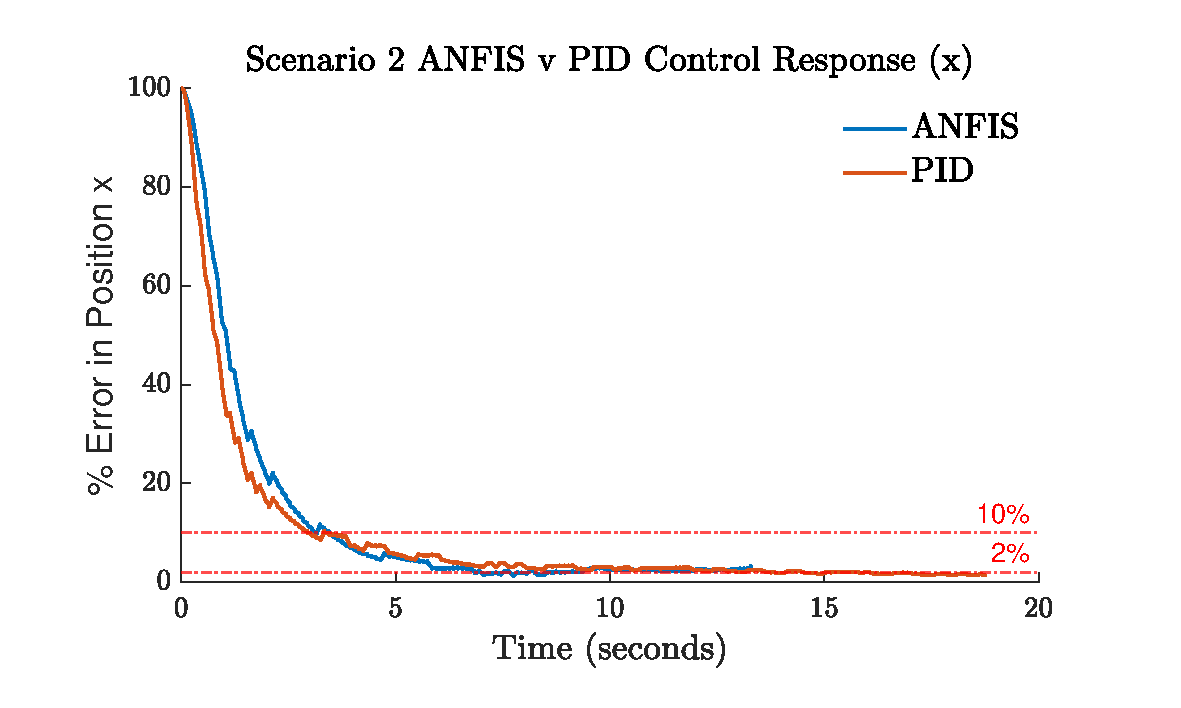
\includegraphics[height=5cm,keepaspectratio]{img/Scenario 2 Error in x Position.pdf}
        \caption{Scenario 2 Control Response (Error between Desired position $x$ and Actual position $x$) for PID and ANFIS Control}
        \label{fig:Response2x}
    \end{minipage}
    \hfill
    \begin{minipage}[b]{0.45\textwidth}
        \centering
        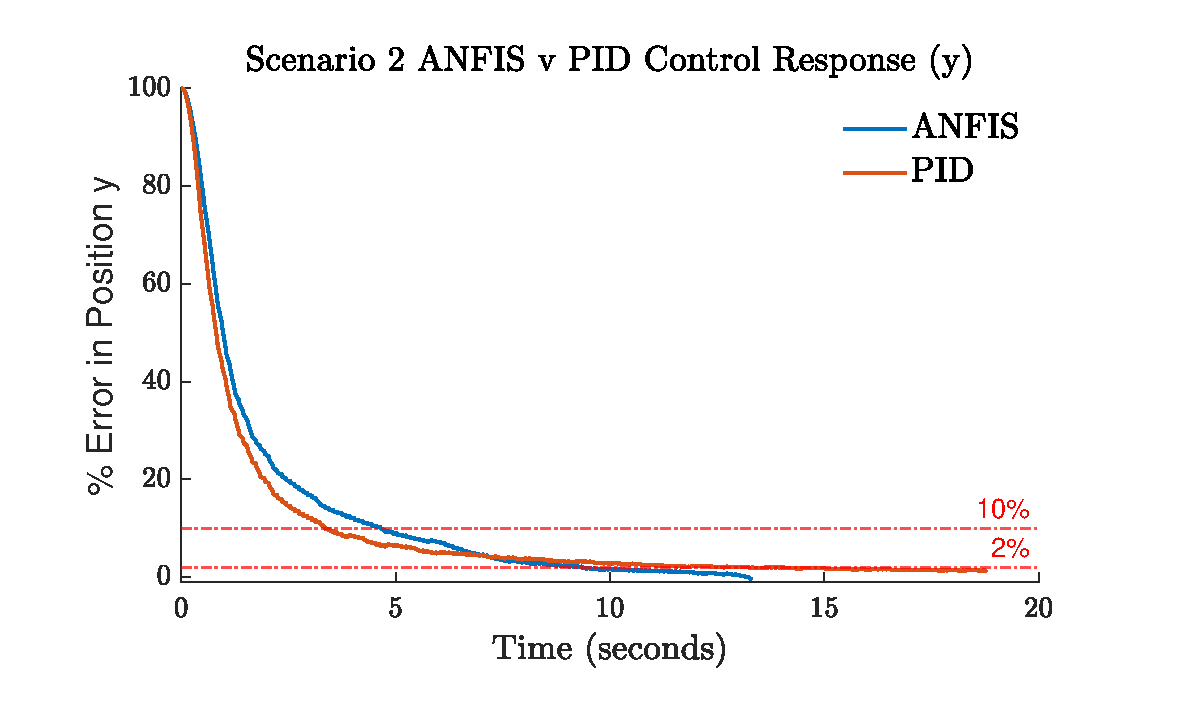
\includegraphics[height=5cm,keepaspectratio]{img/Scenario 2 Error in y Position.pdf}
        \caption{Scenario 2 Control Response (Error between Desired position $y$ and Actual position $y$) for PID and ANFIS Control}
        \label{fig:Response2y}
    \end{minipage}
\end{figure}

\begin{figure}[H]
    \centering
    \begin{minipage}[b]{0.45\textwidth}
        % empty minipage
    \end{minipage}
    \hfill
    \begin{minipage}[b]{0.45\textwidth}
        \centering
        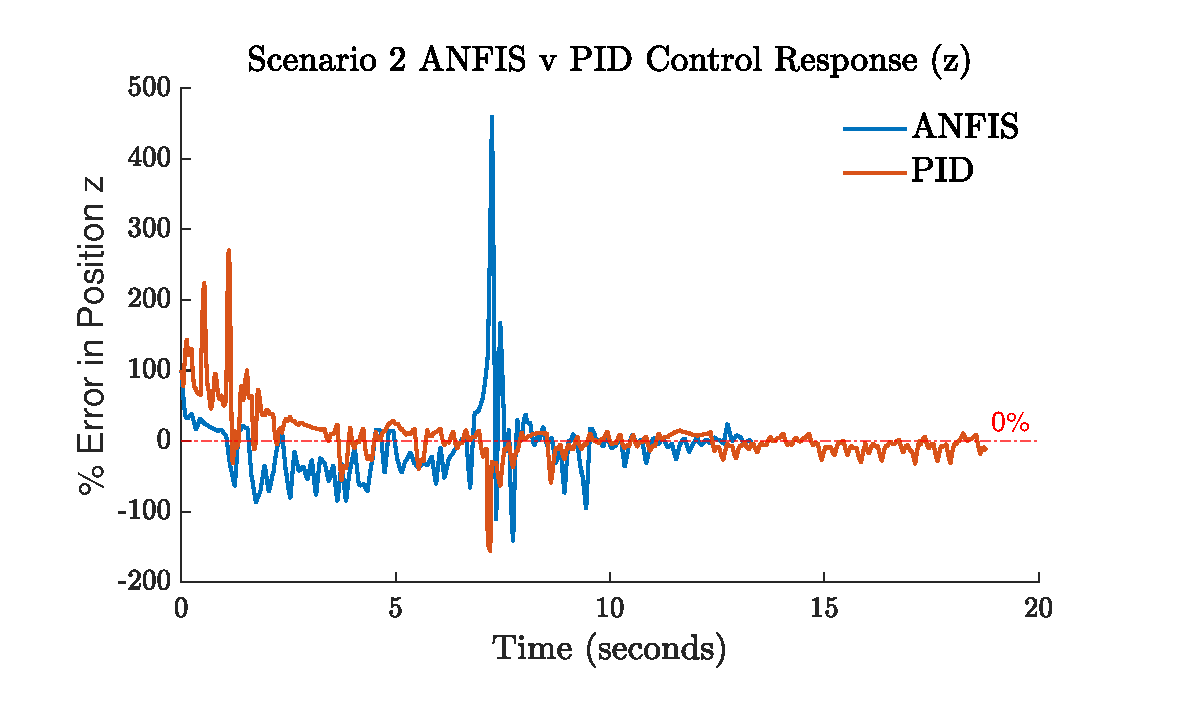
\includegraphics[height=5cm,keepaspectratio]{img/Scenario 2 Error in z Position.pdf}
        \caption{Scenario 2 Control Response (Error between Desired position $z$ and Actual position $z$) for PID and ANFIS Control}
        \label{fig:Response2z}
    \end{minipage}
    \hfill
    \begin{minipage}[b]{0.45\textwidth}
        % empty minipage
    \end{minipage}
\end{figure}

\subsection{Scenario 3}

Scenario 3 (shown in Figure \ref{fig:3_3_scenario3}) was a more challenging scenario than 1 and 2 as it tested the drones ability to go over an obstacle and therefore its ability to ascend and descend. The control response for the error in position $x$, $y$ and $z$ against time can be seen in Figures \ref{fig:Response3x}, \ref{fig:Response3y} and \ref{fig:Response3z}. Figures \ref{fig:Response3x} and \ref{fig:Response3y} shows, similar to Scenario 1 and 2, that the response of the PID controller to 10\% error in position was quicker. In this case, the PID and ANFIS response for error in position $x$ and $y$ both reach the 2\% threshold at a similar rate. 

Analogous to Scenario 1 and 2, there is a small spike in error in $z$ position, seen in \ref{fig:Response3z}, to 130\% for the ANFIS controller at the start of the simulation. Despite this spike, the ANFIS controller reaches the 10\% threshold quicker than the PID controller. However, the ANFIS controller is then slower than the PID controller to reach the 2\% threshold. The spike in error in $z$ position, as well as the slower response results in the ANFIS controller taking a longer time to reach its destination for Scenario 3. This is logically coherent with the fact that Scenario 3 was based on the drones ascending and descending movement, i.e. its $z$ position. 

\begin{figure}[H]
    \centering
    \begin{minipage}[b]{0.45\textwidth}
        \centering
        \includegraphics[height=5cm,keepaspectratio]{img/Scenario 3 Error in x Position.pdf}
        \caption{Scenario 3 Control Response (Error between Desired position $x$ and Actual position $x$) for PID and ANFIS Control}
        \label{fig:Response3x}
    \end{minipage}
    \hfill
    \begin{minipage}[b]{0.45\textwidth}
        \centering
        \includegraphics[height=5cm,keepaspectratio]{img/Scenario 3 Error in y Position.pdf}
        \caption{Scenario 3 Control Response (Error between Desired position $y$ and Actual position $y$) for PID and ANFIS Control}
        \label{fig:Response3y}
    \end{minipage}
\end{figure}

\begin{figure}[H]
    \centering
    \begin{minipage}[b]{0.45\textwidth}
        % empty minipage
    \end{minipage}
    \hfill
    \begin{minipage}[b]{0.45\textwidth}
        \centering
        \includegraphics[height=5cm,keepaspectratio]{img/Scenario 3 Error in z Position.pdf}
        \caption{Scenario 3 Control Response (Error between Desired position $z$ and Actual position $z$) for PID and ANFIS Control}
        \label{fig:Response3z}
    \end{minipage}
    \hfill
    \begin{minipage}[b]{0.45\textwidth}
        % empty minipage
    \end{minipage}
\end{figure}

\subsection{Scenario 4}

Scenario 4 (shown in Figure \ref{fig:3_3_scenario4}) was a more challenging version of scenario 2 with another way-point added and a change of height in the way-points. The control response for the error in position $x$, $y$ and $z$ against time can be seen in Figures \ref{fig:Response4x}, \ref{fig:Response4y} and \ref{fig:Response4z}. Figures \ref{fig:Response4x} and \ref{fig:Response4y} shows, much like the trend seen from the previous scenarios, that the response of the PID controller to 10\% error in position was quicker. In this case, the PID and ANFIS response for error in position $x$ and $y$ again both reach the 2\% threshold at a similar rate, however the ANFIS controller briefly spikes to just over 3\% later in the simulation, indicating a sub-optimal response given at this point. 

In line with Scenario 4, there is a small spike in error in $z$ position, seen in \ref{fig:Response3z}, to around 130\% for the ANFIS controller at the start of the simulation. Resembling Scenario 3, despite this spike, the ANFIS controller reaches the 10\% threshold quicker than the PID controller but is then slower than the PID controller to reach the 2\% threshold. Therefore, although the ANFIS controller had an overall better control response in Scenario 2, by adding another way point that caused the drone to have to change height (change in $z$ position) in Scenario 4, the drone with an ANFIS controller then had an overall worse response in this scenario. As a result, this scenario provides interesting insight into the ANFIS controller's weakness in its change in $z$ position.
\begin{figure}[H]
    \centering
    \begin{minipage}[b]{0.45\textwidth}
        \centering
        \includegraphics[height=5cm,keepaspectratio]{img/Scenario 4 Error in x Position.pdf}
        \caption{Scenario 4 Control Response (Error between Desired position $x$ and Actual position $x$) for PID and ANFIS Control}
        \label{fig:Response4x}
    \end{minipage}
    \hfill
    \begin{minipage}[b]{0.45\textwidth}
        \centering
        \includegraphics[height=5cm,keepaspectratio]{img/Scenario 4 Error in y Position.pdf}
        \caption{Scenario 4 Control Response (Error between Desired position $y$ and Actual position $y$) for PID and ANFIS Control}
        \label{fig:Response4y}
    \end{minipage}
\end{figure}

\begin{figure}[H]
    \centering
    \begin{minipage}[b]{0.45\textwidth}
        % empty minipage
    \end{minipage}
    \hfill
    \begin{minipage}[b]{0.45\textwidth}
        \centering
        \includegraphics[height=5cm,keepaspectratio]{img/Scenario 4 Error in z Position.pdf}
        \caption{Scenario 4 Control Response (Error between Desired position $z$ and Actual position $z$) for PID and ANFIS Control}
        \label{fig:Response4z}
    \end{minipage}
    \hfill
    \begin{minipage}[b]{0.45\textwidth}
        % empty minipage
    \end{minipage}
\end{figure}

\subsection{Scenario 5}
Scenario 5 (shown in Figure \ref{fig:3_3_scenario5}) had five obstacles, one of which obstructed the path of the drone, with two way-points both at the same height. This scenario aims to test the drone's ability to operate in compact spaces, using obstacle avoidance, but does not require any significant change in height (unless needed to avoid obstacle). Figures \ref{fig:Response5x} and \ref{fig:Response5y} align with the trend seen from the previous scenarios, that the response of the PID controller to 10\% error in position was faster. The PID and ANFIS response for error in position $y$ both reach the 2\% threshold at a similar rate however the ANFIS response reaches a lower error (ANFIS reaches minimum of 0.23\% error whereas PID reaches minimum of 0.78\% error). For the error in position $x$, the PID response for the error reaches the 2\% threshold quicker. 

Figure \ref{fig:Response5z} shows that for the error in position $z$ both responses are noisy. The PID response has multiple spikes and a highly noisy response compared with the ANFIS controller which has fewer spikes and a less noisy response, These responses are likely to be noisy as the desired position $z$ is near zero, therefore any small changes in actual $z$ will result in a very large error in position $z$ (as in \eqref{eq:zain1} desired $z$ position is the denominator). 

Despite the superior performance not clearly shown in Figures \ref{fig:Response5x} \ref{fig:Response5y} and \ref{fig:Response5z}, the drone using the ANFIS controller reaches its destination 23.8\% quicker, indicating the overall control response is better. Therefore, this supports the trend that the ANFIS controller performs better in scenarios with little change in $z$ position. 
\begin{figure}[H]
    \centering
    \begin{minipage}[b]{0.45\textwidth}
        \centering
        \includegraphics[height=5cm,keepaspectratio]{img/Scenario 5 Error in x Position.pdf}
        \caption{Scenario 5 Control Response (Error between Desired position $x$ and Actual position $x$) for PID and ANFIS Control}
        \label{fig:Response5x}
    \end{minipage}
    \hfill
    \begin{minipage}[b]{0.45\textwidth}
        \centering
        \includegraphics[height=5cm,keepaspectratio]{img/Scenario 5 Error in y Position.pdf}
        \caption{Scenario 5 Control Response (Error between Desired position $y$ and Actual position $y$) for PID and ANFIS Control}
        \label{fig:Response5y}
    \end{minipage}
\end{figure}

\begin{figure}[H]
    \centering
    \begin{minipage}[b]{0.45\textwidth}
        % empty minipage
    \end{minipage}
    \hfill
    \begin{minipage}[b]{0.45\textwidth}
        \centering
        \includegraphics[height=5cm,keepaspectratio]{img/Scenario 5 Error in z Position.pdf}
        \caption{Scenario 5 Control Response (Error between Desired position $z$ and Actual position $z$) for PID and ANFIS Control}
        \label{fig:Response5z}
    \end{minipage}
    \hfill
    \begin{minipage}[b]{0.45\textwidth}
        % empty minipage
    \end{minipage}
\end{figure}

\subsection{Computational Power Results}
Computational power was simply evaluated for each scenario using the ``profiler'' functionality in MATLAB, giving a report on the peak and allocated computational memory used for the simulations, as well as the simulation time. As this measure could vary based on the computational device used, the same laptop under the same conditions (i.e. no other applications running on the device and laptop is on charge) and the average of five simulations in each case was taken. The machine used to collect the results was the AMD Ryzen 7 5800U with Radeon Graphics laptop, with a RAM of 8.00 GB (7.35GB usable). 

The results of the allocated memory and peak memory used for each scenario for both the ANFIS and PID controller are shown in Figures \ref{fig:alloc_memory} and \ref{fig:peak_memory}. Figure \ref{fig:peak_memory} shows that the peak memory used is very similar for all scenarios, with the ANFIS having a slightly higher peak memory usage in four out of the five scenarios. This indicates the ANFIS and PID controllers have similar peak computational requirements, however the ANFIS generally has a slightly higher maximum power requirement. 

Figure \ref{fig:alloc_memory} shows that the allocated memory used is higher for the ANFIS controller in all cases apart from Scenario 2. This may be because the control response was especially faster for this scenario, with the ANFIS controlled drone reaching its destination 29.2\% quicker than the PID. However in all the other scenarios, the ANFIS has a higher allocated memory. Scenario 4 shows a particularly higher allocated memory for the ANFIS controller, likely due to the worse control response discussed earlier. 
\begin{figure}[H]
    \centering
    \includegraphics[width = 0.7\textwidth]{img/Allocated Computational Power.pdf}
    \caption{Allocated Computational Memory used by ANFIS and PID controllers for each scenario (labels show the difference in the value for ANFIS relative to the PID result)}
    \label{fig:alloc_memory}
\end{figure}
\begin{figure}[H]
    \centering
    \includegraphics[width = 0.7\textwidth]{img/Peak Computational Power.pdf}
    \caption{Peak Computational Memory used by ANFIS and PID controllers for each scenario (labels show the difference in the value for ANFIS relative to the PID result)}
    \label{fig:peak_memory}
\end{figure}

The results for computational time, i.e. the actual time taken by the machine to perform the simulation (not be confused with the ``simulation time'' which is the time the drone takes to reach its destination) were also investigated for each scenario and are plotted in Figure \ref{fig:comp_time}. The results align with the findings from the control response apart from Scenario 1. In Scenarios 3 and 4 the ANFIS controller had a considerably higher computational time (46.8\% and 41.2\% respectively) which correlates with the slower control response in these scenarios. The ANFIS controller had a lower computational time than the PID controller in Scenarios 2 and 5, again analogous to the control response times. The ANFIS controller unusually had a slightly higher computational time in Scenario 1 which was against the trend scene in the other four scenarios. 

The computational memory results show that the ANFIS controller overall had a slightly higher computational memory usage and therefore is likely to require higher computational requirements. The rationale behind this could be due to the duality of the controller requiring increased computation. As a result of having to decide whether to use a PID or ANFIS response, the dual ANFIS controller uses more computational memory. This is supported by the computational time results correlating with the control response results and therefore the ANFIS controller having a shorter computational time for the scenarios with a relatively minimal change in height. 
\begin{figure}[H]
    \centering
    \includegraphics[width = 0.7\textwidth]{img/Computational Time.pdf}
    \caption{Computational Time taken by ANFIS and PID controllers for each scenario (labels show the difference in the value for ANFIS relative to the PID result)}
    \label{fig:comp_time}
\end{figure}
\chapter{Conclusions and Future Work} 
\section{Conclusions}
The aim of this report was to gather a substantial dataset from drone simulations, pre-process this dataset and train an ANFIS model, implement this into the drone simulator and benchmark the performance against a PID controller. Through the analysis of RMSE of test data, a tuned Sugeno Type-1 ANFIS was judged to be the best configuration for the drone control ANFIS and therefore was implemented into the simulator. Due to the inability to extrapolate, a hybrid PID-ANFIS controller was implemented into the simulator and compared against a PID controller. Overall, the Adaptive Neuro-Fuzzy Inference System (ANFIS) implementation in drone control performed better than the PID controller in scenarios where the drone has minimal change in height. 

In terms of control response, the ANFIS controller performed better than the PID controller in three out of five of the scenarios tested with a reduction in time to destination of 22.8\% in Scenario 1, 29.2\% in Scenario 2 and 23.8\% in Scenario 5. Additionally, for Scenarios 2 and 5, the computational power needed for the controller was reduced by 24.9\% in Scenario 2 and 18.9\% in Scenario 5. This decline in computational time to destination is due to the effective training and tuning of the ANFIS, meaning that the controller does not have to use calculations to determine its control response and can instead effectively and quickly use its trained fuzzy inference system to determine the control response to be sent to the quadrotor. However, the ANFIS controller performed worse than the PID controller in terms of both control response and computational time in Scenarios 3 and 4. Through the nature of these scenarios, both requiring significant relative changes in height as well as the interpretation from the control response for the error in position $z$, it is possible to conclude that the ANFIS' limitation is in scenarios where the height changes significantly. The most plausible explanation for this is the relatively high NRMSE for the pitch output at 24.1\% meaning the ANFIS produced sub-optimal responses resulting in the drone not effectively reducing its error in $z$ position. 

The computational memory results showed that the ANFIS controller required a slightly higher allocated memory usage, at an average of 5.98\% higher across all five scenarios, as well as a higher peak memory usage, at an average of 1.7\% higher across all five scenarios. This can be explained by the duality of the ANFIS controller resulting in the controller having to determine whether to use a PID or ANFIS control response and therefore requiring more computational memory. This weakness stems from the ANFIS' inability to extrapolate results due its defined membership functions. The ways to solve this could be to use a wider dataset or to use a more computationally efficient way to construct the dual ANFIS controller. 
\section{Future Work} 
Future work could look into building a more realistic and practical simulator from which data can be collected. Due to time-frame constraints, more advanced simulation softwares and simulators were not able to be built. Therefore, choosing to build the simulator in MATLAB may have been a limitation to the practicality and reliability of the dataset. In addition, future work could use a more extensive dataset to train the ANFIS controller. This would require powerful computers (e.g. a supercomputer cluster) in order to train the ANFIS with larger datasets of above \SI{1e6}{} datapoints. A more extensive dataset and reliable simulator would likely reduce the Normalised Root Mean Square Error found for the output variables and therefore improve the accuracy of the ANFIS response. Additionally, it would increase the range of parameters that the ANFIS controller would be trained on therefore be able to use the ANFIS response for more scenarios. 

Future work could also involve looking to optimise the construction of a dual ANFIS controller. As alluded to in the conclusion, this was the key factor that restricted the performance of the ANFIS Controller in this application. Hence, working to establish a more computational efficient way to utilise both control methods would potentially allow the ANFIS controller to outperform current methods. By reducing the computation required within the dual controller, the performance can be further improved. The Model Predictive Control (MPC) framework discussed in the literature review could be applied to the ANFIS in order to potentially reduce the computation. 

Finally, as this study used the MATLAB Fuzzy Logic Designer app released in the 2023a version, there are likely to be improvements to this application within MATLAB, or within other software. Utilising an advancement, such as being able to tune an ANFIS which has more than one output, would mean that the ANFIS controller would not need to be made up of four separate inference systems but rather could be integrated within a single fuzzy-inference system. This, in turn, could reduce the computational power required and provide a faster response. 

\newpage
\bibliographystyle{unsrtnat}
\bibliography{Refs.bib}
\newpage
\appendix
\chapter{Plots}
\begin{figure}[H]
    \centering
    \includegraphics[width = 0.8\textwidth]{img/Roll Type.pdf}
    \caption{RMSE results for Type-1 and Type-2 Configurations for Roll Output}
    \label{fig:roll_type}
\end{figure}
\begin{figure}[H]
    \centering
    \includegraphics[width = 0.8\textwidth]{img/Pitch Type.pdf}
    \caption{RMSE results for Type-1 and Type-2 Configurations for Pitch Output}
    \label{fig:pitch_type}
\end{figure}
\begin{figure}[H]
    \centering
    \includegraphics[width = 0.6\textwidth]{img/Yaw Type2.pdf}
    \caption{RMSE results for Type-1 and Type-2 Configurations for Yaw Output}
    \label{fig:yaw_type}
\end{figure}
\begin{figure}[H]
    \centering
    \includegraphics[width = 0.6\textwidth]{img/Thrust Type.pdf}
    \caption{RMSE results for Type-1 and Type-2 Configurations for Thrust Output}
    \label{fig:thrust_type}
\end{figure}
\begin{figure}[H]
    \centering
    \begin{minipage}[b]{0.45\textwidth}
        \includegraphics[height=5cm,keepaspectratio]{img/scenario1_pid_paths.eps}
        \caption{Scenario 1 Path taken using PID Drone Control}
        \label{fig:Paths1_pid}
    \end{minipage}
    \hfill
    \begin{minipage}[b]{0.45\textwidth}
        \includegraphics[height=5cm,keepaspectratio]{img/scenario1_fis_paths.eps}
        \caption{Scenario 1 Path taken using ANFIS Drone Control}
        \label{fig:Paths1_fis}
    \end{minipage}
\end{figure}
\begin{figure}[H]
    \centering
    \begin{minipage}[b]{0.45\textwidth}
        \includegraphics[height=5cm,keepaspectratio]{img/scenario2_pid_paths.eps}
        \caption{Scenario 2 Path taken using PID Drone Control}
        \label{fig:Paths2_pid}
    \end{minipage}
    \hfill
    \begin{minipage}[b]{0.45\textwidth}
        \includegraphics[height=5cm,keepaspectratio]{img/scenario2_fis_paths.eps}
        \caption{Scenario 2 Path taken using ANFIS Drone Control}
        \label{fig:Paths2_fis}
    \end{minipage}
\end{figure}
\begin{figure}[H]
    \centering
    \begin{minipage}[b]{0.45\textwidth}
        \includegraphics[height=5cm,keepaspectratio]{img/scenario3_pid_paths.eps}
        \caption{Scenario 3 Path taken using PID Drone Control}
        \label{fig:Paths3_pid}
    \end{minipage}
    \hfill
    \begin{minipage}[b]{0.45\textwidth}
        \includegraphics[height=5cm,keepaspectratio]{img/scenario3_fis_paths.eps}
        \caption{Scenario 3 Path taken using ANFIS Drone Control}
        \label{fig:Paths3_fis}
    \end{minipage}
\end{figure}
\begin{figure}[H]
    \centering
    \begin{minipage}[b]{0.45\textwidth}
        \includegraphics[height=5cm,keepaspectratio]{img/scenario4_pid_paths.eps}
        \caption{Scenario 4 Path taken using PID Drone Control}
        \label{fig:Paths4_pid}
    \end{minipage}
    \hfill
    \begin{minipage}[b]{0.45\textwidth}
        \includegraphics[height=5cm,keepaspectratio]{img/scenario4_fis_paths.eps}
        \caption{Scenario 4 Path taken using ANFIS Drone Control}
        \label{fig:Paths4_fis}
    \end{minipage}
\end{figure}
\begin{figure}[H]
    \centering
    \begin{minipage}[b]{0.45\textwidth}
        \includegraphics[height=5cm,keepaspectratio]{img/scenario5_pid_paths.eps}
        \caption{Scenario 5 Path taken using PID Drone Control}
        \label{fig:Paths5_pid}
    \end{minipage}
    \hfill
    \begin{minipage}[b]{0.45\textwidth}
        \includegraphics[height=5cm,keepaspectratio]{img/scenario5_fis_paths.eps}
        \caption{Scenario 5 Path taken using ANFIS Drone Control}
        \label{fig:Paths5_fis}
    \end{minipage}
\end{figure}
\end{document}